%% abtex2-modelo-trabalho-academico.tex, v-1.9.7 laurocesar
%% Copyright 2012-2018 by abnTeX2 group at http://www.abntex.net.br/ 
%%
%% This work may be distributed and/or modified under the
%% conditions of the LaTeX Project Public License, either version 1.3
%% of this license or (at your option) any later version.
%% The latest version of this license is in
%%   http://www.latex-project.org/lppl.txt
%% and version 1.3 or later is part of all distributions of LaTeX
%% version 2005/12/01 or later.
%%
%% This work has the LPPL maintenance status `maintained'.
%% 
%% The Current Maintainer of this work is the abnTeX2 team, led
%% by Lauro César Araujo. Further information are available on 
%% http://www.abntex.net.br/
%%
%% This work consists of the files abntex2-modelo-trabalho-academico.tex,
%% abntex2-modelo-include-comandos and abntex2-modelo-references.bib
%%

% ------------------------------------------------------------------------
% ------------------------------------------------------------------------
% abnTeX2: Modelo de Trabalho Academico (tese de doutorado, dissertacao de
% mestrado e trabalhos monograficos em geral) em conformidade com 
% ABNT NBR 14724:2011: Informacao e documentacao - Trabalhos academicos -
% Apresentacao
% ------------------------------------------------------------------------
% ------------------------------------------------------------------------

\documentclass[
	% -- opções da classe memoir --
	12pt,				% tamanho da fonte
	openany,			% capítulos começam em pág ímpar (insere página vazia caso preciso)
	oneside,			% para impressão em recto e verso. Oposto a oneside
	a4paper,			% tamanho do papel. 
	% -- opções da classe abntex2 --
	%chapter=TITLE,		% títulos de capítulos convertidos em letras maiúsculas
	%section=TITLE,		% títulos de seções convertidos em letras maiúsculas
	%subsection=TITLE,	% títulos de subseções convertidos em letras maiúsculas
	%subsubsection=TITLE,% títulos de subsubseções convertidos em letras maiúsculas
	% -- opções do pacote babel --
	english,			% idioma adicional para hifenização
	french,				% idioma adicional para hifenização
	spanish,			% idioma adicional para hifenização
	brazil				% o último idioma é o principal do documento
	]{abntex2}

\checkandfixthelayout % para garantir que o layout seja atualizado
\makeatletter
\renewcommand*{\cleardoublepage}{\clearpage}
\makeatother
% ----------------------------------------------------------
% Pacotes básicos
% ----------------------------------------------------------
\usepackage{lmodern}
\usepackage[T1]{fontenc}
\usepackage[utf8]{inputenc}
\usepackage{microtype}
\usepackage{graphicx}
\usepackage{indentfirst}
\usepackage{color}
\usepackage{emptypage}
\usepackage{float}
\usepackage{longtable}

% ----------------------------------------------------------
% Pacotes adicionais
% ----------------------------------------------------------
\usepackage{pgfplots}
\pgfplotsset{compat=1.18}

\usepackage{adjustbox}
\usepackage{ragged2e}
\usepackage{tabularx}
\usepackage{caption}
\usepackage{array}
\usepackage{chngcntr}
\usepackage{tocloft}
\usepackage{booktabs}
\usepackage{geometry}
\geometry{margin=1in}
\usepackage{lipsum}
\usepackage{placeins}
\usepackage{multirow}
\usepackage{qrcode}
\usepackage{xcolor}
\usepackage{hyperref}

% ----------------------------------------------------------
% Citações ABNT
% ----------------------------------------------------------
\usepackage[brazilian,hyperpageref]{backref}
\usepackage[alf]{abntex2cite}

\renewcommand{\backrefpagesname}{Citado na(s) página(s):~}
\renewcommand{\backref}{}
\renewcommand*{\backrefalt}[4]{
	\ifcase #1
	Nenhuma citação no texto.
	\or
	Citado na página #2.
	\else
	Citado #1 vezes nas páginas #2.
	\fi
}

% espaçamento de tabelas
\renewcommand{\arraystretch}{1.4}

% ----------------------------------------------------------
% Dados da capa e folha de rosto
% ----------------------------------------------------------
\titulo{Pousada Chalés Água de Coco}
\autor{
	\begin{tabular}{l c}
		 GUILHERME AKIO MIURA & SP3120791\\
		 GUILHERME BITTENCOURT SCHMIDT & SP313640X\\
		 KELLY RADCHELLE ARAUJO DE SOUZA & SP3123588\\
		 RAFAEL TEIXEIRA FONSECA & SP3126919\\
		 RICARDO CARRIEL DE OLIVEIRA FILHO & SP3136728
	 \end{tabular}
	 }
\local{São Paulo - SP - Brasil}
\data{2025}
\orientador{Marcelo Tavares de Santana}
%\coorientador{Equipe \abnTeX}
\instituicao{%
  IFSP - Instituto Federal de Educação, Ciência e Tecnologia de São Paulo
  \par
  Tecnologia em Análise e Desenvolvimento de Sistemas}
\tipotrabalho{Trabalho Conclusão de Curso}
% O preambulo deve conter o tipo do trabalho, o objetivo, 
% o nome da instituição e a área de concentração 
\preambulo{Projeto de Conclusão de Curso apresentado
ao Instituto Federal de Educação, Ciência e
Tecnologia de São Paulo Câmpus São Paulo,
como requisito parcial para conclusão do
curso Tecnologia em Análise e Desenvolvimento de Sistemas. 
}
% ----------------------------------------------------------
% PDF
% ----------------------------------------------------------
\definecolor{blue}{RGB}{41,5,195}

\makeatletter
\hypersetup{
	pdftitle={\@title},
	pdfauthor={\@author},
	pdfsubject={\imprimirpreambulo},
	pdfcreator={LaTeX with abnTeX2},
	colorlinks=true,
	linkcolor=blue,
	citecolor=blue,
	urlcolor=blue,
	bookmarksdepth=4
}
\makeatother

% ----------------------------------------------------------
% Float no topo de página
% ----------------------------------------------------------
\makeatletter
\setlength{\@fptop}{5pt}
\makeatother

% ----------------------------------------------------------
% QUADROS — IMPLEMENTAÇÃO CORRETA
% ----------------------------------------------------------

% nome
\newcommand{\quadroname}{Quadro}
\newcommand{\listofquadrosname}{Lista de quadros}

% cria o float "quadro"
\newfloat{quadro}{htbp}{loq}
\floatname{quadro}{\quadroname}

% lista de quadros
\newlistof{listofquadros}{loq}{\listofquadrosname}
\newlistentry{quadro}{loq}{0}

% legenda em cima (ABNT)
\captionsetup[quadro]{position=top, skip=0.5\baselineskip}

% centralizar quadros
\setfloatadjustment{quadro}{\centering}

% não reiniciar por capítulo
\counterwithout{quadro}{chapter}

% posição preferencial
\setfloatlocations{quadro}{hbtp}

%
\usepackage{float}
\floatstyle{plaintop} % faz a legenda ir para o topo
\restylefloat{quadro} %----------------------------------------------------------
% PARÁGRAFOS E ESPAÇAMENTO
% ----------------------------------------------------------
\setlength{\parindent}{1.3cm}
\setlength{\parskip}{0.2cm}

% ----------------------------------------------------------
\makeindex
% ----------------------------------------------------------

\begin{document}

% Seleciona o idioma do documento (conforme pacotes do babel)
%\selectlanguage{english}
\selectlanguage{brazil}

% Retira espaço extra obsoleto entre as frases.
\frenchspacing 

% ----------------------------------------------------------
% ELEMENTOS PRÉ-TEXTUAIS
% ----------------------------------------------------------
% \pretextual

% ---
% Capa
% ---
\imprimircapa
% ---
% ---
% Folha de rosto
% (o * indica que haverá a ficha bibliográfica)
% ---
\imprimirfolhaderosto*
% ---
% ---
% Inserir a ficha bibliografica
% ---
% Isto é um exemplo de Ficha Catalográfica, ou ``Dados internacionais de
% catalogação-na-publicação''. Você pode utilizar este modelo como referência. 
% Porém, provavelmente a biblioteca da sua universidade lhe fornecerá um PDF
% com a ficha catalográfica definitiva após a defesa do trabalho. Quando estiver
% com o documento, salve-o como PDF no diretório do seu projeto e substitua todo
% o conteúdo de implementação deste arquivo pelo comando abaixo:
%
% \begin{fichacatalografica}
%     \includepdf{fig_ficha_catalografica.pdf}
% \end{fichacatalografica}
%\begin{fichacatalografica}
%	\sffamily
%	\vspace*{\fill}					% Posição vertical
%	\begin{center}					% Minipage Centralizado
%	\fbox{\begin{minipage}[c][8cm]{13.5cm}		% Largura
%	\small
%	\imprimirautor
	%Sobrenome, Nome do autor
	
%	\hspace{0.5cm} \imprimirtitulo  / \imprimirautor. --
%	\imprimirlocal, \imprimirdata-
	
%	\hspace{0.5cm} \thelastpage p. : il. (algumas color.) ; 30 cm.\\
	
%	\hspace{0.5cm} \imprimirorientadorRotulo~\imprimirorientador\\
	
%	\hspace{0.5cm}
%	\parbox[t]{\textwidth}{\imprimirtipotrabalho~--~\imprimirinstituicao,
%	\imprimirdata.}\\
	
%	\hspace{0.5cm}
%		1. Palavra-chave1.
%		2. Palavra-chave2.
%		2. Palavra-chave3.
%		I. Orientador.
%		II. Universidade xxx.
%		III. Faculdade de xxx.
%		IV. Título 			
%	\end{minipage}}
%	\end{center}
%\end{fichacatalografica}
% ---

% ---
% Inserir errata
% ---
%\begin{errata}
%Elemento opcional da \citeonline[4.2.1.2]{NBR14724:2011}. Exemplo:

%\vspace{\onelineskip}

%FERRIGNO, C. R. A. \textbf{Tratamento de neoplasias ósseas apendiculares com
%reimplantação de enxerto ósseo autólogo autoclavado associado ao plasma
%rico em plaquetas}: estudo crítico na cirurgia de preservação de membro em
%cães. 2011. 128 f. Tese (Livre-Docência) - Faculdade de Medicina Veterinária e
%Zootecnia, Universidade de São Paulo, São Paulo, 2011.

%\begin{table}[htb]
%\center
%\footnotesize
%\begin{tabular}{|p{1.4cm}|p{1cm}|p{3cm}|p{3cm}|}
%  \hline
%   \textbf{Folha} & \textbf{Linha}  & \textbf{Onde se lê}  & \textbf{Leia-se}  \\
%    \hline
%    1 & 10 & auto-conclavo & autoconclavo\\
%   \hline
%\end{tabular}
%\end{table}

%\end{errata}
% ---

% ---
% Inserir folha de aprovação
% ---

% Isto é um exemplo de Folha de aprovação, elemento obrigatório da NBR
% 14724/2011 (seção 4.2.1.3). Você pode utilizar este modelo até a aprovação
% do trabalho. Após isso, substitua todo o conteúdo deste arquivo por uma
% imagem da página assinada pela banca com o comando abaixo:
%
% \begin{folhadeaprovacao}
% \includepdf{folhadeaprovacao_final.pdf}
% \end{folhadeaprovacao}
%
%\begin{folhadeaprovacao}

%  \begin{center}
%    {\ABNTEXchapterfont\large\imprimirautor}

%    \vspace*{\fill}\vspace*{\fill}
%    \begin{center}
%      \ABNTEXchapterfont\bfseries\Large\imprimirtitulo
%    \end{center}
%    \vspace*{\fill}
    
%    \hspace{.45\textwidth}
%    \begin{minipage}{.5\textwidth}
 %       \imprimirpreambulo
%    \end{minipage}%
%    \vspace*{\fill}
%   \end{center}
        
%   Trabalho aprovado. \imprimirlocal, 24 de novembro de 2012:

%   \assinatura{\textbf{\imprimirorientador} \\ Orientador} 
%   \assinatura{\textbf{Professor} \\ Convidado 1}
%   \assinatura{\textbf{Professor} \\ Convidado 2}
   %\assinatura{\textbf{Professor} \\ Convidado 3}
   %\assinatura{\textbf{Professor} \\ Convidado 4}
      
%   \begin{center}
%    \vspace*{0.5cm}
%    {\large\imprimirlocal}
%    \par
%    {\large\imprimirdata}
%    \vspace*{1cm}
%  \end{center}
  
%\end{folhadeaprovacao}
% ---

% ---
% Dedicatória
% ---
%\begin{dedicatoria}
%   \vspace*{\fill}
%   \centering
%   \noindent
%   \textit{ Este trabalho é dedicado às crianças adultas que,\\
%   quando pequenas, sonharam em se tornar cientistas.} \vspace*{\fill}
%\end{dedicatoria}
% ---

% ---
% Agradecimentos
% ---
%\begin{agradecimentos}
%Os agradecimentos principais são direcionados à Gerald Weber, Miguel Frasson,
%Leslie H. Watter, Bruno Parente Lima, Flávio de Vasconcellos Corrêa, Otavio Real
%Salvador, Renato Machnievscz\footnote{Os nomes dos integrantes do primeiro
%projeto abn\TeX\ foram extraídos de
%\url{http://codigolivre.org.br/projects/abntex/}} e todos aqueles que
%contribuíram para que a produção de trabalhos acadêmicos conforme
%as normas ABNT com \LaTeX\ fosse possível.

%Agradecimentos especiais são direcionados ao Centro de Pesquisa em Arquitetura
%da Informação\footnote{\url{http://www.cpai.unb.br/}} da Universidade de
%Brasília (CPAI), ao grupo de usuários
%\emph{latex-br}\footnote{\url{http://groups.google.com/group/latex-br}} e aos
%novos voluntários do grupo
%\emph{\abnTeX}\footnote{\url{http://groups.google.com/group/abntex2} e
%\url{http://www.abntex.net.br/}}~que contribuíram e que ainda
%contribuirão para a evolução do \abnTeX.

%\end{agradecimentos}
% ---

% ---
% Epígrafe
% ---
%\begin{epigrafe}
%    \vspace*{\fill}
%	\begin{flushright}
%		\textit{``Não vos amoldeis às estruturas deste mundo, \\
%		mas transformai-vos pela renovação da mente, \\
%		a fim de distinguir qual é a vontade de Deus: \\
%		o que é bom, o que Lhe é agradável, o que é perfeito.\\
%		(Bíblia Sagrada, Romanos 12, 2)}
%	\end{flushright}
%\end{epigrafe}
% ---

% ---
% RESUMOS
% ---

% resumo em português
\setlength{\absparsep}{18pt} % ajusta o espaçamento dos parágrafos do resumo
\begin{resumo}
	Este Projeto de Conclusão de Curso tem como objetivo o desenvolvimento de um sistema \textit{web} para automatizar os processos administrativos da pousada Chalés Água de Coco, que atualmente realiza a gestão de hóspedes, reservas, acomodações e controle financeiro por meio de planilhas eletrônicas no Excel. A falta de integração e a limitação desse método tornam a operação vulnerável a erros, retrabalho e dificuldade de acesso remoto às informações. Com base em uma parceria estabelecida com a pousada, foi possível realizar um levantamento detalhado dos requisitos e desenvolver uma solução personalizada, capaz de centralizar as informações em uma única plataforma, acessível via Internet. O sistema propõe melhorias significativas na organização dos dados, no controle de reservas e na geração de relatórios gerenciais, otimizando a tomada de decisões. Este projeto representa a aplicação prática dos conhecimentos adquiridos ao longo do curso, ao mesmo tempo em que oferece uma ferramenta útil para a modernização da gestão em pequenos empreendimentos do setor de hospitalidade.
	
	\textbf{Palavras-chave}: sistema \textit{web}, pousada, automação, reservas, gestão de hóspedes, controle financeiro.
\end{resumo}
% resumo em inglês
\begin{resumo}[Abstract]
	\begin{otherlanguage*}{english}
		This Final Paper aims to develop a web-based system to automate the administrative processes of the inn Chalés Água de Coco, which currently manages guests, reservations, accommodations, and financial control through Excel spreadsheets. The lack of integration and limitations of this manual method make operations prone to errors, rework, and hinder remote access to information. Based on a partnership established with the inn, it was possible to conduct a detailed requirements analysis and develop a customized solution capable of centralizing data on a single, internet-accessible platform. The system brings significant improvements in data organization, reservation management, and the generation of management reports, optimizing decision-making. This project represents the practical application of the knowledge acquired, while also delivering a useful tool to modernize management practices in small hospitality businesses.
		
		\vspace{\onelineskip}
		
		\noindent 
		\textbf{Keywords}: web system, inn, automation, reservations, guest management, financial control.
	\end{otherlanguage*}
\end{resumo}
% ---
% inserir lista de ilustrações
% ---
\pdfbookmark[0]{\listfigurename}{lof}
\listoffigures*
\cleardoublepage
% ---
% ---
% inserir lista de quadros
% ---
\pdfbookmark[0]{\listofquadrosname}{loq}
\listofquadros*
\cleardoublepage
% ---
% ---
% inserir lista de tabelas
% ---
\pdfbookmark[0]{\listtablename}{lot}
\listoftables*
\cleardoublepage
% ---
% ---
% inserir lista de abreviaturas e siglas
% ---
\begin{siglas}
  \item[ABNT] Associação Brasileira de Normas Técnicas
  \item[AWS]	Amazon Web Services
  \item[CSRF]	Cross-Site Request Forgery (Falsificação de Requisição entre Sites)
  \item[CSS]	Cascading Style Sheets
  \item[HTML]	HyperText Markup Language
  \item[HTTP]	Hypertext Transfer Protocol
  \item[HTTPS]	Hypertext Transfer Protocol Secure
  \item[IP]	Internet Protocol
  \item[LGPD]	Lei Geral de Proteção de Dados
  \item[MVC]	Model-View-Controller
   (Modelo-Visão-Controlador)
  \item[MVP] 	Minimum Viable Product (Produto Mínimo Viável)
  \item[MTV]	Model-Template-View (Modelo-Template-Visualização)
  \item[ORM]	Object-Relational Mapper (Mapeador Objeto-Relacional)
  \item[PBKDF2]	Password-Based Key Derivation Function 2
  \item[POST]	Post Method (Método de Envio via HTTP)
  \item[SQL]	Structured Query Language
  \item[SSL]	Secure Sockets Layer
  \item[TLS]	Transport Layer Security
  \item[URL]	Uniform Resource Locator
  \item[XSS]	Cross-Site Scripting (Script Entre Sites)
\end{siglas}
% ---
% ---
% inserir lista de símbolos
% ---
%\begin{simbolos}
%  \item[$ \Gamma $] Letra grega Gama
%  \item[$ \Lambda $] Lambda
%  \item[$ \zeta $] Letra grega minúscula zeta
%  \item[$ \in $] Pertence
%\end{simbolos}
% ---

% ---
% inserir o sumario
% ---
\pdfbookmark[0]{\contentsname}{toc}
\tableofcontents*
\cleardoublepage
% ---



% ----------------------------------------------------------
% ELEMENTOS TEXTUAIS
% ----------------------------------------------------------
\textual

% ----------------------------------------------------------
% Introdução (exemplo de capítulo sem numeração, mas presente no Sumário)
% --------------------------------------------------------------------------------------------------------------
\chapter{Introdução}
% ----------------------------------------------------------

A transformação digital tem impactado significativamente a forma como empresas de diversos segmentos gerenciam suas atividades operacionais e estratégicas. No setor de hospitalidade, essa mudança tem se mostrado essencial para garantir maior eficiência, organização e qualidade no atendimento ao cliente. Segundo dados do Ministério do Turismo, cerca de 89\% dos empreendimentos no setor de turismo no Brasil são compostos por micro e pequenas empresas~\cite{mtur}, evidenciando a importância de soluções tecnológicas adequadas para esse perfil de organização.

Apesar dos avanços tecnológicos, muitas pousadas e hotéis de pequeno porte ainda utilizam métodos manuais ou ferramentas limitadas, como planilhas eletrônicas, para controlar reservas, hospedagens e finanças. Essa prática, embora funcional em um primeiro momento, apresenta restrições consideráveis, como risco elevado de erros, dificuldade de atualização em tempo real e ausência de acessibilidade remota~\cite{gestaopro}.

No caso da Pousada Chalés Água de Coco, objeto de estudo deste trabalho, a gestão de suas operações é realizada exclusivamente por meio do Microsoft Excel. Essa limitação reforça a necessidade de modernização dos processos administrativos, visto que a utilização de sistemas \textit{web} permite centralizar informações, reduzir falhas e oferecer maior segurança no armazenamento de dados. Estudos sobre o setor hoteleiro demonstram que a adoção de ferramentas digitais modernas favorece a integração das operações e melhora significativamente a experiência do hóspede~\cite{totvs}.

Nesse contexto, identificou-se a necessidade de desenvolver uma solução tecnológica personalizada para a pousada, de modo a otimizar a organização dos dados, aprimorar o controle de reservas e disponibilizar relatórios gerenciais que apoiem a tomada de decisão. A parceria estabelecida com a Pousada Chalés Água de Coco possibilitou o levantamento das principais dificuldades enfrentadas na gestão atual, servindo como base para a construção do sistema proposto.

Este trabalho tem, portanto, como objetivo geral o desenvolvimento de um sistema \textit{web} para automatizar os processos administrativos da pousada. Como objetivos específicos, destacam-se: realizar o levantamento de requisitos junto aos gestores da pousada; projetar e implementar uma plataforma integrada para o gerenciamento de hóspedes, reservas e finanças; e avaliar os benefícios da aplicação proposta em relação ao método atual de gestão.

% ----------------------------------------------------------
% ---
\section{Objetivos}

Os objetivos deste trabalho foram definidos com base nas necessidades identificadas na Pousada Chalés Água de Coco. Para melhor organização e clareza, foram divididos em duas categorias: o objetivo geral, que apresenta a finalidade principal do projeto, e os objetivos específicos, que detalham as etapas necessárias para o seu alcance.


\subsection{Objetivo Geral}
Desenvolver um sistema \textit{web} para automatizar os processos administrativos da pousada Chalés Água de Coco. Dessa forma, o objetivo central deste trabalho é propor uma solução que centralize informações de hóspedes, reservas, acomodações e finanças em uma plataforma única, acessível via Internet, promovendo maior organização, segurança e suporte à tomada de decisão.

\subsection{Objetivos Específicos}

Para atingir o objetivo geral proposto, foram definidos os seguintes objetivos específicos, que orientaram o processo de desenvolvimento do sistema e da documentação técnica:

\begin{itemize}
	\item Realizar reuniões com a proprietária da pousada para o levantamento de requisitos e regras de negócio, identificando as principais necessidades operacionais e os fluxos administrativos existentes;
	
	\item Elaborar a modelagem do banco de dados com base nas informações coletadas, estruturando as entidades e relacionamentos necessários;
	
	\item Projetar a arquitetura do sistema conforme o padrão \textit{Model-Template-View} (MTV) do \textit{framework} Django;
	
	\item Implementar as funcionalidades essenciais do sistema, incluindo o cadastro e gerenciamento de hóspedes, acomodações, reservas e movimentações financeiras;
	
	\item Integrar o sistema com o banco de dados PostgreSQL hospedado na infraestrutura de nuvem AWS, garantindo persistência e segurança das informações;
	
	\item Aplicar recursos de segurança e privacidade de dados, tais como autenticação de usuários, criptografia de comunicações via Hypertext Transfer Protocol Secure (HTTPS);
	
	\item Desenvolver relatórios gerenciais para apoiar a tomada de decisão, com foco em indicadores financeiros e operacionais relevantes à gestão da pousada;
	
	\item Implementar testes automatizados (\textit{unit tests}) utilizando \textit{pytest-django} para validar o funcionamento das principais funcionalidades do sistema;
	
	\item Documentar detalhadamente o projeto, abrangendo os aspectos de análise, arquitetura, desenvolvimento, segurança, implantação e manutenção do sistema, entre outros;
	
	\item Entregar a versão final do código e da documentação técnica, consolidando o produto como uma solução funcional e aplicável ao contexto da pousada Chalés Água de Coco.
\end{itemize}

\section{Justificativa}

A escolha deste projeto se justifica pela necessidade real de modernização enfrentada por pequenos empreendimentos do setor de hospedagem~\cite{fgv2022}, como a pousada Chalés Água de Coco, que atualmente depende de controles manuais realizados por meio de planilhas no Excel. Esse tipo de gestão, que depende de planilhas, tem base no fato de que estudos recentes mostram que cerca de 65\% dos empresários de pequenas empresas utilizam planilhas para controle, o que aponta para limitações estruturais, como erros humanos, falta de integração entre os dados e dificuldade de atualização simultânea e de acesso remoto~\cite{sebrae2020}.


No contexto do setor de turismo e hotelaria, estudos indicam que a transformação digital tem se consolidado como um fator estratégico para aumentar a competitividade e a qualidade dos serviços \cite{laudon2020sistemas,stair2020principios}. O uso de sistemas de informação pode proporcionar ganhos em eficiência, reduzir custos operacionais e melhorar a experiência do cliente, aspectos essenciais para a sobrevivência de pequenos empreendimentos em um mercado cada vez mais exigente. De acordo com o Ministério do Turismo \cite{mtur}, pequenos meios de hospedagem representam parcela significativa da rede de serviços no Brasil, desempenhando papel relevante no desenvolvimento econômico local. Portanto, a adoção de tecnologias adequadas contribui não apenas para a gestão interna, mas também para a valorização do setor como um todo.

Por fim, a solução proposta tem potencial de gerar impacto direto e positivo na gestão da pousada parceira, ao promover maior organização, acessibilidade e controle das operações. Do ponto de vista acadêmico, o projeto contribui para o avanço do conhecimento na área de sistemas aplicados ao setor de serviços, e do ponto de vista social e econômico, fortalece a sustentabilidade e a competitividade de pequenos empreendimentos locais. Dessa forma, o presente trabalho se mostra relevante tanto no âmbito prático quanto no científico, atendendo às exigências de um Trabalho de Conclusão de Curso alinhado às necessidades da sociedade e do mercado.


\section{Análise da Concorrência}
No segmento de sistemas de gestão hoteleira, diversas plataformas disputam espaço no mercado oferecendo soluções voltadas para pousadas e hotéis. A seguir, são analisados dois concorrentes diretos do sistema Chalés Água de Coco, com o objetivo de destacar os diferenciais e vantagens competitivas do sistema proposto.

\subsection{SimplesHotel}
O SimplesHotel é uma plataforma de gestão hoteleira voltada para estabelecimentos de pequeno a grande porte. Seu foco está na automação dos processos administrativos e operacionais do setor de hospitalidade. A aplicação é baseada na \textit{Web}, com dados armazenados na nuvem.

A monetização ocorre por meio de planos mensais com preços escalonados conforme o número de acomodações. Alguns módulos importantes, como emissão de Nota Fiscal de Serviço Eletrônica (NFS-e), motor de reservas e envio de mensagens curtas (SMS), são cobrados separadamente, o que pode elevar significativamente o custo final da solução.

Entre suas funcionalidades estão: gerenciador de reservas, controle de estoque e finanças, \textit{web check-in}, emissão de notas fiscais, suporte multicanal e integração com canais de venda como Booking e Expedia.

\subsection{HospedaJá}
O HospedaJá é uma solução de gestão para pousadas e hotéis de pequeno e médio porte, com foco na organização de reservas, hospedagens e finanças. Assim como o SimplesHotel, é uma aplicação \textit{web} baseada em nuvem e oferece \textit{backups} automáticos.

Seu modelo de cobrança também se baseia em planos mensais variáveis conforme o número de quartos e usuários. O suporte é oferecido por e-mail e sistema de chamados.

As funcionalidades principais incluem: controle de reservas e hospedagens, mapa de ocupação, controle financeiro, geração de relatórios e controle de estoque de produtos e serviços.

\subsection{Diferenciais do Chalés Água de Coco}
O sistema Chalés Água de Coco se destaca por oferecer uma solução enxuta, prática e de baixo custo, especialmente desenhada para as necessidades específicas da pousada homônima. Diferente dos concorrentes, o sistema foi desenvolvido sob medida, com foco na simplicidade, eficiência e controle financeiro, eliminando a dependência de planos caros e de funcionalidades excedentes que muitas vezes não são utilizadas em pequenos negócios.
\subsection{Comparativo}
\begin{quadro}[H]
	\caption{Comparativo de funcionalidades entre Chalés Água de Coco e concorrentes}
	\label{quadro_comparativo}
	\begin{tabular}{|p{5cm}|c|c|c|}
		\hline
		\textbf{Funcionalidade} & \textbf{Chalés Água de Coco} & \textbf{SimplesHotel} & \textbf{HospedaJá} \\
		\hline
		Gerenciamento de Quartos & X & X & X \\
		\hline
		Gerenciamento de Hóspedes & X & X & X \\
		\hline
		Gerenciamento de Reservas & X & X & X \\
		\hline
		Controle Financeiro & X & X & X \\
		\hline
		Relatórios Personalizados & X &  & X \\
		\hline
		Controle de Estoque &  & X & X \\
		\hline
		Web Check-in &  & X &  \\
		\hline
		Integração com OTAs (Booking, Expedia etc.) &  & X &  \\
		\hline
		Cobrança de Módulos Adicionais &  & X & X \\
		\hline
		Custo Total Mensal Baixo & X &  &  \\
		\hline
		Foco em Pousadas Locais (customização) & X &  &  \\
		\hline
	\end{tabular}
	\vspace{0.5cm}
	\fonte{Elaborado pelos autores.}
\end{quadro}
%\part{Preparação da pesquisa}
% ----------------------------------------------------------

% ---
% Capitulo com exemplos de comandos inseridos de arquivo externo 
% ---
%\include{abntex2-modelo-include-comandos}
% ---

%\chapter{Conteúdos específicos do modelo de trabalho acadêmico}\label{cap_trabalho_academico}

%\section{Quadros}

%Este modelo vem com o ambiente \texttt{quadro} e impressão de Lista de quadros 
%configurados por padrão. Verifique um exemplo de utilização:

%\begin{quadro}[htb]
%\caption{\label{quadro_exemplo}Exemplo de quadro}
%\begin{tabular}{|c|c|c|c|}
%	\hline
%	\textbf{Pessoa} & \textbf{Idade} & \textbf{Peso} & \textbf{Altura} \\ \hline
%	Marcos & 26    & 68   & 178    \\ \hline
%	Ivone  & 22    & 57   & 162    \\ \hline
%	...    & ...   & ...  & ...    \\ \hline
%	Sueli  & 40    & 65   & 153    \\ \hline
%\end{tabular}
%\fonte{Autor.}
%\end{quadro}

%Este parágrafo apresenta como referenciar o quadro no texto, requisito
%obrigatório da ABNT. 
%Primeira opção, utilizando \texttt{autoref}: Ver o \autoref{quadro_exemplo}. 
%Segunda opção, utilizando  \texttt{ref}: Ver o Quadro \ref{quadro_exemplo}.
% ----------------------------------------------------------
% PARTE
% ----------------------------------------------------------
%\part{Referenciais teóricos}
% ----------------------------------------------------------
% Capitulo de revisão de literatura
%
\chapter{Revisão de Literatura}
Neste tópico é revisado o histórico do uso da tecnologia na gestão de negócios de hotelaria na literatura científica com o objetivo de contextualizar e destacar a relevância do projeto.
\section{Histórico do Turismo e da Hospitalidade} 
O turismo é a atividade de deslocamento geográfico de uma pessoa para fora de seu ambiente habitual por um período de até um ano, com diversas motivações, exceto emprego remunerado no local de destino \cite{un2008international}. No Brasil, essa atividade se destaca no setor de serviços, representando uma força econômica significativa. Essa atividade faturou R\$ 108 bilhões no primeiro semestre de 2025, um resultado impulsionado, principalmente, pelos meios de hospedagem, que sozinhos movimentaram mais de R\$ 13 bilhões \cite{fecomercio2025}.

Historicamente, a hospitalidade está intrinsecamente ligada à evolução do turismo. O turismo surgiu no momento em que o homem abandonou o sedentarismo, motivado pela necessidade de sobrevivência. De forma que, as primeiras hospedagens nasceram como estruturas familiares sem caráter comercial, nas quais pessoas cediam alojamento e alimentação para estranhos para que estes tivessem condições para seguir viagem \cite{aldrigui2007}. Por volta de 500 a.C., na Roma Antiga a nobreza percorria grandes distâncias para visitar templos e realizar banhos medicinais, o que demandou a construção de postos de troca de animais e motivou o surgimento das primeiras hospedarias comerciais \cite{ignarra2013}. Já com o crescimento do turismo e as transformações sociais e econômicas na Idade Moderna, houve o aumento de estruturas físicas e sociais para atender as necessidades dos viajantes. Essa evolução deu origem a uma ampla variedade de meios de hospedagem, dentre eles as pousadas.

O meio de hospedagem qualificado como pousada é, em sua essência, uma versão contemporânea das antigas hospedarias, surgindo como uma alternativa de hospedagem mais acessível e com um ambiente acolhedor \cite{zanella2006}. De acordo com a Portaria nº 100 de 2011 do Ministério do Turismo, uma pousada é classificada como um "empreendimento de característica horizontal, composto de no máximo 30 unidades habitacionais e 90 leitos, com serviços de recepção, alimentação e alojamento temporário" \cite{portaria100_2011}.

Esses estabelecimentos se distinguem das grandes redes hoteleiras por seu modelo de gestão, que é frequentemente familiar e confere um toque de personalidade à experiência do hóspede. Por sua estrutura e escala, geralmente são encontradas em áreas rurais, cidades históricas ou locais com natureza exuberante, promovendo uma vivência mais autêntica e imersiva para os viajantes \cite{moura2023}. No entanto, essa mesma característica de negócio de pequeno porte e administração simplificada, que as torna únicas, também acarreta desafios. A gestão, muitas vezes manual e sem o suporte de sistemas robustos, limita o crescimento e a eficiência desses empreendimentos, criando uma lacuna tecnológica que compromete sua capacidade de competir no mercado.

\section{A Gestão Hoteleira e o Impacto da Tecnologia}
A gestão de uma pousada, assim como de outros empreendimentos hoteleiros, visa atender às expectativas dos clientes e garantir sua fidelização \cite{zanella2006}. Para isso, suas atividades são estruturadas em diferentes áreas, como Hospedagem, Finanças e \textit{Marketing}, o que requer uma coordenação integrada para garantir uma experiência satisfatória ao hóspede, um fator que é vital para a sobrevivência do negócio \cite{martins2011}. Em um mercado cada vez mais competitivo, a qualidade do serviço é o principal diferencial. Por isso, o gestor deve ser ágil e prático em suas tomadas de decisão, buscando continuamente informações para se adaptar às mudanças do mercado e inovar em seus serviços \cite{mauricio2011}.

Nesse contexto, as tecnologias da informação surgem como ferramentas essenciais para aumentar a competitividade no setor hoteleiro \cite{buhalis1998}. Elas facilitam o acesso a informações estratégicas, auxiliando na customização de produtos, na redução de custos e na construção de relacionamentos mais próximos com os clientes. O uso de sistemas computacionais, em particular, otimiza o fluxo de dados, fornecendo informações precisas que são vitais para o sucesso do negócio \cite{zeferino2012}. Nesse sentido, os softwares PMS (\textit{Property Management System}) se tornaram indispensáveis, centralizando atividades como gestão de reservas, \textit{check-in}, \textit{check-out} e finanças.

Embora os PMS tenham substituído registros em papel e aprimorado a execução de processos, muitos empreendimentos menores, como as pousadas, enfrentam desafios de recursos e falta de capacitação. Essa limitação dificulta a adoção de softwares robustos, mantendo-os distantes de soluções que poderiam fornecer uma visão mais estratégica e completa do negócio \cite{lunardi2010}.

Diante desse cenário, este projeto propõe o desenvolvimento de um sistema \textit{web} de gestão para a pousada Chalés Água de Coco. A ferramenta foi idealizada para atender às necessidades específicas do empreendimento de forma acessível e eficiente, com o objetivo de impulsionar seu crescimento e fortalecer sua competitividade no mercado local, oferecendo suporte à proprietária para tomadas de decisão mais ágeis e assertivas.
%
\chapter{Gestão do Projeto}
Esta seção detalha as principais estratégias de gestão aplicadas no desenvolvimento da aplicação \textit{web} de gestão para a pousada Chalés Água de Coco. Dessa forma, nela são apresentadas as metodologias, ferramentas e práticas que foram adotadas para o planejamento, execução e monitoramento do projeto, com o objetivo de garantir uma entrega organizada, eficiente e alinhada aos objetivos estabelecidos pelas partes interessadas.
% 
\section{Metodologia de Gestão e Desenvolvimento}
A principal ferramenta de gestão e desenvolvimento do projeto adotada pela equipe responsável pelo projeto foi a metodologia ágil Scrum. Essa decisão fundamentou-se na familiaridade da equipe com a estrutura, na capacidade do Scrum de otimizar a organização, divisão e planejamento de atividades do projeto, e em sua relevância como \textit{framework} de gerenciamento, dado seu uso extensivo no contexto de desenvolvimento de \textit{softwares} complexos. Diante disso, a equipe adaptou a metodologia de forma estratégica às condições do projeto, considerando prazos, recursos e estrutura disponíveis.

Para atender às restrições de tempo e à execução majoritariamente remota do projeto, os eventos de inspeção do progresso que são propostos para serem diários, o \textit{daily scrum},  foram realizados de forma assíncrona e em menor frequência. Enquanto  as entregas semanais de incrementos utilizáveis do produto foram mantidas, de forma que os eventos de planejamento, revisão e retrospectiva (\textit{Sprint Planning}, \textit{Sprint Review} e \textit{Sprint Retrospective}) foram consolidados em reuniões semanais, assegurando um processo eficiente e a inspeção contínua do projeto. 

Adicionalmente, a divisão das funções e responsabilidades dos membros da equipe combinou competências técnicas individuais com papéis Scrum (\textit{Product Owner}, \textit{Scrum Master} e \textit{Development Team}). Essa distribuição facilitou a colaboração entre os integrantes, dada a especialização do trabalho, e tornou os processos mais eficientes. As funções, papel Scrum e responsabilidades de cada membro estão detalhadas no \autoref{quadro_funcao_responsabilidade}.

Essas adaptações flexibilizaram os processos, conferindo maior autonomia aos integrantes para organizar seus horários e ritmos de trabalho. No entanto, o número reduzido de reuniões e tempo limitado de colaboração síncrona dificultaram a comunicação e a definição de \textit{sprints} mais produtivos, exigindo maior revisão do planejamento.
%	
\begin{quadro}[H]
	\caption{Divisão das funções e responsabilidades da equipe do projeto}
	\label{quadro_funcao_responsabilidade}
	\renewcommand{\arraystretch}{1.3} % Aumenta o espaçamento entre linhas
	\begin{tabular}{|>{\centering\arraybackslash}m{3cm} 
			|>{\centering\arraybackslash}m{2.6cm} |>{\centering\arraybackslash}m{3cm} 
			|>{\arraybackslash}m{5.6cm}|}
		\hline
		\textbf{Integrante} & \textbf{Função} &  \textbf{Papel Scrum}& \multicolumn{1}{>{\centering\arraybackslash}m{5.6cm}|}{\textbf{Responsabilidades}} \\ \hline
		Guilherme Akio & Analista de Testes & Time de \newline Desenvolvimento & Implementar, executar e documentar testes; Entrega de funcionalidades relacionadas a qualidade e perfomance do sistema  
		\\ \hline
		Guilherme Bittencourt & Engenheiro de Software & Scrum Master & Promover e facilitar a aplicação da teoria e das práticas do Scrum; Definir e organizar a estrutura do sistema
		\\ \hline
		Kelly Radchelle & Gerente de Projeto & Product Owner & Acompanhar o progresso das \textit{sprints}; Facilitar e coordenar tomada de decisões e comunicação entre as partes interessadas 
		 \\ \hline
		Rafael Teixeira & Desenvolvedor Front-end &  Time  de \newline Desenvolvimento & Entregas de funcionalidades relacionadas à experiência do usuário; Projetar e implementar interfaces da aplicação
		\\ \hline
		Ricardo Carriel & Desenvolvedor Back-end &  Time de \newline Desenvolvimento & Entregas de funcionalidades relacionadas a lógica e integração do sistema;  Implementar lógica de negócio; Configurar e administrar o servidor
		\\ \hline
	\end{tabular}
	\vspace{0.5cm}
	\fonte{Elaborado pelos autores.}
\end{quadro}
%---
\section{Artefatos}
No Scrum,  os artefatos são elementos que ajudam a equipe a consolidar a transparência no processo de desenvolvimento  \cite{scrumguide}. Diante disso, o \textit {time scrum} realizou o planejamento dos artefatos:  \textit {Product Backlog} e \textit {Sprints Backlog}.
%
\subsection{Product Backlog}
O \textit{product backlog} é definido como uma lista ordenada de todos os itens de trabalho, incluindo funcionalidades e requisitos necessários para a produção do produto, que oferecem o máximo valor e utilidade para o cliente \cite{scrumguide}. Por isso, o \textit{product owner} do projeto elaborou o \textit{product backlog} inicial da aplicação \textit{web} de gestão da pousada Chalés Água de Coco (\autoref{product_backlog}). Enquanto, o \textit{product backlog} completo do projeto esta detalhado no \autoref{apendice:productbacklogcomp}.

A lista foi elaborada com base nas histórias de usuário levantadas pela equipe, considerando que essas histórias refletem fielmente as necessidades e expectativas da usuária, assegurando o caráter utilitário do \textit{product backlog}. Além disso, foi atribuída uma classificação de prioridade a cada item, variando entre alta, média e baixa. Essa priorização definiu como de alta prioridade os itens essenciais para a entrega do \textit{Minimum Viable Product} (MVP) do sistema; de prioridade média, aqueles necessários para a conclusão do escopo final do projeto, mas não previstos para a entrega do MVP; e de prioridade baixa, os itens importantes, porém que não comprometem o funcionamento básico nem a entrega final do sistema. \\
%
\begin{quadro}[H]
	\caption{Product Backlog (Parte 1)}
	\label{product_backlog}
	\begin{tabular}{|>{\centering\arraybackslash}m{1.4cm}|>{\arraybackslash}m{6.5cm}|>{\centering\arraybackslash}m{4.2cm}|>{\centering\arraybackslash}m{2cm}|}
		\hline
		\textbf{Código} & 
		\multicolumn{1}{>{\centering\arraybackslash}m{6.5cm}|}{\textbf{Item}} & 
		\textbf{Categoria}& 
		\textbf{Prioridade} \\
		\hline
		1 & Definir, configurar e organizar ambientes de desenvolvimento e hospedagem & Requisito Técnico   & ALTA    \\ \hline
		2 & Levantar e documentar requisitos funcionais e não funcionais    & Modelagem de dados & ALTA    \\ \hline
		3 & Criar e mapear casos de uso e histórias de usuário & Modelagem de dados   & ALTA  \\ \hline
		4 & Criar e documentar MER e DER  & Modelagem de dados   & ALTA    \\ \hline
		5 & Criar e documentar diagramas de componentes e de implantação & Arquitetura & ALTA  \\ \hline
		6 & Implementar funcionalidades de autenticação de usuário & Autenticação e Segurança & ALTA \\ \hline
		7 & Implementar funcionalidades de cadastro, edição e exclusão de quartos & Gestão de Quartos & ALTA \\ \hline
		8 & Implementar funcionalidades de cadastro, edição e exclusão de hóspedes & Gestão de Hóspedes & ALTA \\ \hline
		9 & Implementar funcionalidades de cadastro, edição e exclusão de reservas & Gestão de Reservas & ALTA \\ \hline
		10 & Implementar interfaces  de usuário & Requisito Técnico & ALTA \\ \hline
		11 & Implementar funcionalidades de Check-in e Check-out&
		Check-in e Check-out &	ALTA
		\\ \hline
		12 & Integrar ambientes back-end e front-end &	Requisito técnico & ALTA 
		\\ \hline
	\end{tabular}
	\vspace{0.5cm}
	\fonte{Elaborado pelos autores.}
\end{quadro}
%
\begin{quadro}[H]
	\ContinuedFloat
	\caption{Product Backlog (Parte 2)}
	%\caption*{\quadroname~\ref{product_backlog} – Product Backlog (Parte 2)}
	\begin{tabular}{|>{\centering\arraybackslash}m{1.4cm}|>{\arraybackslash}m{6.5cm}|>{\centering\arraybackslash}m{4.2cm}|>{\centering\arraybackslash}m{2cm}|}
		\hline
		\textbf{Código} & 
		\multicolumn{1}{>{\centering\arraybackslash}m{6.5cm}|}{\textbf{Item}} & 
		\textbf{Categoria}& 
		\textbf{Prioridade} \\
		\hline
		14 & Implementar funcionalidades de cadastro, edição e exclusão de receitas & Gestão Financeira & MÉDIA \\ \hline
		15 & Implementar funcionalidade de registro de pagamento de reservas & Gestão Financeira e Gestão de Reservas &
		MÉDIA \\ \hline
		16 & Implementar funcionalidades de cadastro, edição e exclusão de despesas &
		Gestão Financeira & MÉDIA \\ \hline
		17 & Implementar funcionalidades de geração de relatórios &
		Gestão Financeira &	BAIXA \\ \hline
		18 & Implementar balanço financeiro simples (receitas, despesas, saldo) por período & Gestão Financeira & BAIXA \\ \hline
		19 & Implementar filtros de visualização de receita/despesa (data, categoria) &	Gestão Financeira & BAIXA \\ \hline
		20 & Implementar  funcionalidades de notificação & Notificações &
		BAIXA \\ \hline
		21 & Implementar configurações de segurança &	Autenticação e Segurança &
		ALTA \\ \hline
		22 & Definir, executar e documentar plano de testes & Testes & MÉDIA \\ \hline
		23 & Elaborar e executar o plano de implantação & Implantação & 
		MÉDIA \\ \hline
		24 & Treinamento da proprietária da pousada para uso da aplicação &	Implantação & MÉDIA \\ \hline
	\end{tabular}
	\vspace{0.5cm}
	\fonte{Elaborado pelos autores.}
\end{quadro}
% 
% ---
\subsection{Sprint Backlog}
O \textit{Sprint Backlog} constitui o plano de execução do projeto, derivado do \textit{Product Backlog}, e estabelece o conjunto de itens de trabalho a ser realizado em cada \textit {sprint}. Nesse contexto, o artefato foi desenvolvido pela equipe do projeto como ferramenta auxiliar na gestão, com o objetivo de garantir que todas as partes estivessem cientes do andamento e das etapas em desenvolvimento. O plano completo encontra-se disponível no \autoref{apendice:sprintbacklogdetalhado}.

As \textit{sprints} foram organizadas em períodos de sete dias (uma semana), intervalo estabelecido em conformidade com o Guia do Scrum \cite{scrumguide}, totalizando 25 semanas de trabalho. Essa definição considerou as circunstâncias acadêmicas que envolvem o projeto, as quais exigiam entregas semanais e acompanhamento contínuo das atividades.

Dessa forma, os itens do \textit{Product Backlog} foram distribuídos de modo a garantir um progresso gradual das atividades, organizadas em duas fases. Na primeira fase, as \textit{sprints} iniciais concentraram-se na modelagem do sistema e na escolha das ferramentas e tecnologias de gestão e desenvolvimento. Nas \textit{sprints} seguintes, foram iniciadas as tarefas relacionadas ao desenvolvimento do MVP e à documentação do sistema. Já na segunda fase, a equipe concentrou esforços na implementação das funcionalidades de gestão financeira, na integração com o MVP, na realização de testes e na revisão da documentação. As atividades de desenvolvimento foram distribuídas considerando critérios de prioridade e relações de dependência entre tarefas.
%
\begin{comment}
\begin{quadro}[H]
	\caption{Sprints Backlog - Parte 1} 
	\label{sprints_backlog_1} 
		\begin{tabular}{|>{\centering\arraybackslash}m{1.2cm}|>{\raggedright\arraybackslash}m{3cm}|>{\raggedright\arraybackslash}m{3.5cm}|>{\raggedright\arraybackslash}m{6.5cm}|}
		\hline
		 \multicolumn{4}{|l|}{\textbf{Primeira fase}} \\ \hline
		\textbf{Sprint} & \textbf{Período} & \textbf{Objetivo} & \textbf{Atividades} \\
		\hline 
		1 & 25/03/2025 a 08/04/2025 & Planejamento Inicial do Projeto  & Definição de ferramentas, metodologias, tecnologias e ambientes de trabalho.
		 \\
		\hline
		2 & 09/04/2025 a 22/04/2025 & Início da Modelagem do Sistema  & Levantamento de requisitos e definição do escopo do projeto
		 \\	\hline
		3 & 23/04/2025 a 06/05/2025 & Finalização da Modelagem do Sistema & Configuração dos ambientes de trabalho  e criação dos diagramas faltantes.
		\\	\hline
		4 & 07/05/2025 a 20/05/2025 & Início do desenvolvimento do MVP & Desenvolvimento de funcionalidades CRUD de quartos.
		 \\ \hline	
		5 & 21/05/2025 a 03/06/2025 & Continuidade do desenvolvimento do MVP & Desenvolvimento de funcionalidades CRUD de hóspedes e reservas; Criação de interfaces do CRUD de quartos.
		\\ \hline
		6 & 04/06/2025 a 24/06/2025 & Finalização do desenvolvimento do MVP & Revisão da Documentação e criação das interfaces CRUDs de hóspedes e reservas \\ \hline	
	\end{tabular}
	\fonte{Elaborado pelos autores.}
\end{quadro}
\begin{quadro}[H]
	\caption{Sprints Backlog - Parte 2} 
	\label{sprints_backlog_2} 
	\begin{tabular}{|>{\centering\arraybackslash}m{1.2cm}|>{\centering\arraybackslash}m{3cm}|>{\raggedright\arraybackslash}m{4cm}|>{\raggedright\arraybackslash}m{6cm}|}
		\hline
		\multicolumn{4}{|l|}{\textbf{Segunda fase}} \\ \hline
		\textbf{Sprint} & \textbf{Período} & \textbf{Objetivo} & \textbf{Atividades} \\
		\hline 
		7 & 12/08/2025 a 18/08/2025 & Revisão e Ajustes no MVP & Revisão e padronização do código; Criação do plano inicial de testes\\ \hline	
		8 & 27/08/2025 a 09/09/2025 & Início do desenvolvimento do módulo financeiro & Implementação de CRUDs financeiros e cálculos avançados\\ \hline	
		9 & 10/09/2025 a 23/09/2025 & Finalização 
		do desenvolvimento do módulo financeiro & Criação das interfaces dos CRUDs financeiros e implementação dos relatórios
		\\ \hline
		10 & 24/09/2025 a 07/10/2025 & Revisão do código & Correção de erros e planejamento de testes de integração
		\\ \hline	
		11 & 08/10/2025 a 21/10/2025 & Execução teste gerais & Realização de testes de integração e segurança
		\\ \hline
		12 & 22/10/2025 a 07/11/2025 & Deploy do sistema & Correção de bugs e implantação final do sistema
		\\ \hline
	\end{tabular}
	\fonte{Elaborado pelos autores.}
\end{quadro}
\end{comment}

Para auxiliar a equipe na visualização, acompanhamento e organização das \textit{sprints}, foram utilizadas duas ferramentas de gestão distintas. Na primeira fase do projeto, empregou-se o ProjectLibre, no qual foram cadastradas as atividades com seus respectivos prazos e responsáveis \autoref{fig:qrcode_tarefas_projectlibre}. No entanto, devido a dificuldades técnicas e a demandas externas, a equipe passou a utilizar, na segunda fase do projeto, um quadro Kanban. Essa mudança proporcionou maior flexibilidade no controle das tarefas e autonomia para cada membro da equipe gerenciar suas próprias atividades, especialmente pela familiaridade de alguns integrantes com esse modelo. O quadro foi criado no próprio repositório do projeto e está disponível na seção \textit{projects} (\autoref{fig:qrcode_github_project}).A transição entre as ferramentas permitiu otimizar a comunicação interna e o acompanhamento do progresso das entregas, contribuindo para uma gestão mais ágil das \textit{sprints}.
{\hypersetup{urlcolor=black}
\begin{figure}[H]
	\centering
	\caption{QR Code documento do ProjectLibre}
	\label{fig:qrcode_tarefas_projectlibre}
	{\color{black}\qrcode[height=3cm]{https://github.com/guilhermebschmidt/SistemaWebGestaoPousada/blob/main/Projeto/Gest%C3%A3o%20de%20Tarefas%20do%20Projeto.pod}}
	\vspace{0.5cm}
	\fonte{Elaboração própria.}
\end{figure}}
%
{\hypersetup{urlcolor=black}
\begin{figure}[H]
	\centering
	\caption{QR Code quadro Kanban no GitHub}
	\label{fig:qrcode_github_project}
	{\color{black}\qrcode[height=3cm]{https://github.com/users/guilhermebschmidt/projects/1}}
	\vspace{0.5cm}
	\fonte{Elaboração própria.}
\end{figure}}


% ---
% Tópico de Gestão de Riscos
\section{Gestão de Riscos}
Os riscos de um projeto de \textit{software} são elementos ou eventos de origem multifatorial que, caso ocorram, impactam negativamente  o cronograma, os custos, a qualidade ou o escopo do projeto. Dessa forma, o gerenciamento de riscos é um processo iterativo fundamental para prever os riscos associados ao desenvolvimento de um projeto, visto que, promove a compreensão dos riscos com vistas à sua previsão, detecção e tratamento, de modo a não comprometer a entrega do produto final \cite[p. 416]{sommerville2011}.

Diante disso, a equipe do projeto de desenvolvimento do sistema de gestão da Pousada Chalés Água de Coco considerou pertinente a implementação de mecanismos de apoio à gestão de riscos, com o objetivo de fortalecer as práticas de inspeção e adaptação realizadas ao longo das \textit{sprints}.

Para isso, a equipe elaborou um plano de identificação dos riscos iniciais do projeto e, a partir disso, definiu estratégias de mitigação para cada um deles, com o objetivo de garantir o cumprimento dos prazos estabelecidos e evitar retrabalho.

De forma que, a gestão de riscos foi uma atividade de suma importância para o desenvolvimento do sistema \textit{web}, pois forneceu mecanismos que auxiliaram a equipe a identificar precocemente possíveis problemas, compreendê-los e tratá-los de maneira eficaz durante todo o desenvolvimento. 

\subsection{Identificação dos Riscos do Projeto}
O primeiro passo para o desenvolvimento das ações voltadas à gestão de riscos foi a identificação dos principais riscos associados ao projeto do sistema \textit{web} de gestão da Pousada Chalés Água de Coco. Esses riscos foram levantados a partir da análise das características inerentes ao desenvolvimento de uma aplicação \textit{web}, da equipe Scrum e do próprio negócio  e foram registradas no  \autoref{identificacao_riscos_1}.
\\
% 
\begin{quadro}[H]
	\caption{Identificação dos Riscos do Projeto} \label{identificacao_riscos_1} 
	\begin{tabular}{|>{\centering\arraybackslash}m{1.8cm}|>{\centering\arraybackslash}m{4.6cm}|>{\centering\arraybackslash}m{2cm}|>{\arraybackslash}m{5.8cm}|}
		\hline
		\textbf{Código} & \textbf{Risco} & \textbf{Afeta} & 
		\multicolumn{1}{>{\centering\arraybackslash}m{4.2cm}|}{\textbf{Descrição}}\\
		\hline
		R01 & Requisitos mal definidos ou incompletos &
		Projeto  & Os requisitos levantados são inconsistentes, exigindo retrabalho e falhas na produção \\
		\hline
		R02 & Atraso no cronograma &
		Projeto  & Comunicação deficiente ou dificuldades nas entregas geram atrasos no cronograma produção \\
		\hline
		R03 & Perda de dados ou inconsistência &
		Projeto e \newline Produto  & Há falhas na modelagem ou na lógica do negócio que resultam em falhas de produção \\ \hline
		R04 & Tamanho do projeto subestimado &
		Projeto e Produto  & A equipe não conseguiu dimensionar o trabalho exigido pelo projeto o que exige um retrabalho de planejamento das tarefas \\
		\hline
		R05 & Prazo de desenvolvimento subestimado &
		Projeto & A equipe encontrou obstáculos maiores que o previsto durante o desenvolvimento do projeto que exigem maior tempo para o desenvolvimento \\
		\hline
		R06 & 	Integrantes chaves estão doentes em momentos críticos do projeto & Projeto & A ausência de um integrante importante para a realização de uma tarefa exige que os outros integrantes tenham que assumir sem dominação do assunto \\
		\hline
		R07 & Vazamento de dados de hóspedes & Negócio & O sistema  armazena dados pessoais e sensíveis e não possui uma estrutura de segurança fortificada \\
		\hline
		R08 & Custos do projeto subestimados & Projeto e Produto & Há custos adicionais não previstos no planejamento \\
		\hline
		R09 & Risco de integração de módulos (Django) & Projeto e Produto & A equipe enfrenta dificuldades em integrar as entidades do sistema decorrente de um mau planejamento de comunicação entre elas, segundo a arquitetura Django (MVT) \\
		\hline
		R10 & Problemas de segurança no ambiente de produção & Produto & A implantação do sistema expõe falhas de segurança não identificados durante o desenvolvimento \\
		\hline
	\end{tabular}
	\vspace{0.5cm}
	\fonte{Elaborado pelos autores.}
\end{quadro}		
%
\begin{comment}
\begin{quadro} [H]
	\caption*{\quadroname~\ref{identificacao_riscos_1}  – Identificação dos Riscos do Projeto (Parte 2)} 
	\begin{tabular}{|>{\centering\arraybackslash}m{2cm}|>{\centering\arraybackslash}m{4.8cm}|>{\centering\arraybackslash}m{2cm}|>{\arraybackslash}m{5.4cm}|}
		\hline
		\textbf{Código} & \textbf{Risco} & \textbf{Afeta} & 
		\multicolumn{1}{>{\centering\arraybackslash}m{4.2cm}|}{\textbf{Descrição}}\\
		\hline		
		R07 & Vazamento de dados de hóspedes & Negócio & O sistema  armazena dados pessoais e sensíveis e não possui uma estrutura de segurança fortificada \\
		\hline
		R08 & Custos do projeto subestimados & Projeto e Produto & Há custos adicionais não previstos no planejamento \\
		\hline
		R09 & Risco de integração de módulos (Django) & Projeto e Produto & A equipe enfrenta dificuldades em integrar as entidades do sistema decorrente de um mau planejamento de comunicação entre elas, segundo a arquitetura Django (MVT) \\
		\hline
		R10 & Problemas de segurança no ambiente de produção & Produto & A implantação do sistema expõe falhas de segurança não identificados durante o desenvolvimento \\
		\hline
	\end{tabular}
	\vspace{0.5cm}
	\fonte{Elaborado pelos autores.}
\end{quadro}		
\end{comment}		
% ---

\subsection{Análise e Planejamento dos Riscos}
Identificados os riscos associados ao projeto, a equipe analisou e definiu a probabilidade de impacto e de ocorrência, além das estratégias de prevenção e contingência para cada um. Essas informações estão registradas no \autoref{analisederiscos}. \\
%
\vspace{1cm}
\begin{quadro}[H]
	\caption{Análise e Planejamento dos Riscos (Parte 1)}
	\label{analisederiscos} 
	\begin{tabular}{|>{\centering\arraybackslash}m{1cm}|>{\centering\arraybackslash}m{1.6cm}|>{\centering\arraybackslash}m{2.9cm}|>{\arraybackslash}m{4.2cm}|>{\arraybackslash}m{4.2cm}|}
		\hline
		\textbf{Risco} & \textbf{Impacto} & 
		\textbf{Probabilidade de Ocorrência} & 
		\multicolumn{1}{>{\centering\arraybackslash}m{3.9cm}|}{\textbf{Estratégias de \newline Prevenção}}  & 
		\multicolumn{1}{>{\centering\arraybackslash}m{3.9cm}|}{\textbf{Estratégias de \newline Contingência}}\\
		\hline
		R01 & Baixo & Alta &
		Fazer revisões e validações periódicas dos requisitos, conforme o andamento do projeto.  & Interromper as atividades de desenvolvimento para revisão dos requisitos com o time de desenvolvimento e o \textit{product owner}.
		\\ 
		\hline
		R02 & Baixo & Alta &
		Monitorar o andamento das tarefas do projeto e solucionar problemas que possam vir a impactar o andamento do cronograma.  & Reavaliar o \textit{backlog} das \textit{sprints} restantes e reorganizar as tarefas, priorizando a execução daquelas que são essenciais para a entrega final. \\
		\hline
		R03 & Alto & Alta &
		Revisar e validar os elementos da modelagem de dados antes de iniciar o desenvolvimento; Definir lógicas de salvamento e atualização de dados.  & Revisar os documentos da modelagem de dados;  identificar e corrigir as falhas na lógica do negócio.
		\\
		\hline
		R04 & Alto & Baixa &
		Definir claramente as funcionalidades do sistema, evitando a adição de requisitos que ampliem o sistema para além do planejado.  & Priorizar a entrega das funcionalidades definidas nos requisitos iniciais do projeto. \\
		\hline
	\end{tabular}
	\vspace{0.5cm}
	\fonte{Elaborado pelos autores.}
\end{quadro}
% 
\begin{quadro}[H]
	\ContinuedFloat
	\caption{Análise e Planejamento dos Riscos (Parte 2)}
	%\caption*{\quadroname~\ref{analisederiscos} – Análise e Planejamento dos Riscos (Parte 2)}
	\begin{tabular}{|>{\centering\arraybackslash}m{1cm}|>{\centering\arraybackslash}m{1.6cm}|>{\centering\arraybackslash}m{2.9cm}|>{\arraybackslash}m{4.2cm}|>{\arraybackslash}m{4.2cm}|}
		\hline
		\textbf{Risco} & \textbf{Impacto} & 
		\textbf{Probabilidade de Ocorrência} & 
		\multicolumn{1}{>{\centering\arraybackslash}m{3.9cm}|}{\textbf{Estratégias de \newline Prevenção}}  & 
		\multicolumn{1}{>{\centering\arraybackslash}m{3.9cm}|}{\textbf{Estratégias de \newline Contingência}}\\
		\hline	
		R05 & Médio & 	Alta &
		Definir junto a com o time de desenvolvimento o número de \textit{sprints} viáveis para o desenvolvimento; Monitorar as atividades e obstáculos nas \textit{sprints} de desenvolvimento para prever possíveis atrasos no cronograma. & Reorganizar tarefas das \textit{sprints} de desenvolvimento, priorizando a realização de tarefas associadas as funcionalidades essenciais do sistema.
		\\
		\hline
		R06 & Médio & Baixa & Distribuir as tarefas do projeto de forma estratégica  para que em nenhum momento o projeto fique altamente dependente de um integrante, além de desenvolver uma documentação robusta para que outro integrante consiga dar continuidade a tarefa. & Remanejar as tarefas entre os integrantes disponíveis. 
		\\
		\hline
		R07 & Crítico & Baixa & Estabelecer medidas de segurança e criptografia no banco de dados do projeto. & Desconectar o sistema; identificar a origem do vazamento; realizar medidas de contenção de danos propostas pela LGPD; aplicar e documentar as correções de segurança.
		\\
		\hline
		R08 & Médio & Média & Desenvolver um bom levantamento de custos antes de iniciar o projeto. & Revisar funcionalidades e priorizar as funcionalidades que caibam no orçamento disponível.
		\\
		\hline
		R09 & Alto & Média & Realizar validações dos diagramas e o MER do sistema antes e durante a fase de desenvolvimento do sistema. & Revisar os diagramas e o MER; Identificar falhas de integração entre os módulos; Corrigir as falhas. 
		\\
		\hline
		R10 & Alto & Média & Definir um plano de testes que abranja os diferentes aspectos e funcionalidades do sistema. & Desconectar o sistema; identificar a origem do problema de segurança; corrigir e documentar o erro.
		\\
		\hline
	\end{tabular}
	\vspace{0.1cm}
	\fonte{Elaborado pelos autores.}
\end{quadro}
%
\begin{comment}
\begin{quadro}[H]
	\caption*{\quadroname~\ref{analise_riscos_1} – Análise e Planejamento dos Riscos (Parte 3)} 
	\begin{tabular}{|>{\centering\arraybackslash}m{1.3cm}|>{\centering\arraybackslash}m{1.6cm}|>{\centering\arraybackslash}m{3.5cm}|>{\arraybackslash}m{3.9cm}|>{\arraybackslash}m{3.9cm}|}
		\hline
		\textbf{Risco} & \textbf{Impacto} & 
		\textbf{Probabilidade de \newline Ocorrência} & 
		\multicolumn{1}{>{\centering\arraybackslash}m{3.9cm}|}{\textbf{Estratégias de \newline Prevenção}}  & 
		\multicolumn{1}{>{\centering\arraybackslash}m{3.9cm}|}{\textbf{Estratégias de \newline Contingência}}\\
		\hline
		
		\\
		\hline
	\end{tabular}
	\fonte{Elaborado pelos autores.}
\end{quadro}
\end{comment}S
%
\subsection{Monitoramento dos Riscos}
Levantados os riscos do projeto do sistema \textit{web} e definidas as estratégias de prevenção e resposta a cada um, foi elaborado um conjunto de elementos para auxiliarem no monitoramento contínuo dos riscos. Esse conjunto está registrado no \autoref{monitoramento_riscos_1}, que apresenta os indicadores de risco e os mecanismos que devem ser utilizados na identificação de alterações. Esses elementos devem ser monitorados durante as reuniões pós cada \textit{sprint} realizada.
%
\begin{quadro}[H]
	\caption{Mecanismos de Monitoramento dos Riscos  (Parte 1)}
	\label{monitoramento_riscos_1} 
	\begin{tabular} {|>{\centering\arraybackslash}m{1.4cm}|m{6.4cm}|m{6.4cm}|}
		\hline
		\textbf{Risco} & 
		\multicolumn{1}{>{\centering\arraybackslash}m{6.3cm}|}{\textbf{Indicadores}} & 
		\multicolumn{1}{>{\centering\arraybackslash}m{6.3cm}|}{\textbf{Métricas}}
		\\
		\hline
		R01 & - Time Scrum frequentemente tem dúvidas sobre o que deve ser feito; \newline
		- Solicitações frequentes de adição de novas funcionalidades.
		& - Número de dúvidas abertas durante as reuniões de desenvolvimento.
		\\	\hline
		R02 & - Constante adiamento de entregas; \newline
		- Tempo de desenvolvimento de tarefas maior do que o previsto;
		& - Porcentagem de tarefas entregues por \textit{sprint}.
		\\	\hline
		R03 & - Carência de \textit{backups}; \newline
		- Carência de testes de restauração.
		& - Frequência (tempo médio) de realização de \textit{backups}. \newline
		- Frequência (tempo médio) de falhas registradas nos testes de banco de dados.
		\\	\hline
			R04 & 	- Desenvolvimento das funcionalidades está mais complexo que o esperado; \newline
		- Aumento de tarefas não previstas nas \textit{sprints backlogs}.
		& - Número de novas tarefas adicionadas nas \textit{sprints backlogs}. 
		\\	\hline
		R05 & - Tarefas sendo remanejadas constantemente para futuras \textit{sprints}. & - Número de remanejamento de tarefas por \textit{sprints}. 
		\\ \hline
		R06 & - Carência de comunicação entre os membros do time; \newline
		- Carência de documentação e \textit{code review} para facilitar substituições em tarefas. & - Número da concentração de tarefas por integrante. 
		\\	\hline
			R07 & - Dados sensíveis armazenados sem criptografia; \newline
		- Carência de testes de segurança; \newline
		- Códigos com permissões e bibliotecas mal configurados.
		& - Número do uso de dados sensíveis sem criptografia. \newline
		- Número de inconformidades com a LGPD (\textit{checklist}). 
		\\	\hline
	\end{tabular}
	\vspace{0.5cm}
	\fonte{Elaborado pelos autores.}
\end{quadro}

 \begin{quadro}[H]
 	\ContinuedFloat
 	\caption{Mecanismos de Monitoramento dos Riscos  (Parte 2)}
	%\caption*{\quadroname~\ref{monitoramento_riscos_1} – Mecanismos de Monitoramento dos Riscos  (Parte 2)}
	\begin{tabular} {|>{\centering\arraybackslash}m{2cm}|m{6.1cm}|m{6.1cm}|}
		\hline
		\textbf{Risco} & 
		\multicolumn{1}{>{\centering\arraybackslash}m{6.1cm}|}{\textbf{Indicadores}} & 
		\multicolumn{1}{>{\centering\arraybackslash}m{6.1cm}|}{\textbf{Métricas}}
		\\
		\hline
		R08 & 	- Gastos com ferramentas para funcionalidades não previstas.
		& -Número de recursos contratados fora do planejamento inicial.
		\\	\hline
		R09 & 	- Módulos desenvolvidos em paralelo sem o uso de práticas de integração contínua; \newline
		- Carência de testes de integração; \newline
		- Modelos mal padronizados.
		& - Número de \textit{bugs} relacionados à comunicação entre módulos.
		\\	\hline
		R10 & 	- Carência de mecanismos como HTTPS e \textit{headers} de segurança; \newline
		- Dados sensíveis expostos em variáveis de ambiente.
		& - Número de falhas identificadas durante testes de segurança.
		\\ \hline
	\end{tabular}
	\vspace{0.5cm}
	\fonte{Elaborado pelos autores.}
\end{quadro}
% ---
Portanto, dado seu caráter fiscalizatório, a aplicação dos mecanismos de  gestão de riscos no desenvolvimento do sistema \textit{web} da Pousada Chalés Água de Coco assegura a capacidade de inspeção e adaptação contínua do projeto. De forma tal, a contribuir significativamente para a entrega de um produto final seguro e alinhado com os requisitos e regras do negócio. 
% segundo capitulo de Resultados
% ---
\chapter{Desenvolvimento do Projeto}Nesta seção são detalhadas as tecnologias, ferramentas e práticas adotadas para o desenvolvimento da aplicação \textit{web} de gestão dos processos da pousada Chalés Água de Coco.
\section{Escopo do Projeto}
O presente tópico delimita o sistema \textit{web} de gestão desenvolvido para a Pousada Chalés Água de Coco, descrevendo suas funcionalidades, requisitos e restrições. Estes que foram levantados por meio da aplicação de um questionário à proprietária (\autoref{apendice:questionario1}) e da análise do site institucional da pousada  \cite{pousada_chales_agua_de_coco} pela equipe responsável, com o objetivo de assegurar que o produto final atenda as necessidades da pousada de forma coerente, segura  e eficiente, e apoie, no contexto de sua gestão, os processos de tomada de decisão. \\
\subsection{Funcionalidades do Sistema}
O escopo deste projeto define que o produto final é composto por funcionalidades organizadas em cinco módulos principais:

\begin{itemize}
	\item  Gestão de Acesso:   funcionalidades de \textit{login} e \textit{logout} da administradora, garantindo acesso seguro e restrito ao sistema.
	\item  Gestão Financeira: controle de pagamentos, movimentação de receitas e despesas, além da geração de relatórios financeiros básicos para suporte à administração da pousada.
	\item  Gestão de Hóspedes: cadastro, atualização e consulta de informações dos hóspedes, incluindo histórico de hospedagem.
	\item  Gestão de Quartos: cadastro, edição, exclusão e monitoramento da ocupação dos quartos, assegurando a atualização de disponibilidade correta em tempo real.
	\item  Gestão de Reservas: cadastro, edição, cancelamento de reservas e gerenciamento de \textit{check-in} e \textit{check-out}, garantindo o controle completo do fluxo de hospedagem.
\end{itemize}

Estas funcionalidades atuam de forma integrada, através de uma interface intuitiva, desenvolvida exclusivamente para o uso de uma única usuária: a proprietária da pousada. 

No entanto, com o objetivo de garantir a entrega do produto final dentro do prazo, o sistema não abrange funcionalidades que necessitam de integrações com  sistemas externos, como confirmação automática de pagamentos ou processamento de reservas em plataformas externas. O que não descarta a possibilidade de que, em etapas futuras, o sistema seja atualizado para incluir integrações com serviços de mensageria, a fim de ampliar a automação dos processos de reserva da pousada.

% ---
% REGRAS DE NEGÓCIO
\subsection{Regras de Negócio}
As regras de negócio são diretrizes que delimitam as relações entre os objetos do negócio, estabelecendo condições e restrições que orientam as empresas nas suas operações e processos internos \cite{ibmBusinessRules}. Dessa forma, as regras de negócio permitem a compreensão da lógica de funcionamento da empresa, sendo assim, um fator essencial para o desenvolvimento de sistemas computacionais alinhados com as necessidades reais da mesma.  

Neste contexto, para auxiliar a equipe na modelagem e desenvolvimento aplicação, foi realizado o levantamento das regras de negócio do sistema \textit{web} de gestão da pousada Chalés Água de Coco, disponíveis no \autoref{quadro_rn_1}. 
  \\
%
\begin{quadro}[H]
	\caption{Regras de Negócio (Parte 1)}
	\label{quadro_rn_1}
	\begin{tabular}{|>{\centering\arraybackslash}m{3cm}|m{11.2cm}|}
		\hline
		\textbf{Regra} &
		\multicolumn{1}{>{\centering\arraybackslash}m{11.2cm}|}{\textbf{Descrição}}\\ \hline	
		RN01 &  Todas as operações de gestão da pousada devem ser realizadas exclusivamente no sistema, com acesso restrito à proprietária.   
		\\ \hline
		RN02 & Para efetuar uma reserva, os seguintes dados do hóspede são obrigatórios: nome completo, endereço completo, CPF, telefone e e-mail.
		 \\ \hline
		RN03 & Um mesmo hóspede pode ter mais de uma reserva ativa. 
		 \\ \hline
		RN04 &  As reservas devem ser registradas com, no mínimo, 2 dias de antecedência da data de entrada. 
		\\ \hline
		RN05 & A confirmação de uma reserva deve ocorrer mediante o pagamento de 50 por cento do valor total da reserva.  
		\\ \hline
		RN06 & São aceitas as formas de pagamento: Pix, dinheiro e cartão (com taxa da operadora). 
		\\ \hline
		RN07 & Deve ser enviada a confirmação da reserva para o cliente com todos os dados necessários.  
		\\ \hline
		RN08 &  Cancelamentos e remarcações são permitidos, sujeitos a regras e taxas específicas.  
		\\ \hline
	\end{tabular}
	\vspace{0.3cm}
	\fonte{Elaborado pelos autores.}
\end{quadro}
%
\begin{quadro}[H]
	\ContinuedFloat
	\caption{Regras de Negócio (Parte 2)}
	%\caption*{\quadroname~\ref{quadro_rn_1} – Regras de Negócio (Parte 2)}
	\begin{tabular}{|>{\centering\arraybackslash}m{3cm}|m{11.2cm}|}
		\hline
		\textbf{Regra} &
		\multicolumn{1}{>{\centering\arraybackslash}m{11.2cm}|}{\textbf{Descrição}}\\ \hline	
		RN09 & Não há oferta de serviços adicionais vinculados à reserva.  
		 \\ \hline
		RN10 & Os horários padrão de \textit{check-in} e \textit{check-out} são: \textit{check-in} das 16h às 22h; \textit{check-out} das 8h às 14h. Em períodos de temporada os horários mudam para: \textit{check-in} das 15h às 22h; \textit{check-out} das 8h às 11h.
		\\ \hline
		RN11 & A emissão de recibos ou comprovantes após \textit{check-in/out} não é obrigatória.  
		 \\ \hline
		RN12 & São permitidos \textit{early check-in} e \textit{late check-out} com cobrança de tarifas adicionais.  
		 \\ \hline
		RN13 & As tarifas das reservas podem sofrer alterações conforme: demanda, datas especiais, período de antecedência da reserva, quantidade de diárias, tipo de acomodação e quantidade de pessoas.  
		 \\ \hline
		RN14 & Cada quarto tem uma capacidade máxima de pessoas.  
		 \\ \hline
		 RN15 &  Um quarto pode ficar indisponível para manutenção. 
		 \\ \hline
		RN16 & É permitido reservar um mesmo quarto para hóspedes diferentes em datas seguidas.  
		 \\ \hline	
	\end{tabular}
	\vspace{0.5cm}
	\fonte{Elaborado pelos autores.}
\end{quadro}
% REQUISITOS 
% ---
\subsection{Requisitos do Sistema}
Segundo Sommerville \cite[p.57]{sommerville2011}, os requisitos de um sistema são descrições do que o sistema deve fazer, os serviços que oferece e as restrições a seu funcionamento. Dessa forma, refletem as necessidades dos clientes e, consequentemente, descrevem a estrutura e a operação do sistema. Por isso, a fim de orientar a equipe de desenvolvimento na modelagem da aplicação \textit{web} de gestão da Pousada Chalés Água de Coco, foram levantados os requisitos funcionais e não funcionais do sistema.
% ---
\subsubsection{Requisitos Funcionais}
Os requisitos funcionais descrevem as funcionalidades e serviços do sistema \textit{web} de gestão da pousada e estão listados resumidamente no \autoref{quadro_rf1}. O quadro completo está disponível no \autoref{apendice:rfdetalhados}.
%
\begin{quadro}[H]
	\caption{Requisitos Funcionais (Parte 1)}
	\label{quadro_rf1}
	\begin{tabular}{|>{\centering\arraybackslash}m{1.5cm}|m{7.2cm}|>{\centering\arraybackslash}m{2cm}|>{\centering\arraybackslash}m{3.5cm}|}
		\hline
		\textbf{Código} & 
		\multicolumn{1}{>{\centering\arraybackslash}m{7.2cm}|}{\textbf{Descrição}} &
		\textbf{Prioridade} &
		\textbf{Regra de Negócio Relacionada} 
		\\ \hline
		RF01 & A aplicação deve possuir um sistema de \textit{login} para a proprietária acessar a aplicação de forma segura, permitindo que ela altere ou recupere a sua senha de acesso sob demanda & Alta & RN01 
		\\ \hline
		RF02 & O sistema deve permitir o cadastro de novas reservas, desde que associadas um quarto e a um período (data de \textit{check-in} e \textit{check-out}) disponíveis & Alta & RN04; RN14; RN15; RN16
		 \\ \hline
		RF03 & O sistema deve exigir os dados pessoais do hóspede para que a reserva seja cadastrada: nome completo, endereço completo, data de nascimento, CPF/Passaporte, telefone e e-mail & Alta & RN02 
		\\ \hline
		RF04& O sistema deve impedir o registro de reservas com menos de 2 dias de antecedência da data do \textit{check-in} & Média & RN04 
		\\ \hline
		RF05 & O sistema deve exigir o pagamento de 50\% do valor da estadia para confirmar o cadastro da reserva (a ser pago no momento da reserva ou em um prazo definido) & Média & RN05 
		\\ \hline
		RF06 & O sistema deve permitir o registro de pagamento da reserva (forma, valor, data) & Média & RN05; RN06
		\\ \hline
		RF07 & A proprietária deve conseguir cancelar ou editar uma reserva já cadastrada, com possível registro do motivo & Média & RN08
		\\ \hline
		RF08 & A proprietária deve conseguir cadastrar mais de uma reserva no nome de um mesmo hóspede & Média & RN03 
		\\ \hline
		RF09 & A proprietária deve conseguir reservar um mesmo quarto para diferentes clientes em datas seguidas, respeitando os horários de \textit{check-in} e \textit{check-out} configurados para o quarto & Alta & RN10; RN16
		\\ \hline
	\end{tabular}
	\vspace{0.5cm}
	\fonte{Elaborado pelos autores.}
\end{quadro}

\begin{quadro}[H]
	\ContinuedFloat
	\caption{ Requisitos Funcionais (Parte 2)}
	%\caption*{\quadroname~\ref{quadro_rf1} – Requisitos Funcionais (Parte 2)}
	\begin{tabular}{|>{\centering\arraybackslash}m{1.5cm}|m{7.2cm}|>{\centering\arraybackslash}m{2cm}|>{\centering\arraybackslash}m{3.5cm}|}
		\hline
		\textbf{Código} & 
		\multicolumn{1}{>{\centering\arraybackslash}m{7.2cm}|}{\textbf{Descrição}} &
		\textbf{Prioridade} &
		\textbf{Regra de Negócio Relacionada} 
		\\ \hline
		
		RF10 & O sistema deve permitir configurar tarifas de reserva com base nas regras de negócio da pousada & Média & RN13
		 \\ \hline
		RF11 & O sistema deve enviar uma notificação para o hóspede via \textit{e-mail} após a confirmação da reserva & Baixa & RN07
		 \\ \hline
		RF12 & O sistema deve permitir que a proprietária acesse o histórico de reservas e edite ou exclua os dados de hóspedes cadastrados & Média & RN02; RN03; 
		\\ \hline 
		RF13 & A proprietária deve poder fazer o cadastro de quartos (incluindo informações como número/nome do quarto, capacidade, tipo e preço por noite) e poder editar ou excluir o cadastro posteriormente & Alta & RN014; RN15
		\\ \hline
		RF14 & O sistema deve permitir a visualização dos quartos disponíveis no período de tempo selecionado para a reserva & Média & RN14; RN16 
		\\ \hline
		RF15 & O sistema deve gerar relatórios de ocupação de quartos em períodos definidos & Média & RN14; RN10; RN15; RN16
		 \\ \hline
		RF16 & O sistema deve mudar o status do quarto automaticamente ao registrar o \textit{check-in} ou do \textit{check-out} e permitir que a proprietária altere manualmente o status quando necessário (ex.: disponível, ocupado, em manutenção)  & Alta & RN10; RN15 
		\\ \hline
		RF17 & O sistema deve permitir à proprietária configurar os horários padrão de \textit{check-in} e \textit{check-out} & Alta & RN10
		\\ \hline
		RF18 & O sistema deve permitir o registro de \textit{early check-in} e \textit{late check-out} para uma reserva, bem como a configuração de tarifas adicionais correspondentes a essas opções & Média & RN12, RN13  \\ \hline
	\end{tabular}
	\vspace{0.5cm}
	\fonte{Elaborado pelos autores.}
\end{quadro}
%
\begin{quadro}[H]
	\ContinuedFloat
	\caption{ Requisitos Funcionais (Parte 3)}
	%\caption*{\quadroname~\ref{quadro_rf1} – Requisitos Funcionais (Parte 3)}
	\begin{tabular}{|>{\centering\arraybackslash}m{1.5cm}|m{7.2cm}|>{\centering\arraybackslash}m{2cm}|>{\centering\arraybackslash}m{3.5cm}|}
	\hline
	\textbf{Código} & 
	\multicolumn{1}{>{\centering\arraybackslash}m{7.2cm}|}{\textbf{Descrição}} &
	\textbf{Prioridade} &
	\textbf{Regra de Negócio Relacionada} 
	\\ \hline
		RF19 & A proprietária deve poder registrar, editar e excluir as despesas da pousada, categorizando-as (ex: manutenção, limpeza, contas de consumo), especificando a data, o valor, a categoria e uma descrição da despesa & Média & RN01 
		\\ \hline
		RF20 & A proprietária deve poder registrar, editar e excluir receitas, associando-as a uma reserva ou a outras fontes de receita, especificando a data, o valor e uma descrição da receita & Média & RN01 \\ \hline
		RF21 & O sistema deve permitir a filtragem das transações por tipo (receita/despesa), data e categoria & Média & RN01 \\ \hline
		RF22 & O sistema deve ser capaz de gerar um balanço financeiro simples para um período selecionado, mostrando o total de receitas, o total de despesas e o saldo & Média & RN01 \\ \hline
		RF23 & O sistema deve gerar relatórios de faturamento por período & Média & RN01 \\ \hline
		RF24 & O sistema deve apresentar um painel (\textit{dashboard}) com métricas-chave da pousada & Média & Requisito essencial para a gestão e visualização do negócio \\ \hline
		RF25 & O sistema deve permitir o envio de notificações automáticas à proprietária sobre eventos importantes (ex: \textit{check-ins} iminentes)
		& Baixa & Requisito de suporte à gestão operacional \\ \hline
	\end{tabular}
	\fonte{Elaborado pelos autores.}
	\vspace{0.5cm}
\end{quadro}
%
% REQUISITOS NÃO FUNCIONAIS
\subsubsection{Requisitos Não Funcionais}
Os requisitos não funcionais descrevem, por sua vez, as restrições e características de qualidade que devem ser aplicadas às funções e serviços prestados pelo sistema. E  estão listados no \autoref{quadro_rnf1}.
% Quadro RFN
\begin{quadro}[H]
	\caption{\label{quadro_rnf1}Requisitos Não Funcionais (Parte 1)}
	\begin{tabular}{|>{\centering\arraybackslash}m{2cm}|>{\centering\arraybackslash}m{4cm}|>{\arraybackslash}m{8.2cm}|}
		\hline
		\textbf{Código} & 
		\textbf{Módulo} & 
		\multicolumn{1}{>{\centering\arraybackslash}m{8cm}|}{\textbf{Descrição}}
		\\ \hline
		RNF01 & Usabilidade & A interface do sistema deve ser intuitiva, responsiva (compatível e adaptada tanto para dispositivos \textit{desktop} quanto \textit{mobile})  e de fácil utilização, de modo que as tarefas essenciais da gestão da pousada sejam realizadas de forma eficiente e com mínimo esforço de aprendizado pela proprietária.  Para isso, deve-se adotar os princípios de interface amigável como a priorização da simplicidade e da clareza, padrões de interface consistentes e acessíveis
		\\ \hline
		RNF02 & Usabilidade & O sistema deve fornecer mensagens de \textit{feedback} claras, objetivas e contextualizadas para  todas as ações  realizadas pela usuária, como confirmação de reserva (exemplo: reserva efetuada com sucesso) ou notificações de erros (exemplo: falha ao cadastrar um quarto), garantindo uma interação segura e  satisfatória 
		\\ \hline
		RNF03 & Performance & O sistema deve apresentar um tempo de resposta baixo, com carregamento das páginas e execução de ações da proprietária entre 2 e 3 segundos, para garantir uma navegação fluida.
		 \\ \hline
		RNF04 & Segurança & O sistema deve garantir a segurança das informações da pousada e dos hóspedes através da implementação de mecanismos robustos de autenticação e autorização, de forma a assegurar que apenas a usuária autorizada consiga acessar ou alterar dados na aplicação.
		\\ \hline
		RNF05 & Segurança & Os dados sensíveis devem ser protegidos conforme as melhores práticas propostas pela LGPD (Lei Geral de Proteção de Dados Pessoais), incluindo: utilização de criptografia para proteger dados em trânsito (HTTPS) e em repouso, implementação de políticas de autenticação robusta e minimização da coleta de dados. 
		\\ \hline
	\end{tabular}
	\vspace{0.5cm}
	\fonte{Elaborado pelos autores.}
\end{quadro}
%
\begin{quadro}[H]
	\ContinuedFloat
	\caption{Requisitos Não Funcionais (Parte 2)}
	%\caption*{\quadroname~\ref{quadro_rnf1} – Requisitos Não Funcionais (Parte 2)}
	\begin{tabular}{|>{\centering\arraybackslash}m{2cm}|>{\centering\arraybackslash}m{4cm}|>{\arraybackslash}m{8.2cm}|}
		\hline
		\textbf{Código} & 
		\textbf{Módulo} & 
		\multicolumn{1}{>{\centering\arraybackslash}m{8cm}|}{\textbf{Descrição}}
		\\ \hline
		RNF06 & Confiabilidade & O sistema deve estar disponível e funcionando corretamente por pelo menos 99 por cento do tempo, a fim de garantir que a proprietária tenha acesso ao sistema sempre que necessário, inclusive nos períodos com maior movimento de hóspedes na pousada.
		 \\ \hline
		RNF07 & Confiabilidade & O sistema deve implementar mecanismos de tratamento de erros para que falhas e perdas de dados sejam prevenidas. 
		\\ \hline
		RNF08 & Confiabilidade & O \textit{deploy} da aplicação deve ser realizado em uma infraestrutura de nuvem (Amazon EC2), a fim de proporcionar maior estabilidade, flexibilidade à aplicação e permitir que possíveis atualizações e manutenções tenham impacto mínimo para a usuária.
		 \\ \hline
		RNF09 & Escalabilidade & Embora o sistema, inicialmente, seja voltado para uma única usuária, a arquitetura deve ser projetada de forma a permitir futuras expansões no número de usuários e funcionalidades sem grandes refatorações. 
		\\ \hline
		RNF10 & Documentação & O sistema deve possuir uma documentação completa, objetiva e atualizada, incluindo código-fonte, a arquitetura da aplicação, os fluxos de uso e as especificações de APIs possivelmente integradas.
		\\ \hline
		RNF11 & Documentação & A documentação deve estar versionada e organizada em no repositório Git — o GitHub —, este que deve ser utilizado no controle de versão da aplicação e colaboração entre os membros da equipe.
		\\ \hline
		RNF12 & Documentação & O desenvolvimento deve seguir as boas práticas de codificação e padrões recomendados para aplicações Django, a fim de assegurar a manutenibilidade, extensibilidade e integridade do sistema ao longo do seu ciclo de vida. \\ \hline
	\end{tabular}
	\vspace{0.5cm}
	\fonte{Elaborado pelos autores.}
\end{quadro}
%
% HISTÓRIAS DE USUÁRIO
\section{Histórias de Usuário}
As histórias de usuário são descrições curtas e informais das funcionalidades esperadas do sistema, sob a perspectiva do usuário final. Dessa forma, elas possuem alto valor para o desenvolvimento do escopo, visto que, auxiliam a equipe a compreender e priorizar as necessidades reais dos usuários. Por isso, foram levantadas e listadas as histórias de usuário para a aplicação \textit{web} de gestão da Pousada Chalés Água de Coco neste tópico, como parte da definição e organização das funcionalidades do sistema.
\subsection{Descrição das Histórias de Usuário}
A seguir, apresentam-se a as descrições das histórias de usuário levantadas para o desenvolvimento do sistema.
% --- Enumeração das histórias
\begin{enumerate}[label=\textbf{\arabic*.}]
	%1
	\item \textbf{Acesso ao Sistema:}
	\begin{itemize}
		\item \textbf{Descrição:} Como proprietária, quero fazer login com e-mail e senha para acessar o sistema de forma segura. 
		\item	\textbf{Critérios de Aceitação:}	
		\begin{itemize} 
			\item A proprietária não consegue acessar o sistema caso apresente credenciais inválidas.
			\item O acesso é protegido por criptografia e sessão segura (HTTPS).
		\end{itemize}
		\item \textbf{Requisito Funcional Relacionado:} RF01.
	\end{itemize} 
	%2
	\item \textbf{Alteração de Senha:}
	\begin{itemize}
		\item \textbf{Descrição:} Como proprietária, quero alterar minha senha para manter minha conta segura.
		\item \textbf{Critérios de Aceitação:}
		\begin{itemize} 
			\item A proprietária só consegue alterar a senha após login bem sucedido.
			\item O sistema força a proprietária a criar uma nova senha forte.
			\item O sistema exibe mensagem de sucesso após o cadastro da nova senha.
		\end{itemize}
		\item \textbf{Requisito Funcional Relacionado:} RF01.
	\end{itemize} 
	%3
	\item \textbf{Recuperação de Senha:}
	\begin{itemize}
		\item \textbf{Descrição:} Como proprietária, quero recuperar minha senha caso eu a esqueça, para conseguir acesso ao sistema novamente.
		\item \textbf{Critérios de Aceitação:}
		\begin{itemize} 
			\item A proprietária consegue solicitar recuperação de senha via e-mail.
			\item A proprietária recebe e-mail com um link de recuperação temporário.
		\end{itemize}
		\item \textbf{Requisito Funcional Relacionado:} RF01.
	\end{itemize} 
	%4
	\item \textbf{Cadastro de Reservas:}
	\begin{itemize}
		\item \textbf{Descrição:} Como proprietária, quero cadastrar novas reservas no sistema para ter maior controle das hospedagens.
		\item \textbf{Critérios de Aceitação:}
		\begin{itemize}
			\item O sistema fornece um formulário para cadastrar a reserva.
			\item A reserva é cadastrada após o envio do formulário.
			\item O sistema exibe uma mensagem de confirmação do cadastro
			\item Os dados da reserva são salvos no banco de dados. 
		\end{itemize}
		\item \textbf{Requisito Funcional Relacionado:} RF02.
	\end{itemize} 
	%5
	\item \textbf{Edição de Reservas:}
	\begin{itemize}
		\item \textbf{Descrição:} Como proprietária,  quero editar reservas já cadastradas,  para que eu possa alterar ou corrigir informações importantes.
		\item \textbf{Critérios de Aceitação:}
		\begin{itemize}
			\item O sistema permite que a proprietária altere os campos do formulário de reserva.
			\item A proprietária consegue salvar a reserva com os novos dados.
			\item Os dados são atualizados no banco de dados.
		\end{itemize}
		\item \textbf{Requisito Funcional Relacionado:} RF07.
	\end{itemize} 
	%6
	\item \textbf{Bloqueio do Cadastro de Reservas:}
	\begin{itemize}
		\item \textbf{Descrição:} Como proprietária, quero que eu seja impedida de cadastrar reservas de quartos já ocupados para evitar conflitos de hospedagem.
		\item \textbf{Critérios de Aceitação:}
		\begin{itemize}
			\item O sistema impede que a proprietária cadastre a reserva de um quarto que tenha o status diferente de “disponível” na data selecionada.
			\item O sistema exibe uma mensagem de alerta avisando que o quarto não está disponível.
		\end{itemize}
		\item \textbf{Requisito Funcional Relacionado:} RF02 e RF14.
		\\
		\\
		\\
	\end{itemize} 
	%7
	\item \textbf{Reserva com Dados do Hóspede:}
	\begin{itemize}
		\item \textbf{Descrição:} Como proprietária, quero registrar os dados pessoais de cada hóspede ao criar ou gerenciar uma reserva, para manter um registro completo e atualizado dos hóspedes.
		\item \textbf{Critérios de Aceitação:}
		\begin{itemize}
			\item No formulário de cadastro de reserva devem ser exigidos o preenchimento de campos com os dados do hóspede (nome completo, endereço completo, data de nascimento, CPF/Passaporte, telefone e e-mail).
			\item Todos os campos devem ter validação de formato.
			\item O campo de data de nascimento deve impedir o cadastro de pessoas menores de 18 anos, considerando a data de registro da reserva.
			\item A proprietária deve conseguir buscar e selecionar hóspedes já cadastrados para novas reservas.
			\item O sistema deve validar os campos obrigatórios para garantir a integridade dos dados.
			\item Os dados dos hóspedes devem ser armazenados de forma segura.
		\end{itemize}
		\item \textbf{Requisito Funcional Relacionado:} RF03.
	\end{itemize} 
	%8
	\item \textbf{Pagamento de Confirmação de Reserva:}
	\begin{itemize}
		\item \textbf{Descrição:} Como proprietária, quero registrar o pagamento  da estadia para confirmar a reserva e manter a organização das receitas da pousada.
		\item \textbf{Critérios de Aceitação:}
		\begin{itemize}
			\item No cadastro da reserva: O sistema calcula e exibe automaticamente o valor correspondente a 50\% da estadia.
			\item O sistema permite o cadastro do pagamento parcial da estadia.
			\item Caso o pagamento não seja registrado durante o cadastro da reserva, o sistema permite que a proprietária defina um prazo para o registro.
			\item O registro do pagamento deve atualizar o status da reserva para “Confirmada”, sendo ele o registro parcial ou completo do pagamento.
			\item O sistema permite que a proprietária anexe um comprovante de pagamento ao registro.
			\item Após o registro do pagamento, o sistema gera um comprovante de reserva e pagamento, sob demanda da proprietária.
		\end{itemize}
		\item \textbf{Requisito Funcional Relacionado:} RF05, RF06 e RF18.
		\\
		\\
	\end{itemize} 
	%09
	\item \textbf{Cancelamento ou Alteração de Reservas:}
	\begin{itemize}
		\item \textbf{Descrição:} Como proprietária, quero cancelar ou remarcar uma reserva, com a possibilidade de registrar o motivo  para manter o controle sobre mudanças.
		\item \textbf{Critérios de Aceitação:}
		\begin{itemize}
			\item O sistema permite que a proprietária selecione uma reserva cadastrada e escolha entre alterar ou cancelar.
			\item Proprietária seleciona cancelar: sistema disponibiliza formulário com campo opcional para o registro do motivo do cancelamento.
			\item Proprietária seleciona alterar: sistema disponibiliza o formulário de cadastro da reserva para a proprietária fazer as alterações.
			\item Proprietária seleciona alterar: Novas alterações são salvas no banco de dados.
			\item Novo status da reserva é salvo no banco de dados.
			\item Proprietária seleciona cancelar: o status do quarto ocupado na reserva é atualizado para “Disponível”.
		\end{itemize}
		\item \textbf{Requisito Funcional Relacionado:} RF07.
	\end{itemize} 
	%10
	\item \textbf{Cadastro de Múltiplas Reservas:}
	\begin{itemize}
		\item \textbf{Descrição:} Como proprietária, quero cadastrar múltiplas reservas para um mesmo hóspede, para facilitar reservas recorrentes.
		\item \textbf{Critérios de Aceitação:}
		\begin{itemize}
			\item O sistema permite que a proprietária selecione um cliente já cadastrado ao iniciar um novo cadastro de reserva.
			\item O sistema permite que mais de uma reserva ativa esteja associada a um mesmo hóspede (id).
			\item Cada reserva deve ser feita de forma separada.
			\item Cada reserva deve ser independente mesmo que seja do mesmo cliente.
			\item O sistema deve registrar separadamente o pagamento de cada reserva.
		\end{itemize}
		\item \textbf{Requisito Funcional Relacionado:} RF08.
	\end{itemize} 
	%11
	\item \textbf{Cadastro de Múltiplas Reservas de Quarto:}
	\begin{itemize}
		\item \textbf{Descrição:} Como proprietária, quero reservar um mesmo quarto para diferentes hóspedes em datas seguidas, para otimizar a ocupação dos quartos.
		\item \textbf{Critérios de Aceitação:}
		\begin{itemize}
			\item O sistema permite que um mesmo quarto seja associado a reservas consecutivas, desde que o horário de \textit{check-in} da nova reserva seja posterior ao horário de \textit{check-out} da reserva anterior.
			\item Os horários de \textit{check-in} e \textit{check-out} devem estar configurados no sistema e devem ser respeitados durante o cadastro de reserva de um quarto.
			\item O sistema deve impossibilitar que a proprietária faça reservas que se sobreponham parcial ou totalmente ao período de outra reserva já associada ao quarto.
		\end{itemize}
		\item \textbf{Requisito Funcional Relacionado:} RF09.
	\end{itemize} 
	%12
	\item \textbf{Acesso de Histórico de Reservas:}
	\begin{itemize}
		\item \textbf{Descrição:} Como proprietária, quero visualizar o histórico de reservas dos hóspedes, para entender suas preferências e frequência de reservas.
		\item \textbf{Critérios de Aceitação:}
		\begin{itemize}
			\item A funcionalidade de histórico de reservas  deve estar disponível na página do módulo de reservas.
			\item O sistema permite que a proprietária busque reservas através do hóspede ou do quarto.
			\item Ao selecionar o id: sistema exibe lista com todas as reservas associadas, tenham sido elas canceladas, realizadas ou futuras.
			\item A proprietária consegue acessar detalhes completos de cada reserva listada.
			\item O histórico de reservas deve ser atualizado automaticamente a cada nova reserva ou alteração de reserva.
		\end{itemize}
		\item \textbf{Requisito Funcional Relacionado:} RF15.
	\end{itemize} 
	%13
	\item \textbf{Configuração de Tarifas:}
	\begin{itemize}
		\item \textbf{Descrição:} Como proprietária, quero configurar as tarifas de reserva no sistema para aplicar preços personalizados.
		\item \textbf{Critérios de Aceitação:}
		\begin{itemize}
			\item O sistema permite que a proprietária defina o preço por noite para cada tipo de quarto.
			\item O sistema permite que a proprietária configure tarifas diferenciadas por período (alta/baixa temporada).
			\item O sistema aplica automaticamente as tarifas ao valor total de uma reserva.
			\item O sistema permite que a proprietária edite e salve novas regras de tarifação sem apagar reservas anteriores.
		\end{itemize}
		\item \textbf{Requisito Funcional Relacionado:} RF10.
	\end{itemize} 
	%14
	\item \textbf{Notificações de confirmação para clientes:}
	\begin{itemize}
		\item \textbf{Descrição:}Como proprietária, quero que meus clientes recebam informações da confirmação da reserva via \textit{e-mail}, para evitar os envios manuais para cada cliente. 
		\item \textbf{Critérios de Aceitação:}
		\begin{itemize}
			\item É realizado o registro do pagamento parcial ou total da reserva e o sistema marca a reserva como confirmada.
			\item O sistema envia  uma notificação automática ao hóspede, via e-mail.
			\item O sistema registra que a notificação foi enviada.
			\item Caso o envio da notificação falhe, o sistema deve alertar a proprietária para enviar manualmente.
		\end{itemize}
		\item \textbf{Requisito Funcional Relacionado:} RF11.
	\end{itemize} 
	%15
	\item \textbf{Impedimento de Cadastro de Reserva:}
	\begin{itemize}
		\item \textbf{Descrição:} Como proprietária, quero que o sistema impeça o cadastro de reservas com menos de  2 dias de antecedência para o \textit{check-in}, para ter tempo suficiente para preparar a recepção do hóspede.
		\item \textbf{Critérios de Aceitação:}
		\begin{itemize}
			\item Durante o cadastro da reserva, o sistema calcula a diferença entre a data atual e a data de\textit{check-in} solicitada.
			\item Caso a diferença seja menor que 2 dias, o sistema impede o cadastro e exibe uma mensagem de erro.
		\end{itemize}
		\item \textbf{Requisito Funcional Relacionado:} RF04.
	\end{itemize} 
	%16
	\item \textbf{Edição do Cadastro de Hóspede:}
	\begin{itemize}
		\item \textbf{Descrição:} Como proprietária, quero visualizar e editar os dados dos hóspedes existentes para manter as informações atualizadas.
		\item \textbf{Critérios de Aceitação:}
		\begin{itemize}
			\item O sistema tem um módulo de gestão de hóspedes, no qual a proprietária consegue acessar uma lista dos hóspedes já cadastrados.
			\item A proprietária consegue fazer buscas de hóspedes por id, nome, CPF ou telefone.
			\item A proprietária consegue selecionar um hóspede e visualizar seus dados.
			\item O sistema oferece uma opção de edição do cadastro do hóspede.
			\item O sistema permite a edição dos dados que são atualizados no banco de dados.
		\end{itemize}
		\item \textbf{Requisito Funcional Relacionado:} RF12.
	\end{itemize} 
	%17
	\item \textbf{Cadastro de Quartos:}
	\begin{itemize}
		\item \textbf{Descrição:} Como proprietária, quero cadastrar todos os quartos da pousada no sistema, para fazer o controle de disponibilidade e da limpeza dos quartos.
		\item \textbf{Critérios de Aceitação:}
		\begin{itemize}
			\item O sistema possui um módulo de gestão de quartos com diferentes funcionalidades.
			\item A proprietária acessa a funcionalidade “Cadastrar Quartos” e preenche um formulário de cadastro.
			\item O formulário possui campos para adicionar: número do quarto, tipo, preço, status inicial, capacidade e observações.
			\item O sistema faz a validação dos campos obrigatórios e evita duplicidade de número de quartos.
			\item O quarto é registrado e adicionado ao banco de dados.
			\item O quarto fica visível na lista de quartos após o registro.
		\end{itemize}
		\item \textbf{Requisito Funcional Relacionado:} RF13.
	\end{itemize} 
	%18
	\item \textbf{Edição de Cadastro de Quarto:}
	\begin{itemize}
		\item \textbf{Descrição:} Como proprietária, quero editar o cadastro de um quarto, para caso eu precise adicionar ou remover informações importantes para a reserva.
		\item \textbf{Critérios de Aceitação:}
		\begin{itemize}
			\item A proprietária deve conseguir localizar o quarto pela lista disponível no módulo de gestão de quartos.
			\item O sistema permite a seleção do quarto.
			\item O sistema permite que a proprietária edite os dados dos campos disponíveis no formulário.
			\item As alterações são registradas e atualizadas no banco de dados.
		\end{itemize}
		\item \textbf{Requisito Funcional Relacionado:} RF13.
	\end{itemize} 
	%19
	\item \textbf{Visualização Quartos Disponíveis:}
	\begin{itemize}
		\item \textbf{Descrição:} Como proprietária, quero conseguir ver quais os quartos disponíveis durante o cadastro da reserva, para otimizar o atendimento.
		\item \textbf{Critérios de Aceitação:}
		\begin{itemize}
			\item Durante o cadastro de uma nova reserva, o sistema exibe uma lista somente com os quartos disponíveis para o período selecionado (\textit{check-in} e \textit{check-out}).
			\item O sistema atualiza automaticamente a lista quando a proprietária altera as datas da reserva.
			\item O sistema exibe os principais dados do quarto na seleção: número, tipo, capacidade e preço.
		\end{itemize}
		\item \textbf{Requisito Funcional Relacionado:} RF15.
	\end{itemize} 
	%20
	\item \textbf{Atualização do Status do Quarto:}
	\begin{itemize}
		\item \textbf{Descrição:} Como proprietária, quero atualizar manualmente o  \textit{status} de um quarto (disponível, reservado, ocupado, em manutenção) para refletir sua condição real e evitar reservas indevidas.
		\item \textbf{Critérios de Aceitação:}
		\begin{itemize}
			\item O sistema permite que a proprietária selecione um quarto e altere manualmente seu  \textit{status} atual, no módulo de gestão de quartos.
			\item O sistema deve impedir a alteração do  \textit{status} caso o quarto esteja associado a alguma reserva, caso o  \textit{status} seja diferente de “em manutenção”.
			\item A mudança de \textit{status} é atualizada automaticamente.
			\item O sistema exibe uma mensagem de confirmação de mudança.
		\end{itemize}
		\item \textbf{Requisito Funcional Relacionado:} RF16.
	\end{itemize} 
	%21
	\item \textbf{Produção de Relatórios de Ocupação:}
	\begin{itemize}
		\item \textbf{Descrição:} Como proprietária, quero gerar relatórios de ocupação de quartos por período (taxa de ocupação, quartos vagos) para analisar o desempenho da pousada.
		\item \textbf{Critérios de Aceitação:}
		\begin{itemize}
			\item O sistema tem uma funcionalidade de geração de relatórios de ocupação no módulo de gestão de quartos.
			\item A proprietária consegue selecionar um intervalo de datas para gerar o relatório.
			\item O sistema gera um relatório que exibe a taxa de ocupação do período selecionado (\% de dias ocupados por quarto).
			\item O relatório também exibe a quantidade de quartos disponíveis e ocupados em cada dia do período.
		\end{itemize}
		\item \textbf{Requisito Funcional Relacionado:} RF15.
	\end{itemize} 
	%22
	\item \textbf{Configuração de Horários de Check-in e Check-out:}
	\begin{itemize}
		\item \textbf{Descrição:}  Como proprietária, quero configurar os horários de \textit{check-in} e \textit{check-out} para melhor controle de pessoas e, consequentemente, melhor recepção dos hóspedes.
		\item \textbf{Critérios de Aceitação:}
		\begin{itemize}
			\item O sistema oferece campos de configuração dos horários padrão de \textit{check-in} e \textit{check-out} por temporada.
			\item O sistema oferece a opção de configurar horários por temporada (baixa/alta). 
			\item Após configurados, os horários devem ser armazenados no banco de dados.
			\item A proprietária deve conseguir editar os horários configurados.
			\item Os horários devem ser associados a disponibilidade para reserva das estadias.
		\end{itemize}
		\item \textbf{Requisito Funcional Relacionado:} RF17.
	\end{itemize} 
	%23
	\item \textbf{Registro do Check-out:}
	\begin{itemize}
		\item \textbf{Descrição:}  Como proprietária, quero registrar o \textit{check-out} de um hóspede para atualizar status do quarto e finalizar reserva.
		\item \textbf{Critérios de Aceitação:}
		\begin{itemize}
			\item O sistema oferece a opção de registrar o \textit{check-out} manualmente ao selecionar uma reserva.
			\item Após o \textit{check-out}, o \textit{status} do quarto deve mudar para "disponível" ou “reservado” automaticamente.
			\item Após o registro do \textit{check-out}, o sistema deve encerrar a reserva e impedir alterações na reserva.
			\item Caso haja cobrança pendente, o sistema deve alertar antes de finalizar a reserva.
		\end{itemize}
		\item \textbf{Requisito Funcional Relacionado:} RF16.
	\end{itemize} 
	%24
	\item \textbf{Mudança de Status Pós Check-in:}
	\begin{itemize}
		\item \textbf{Descrição:} Como proprietária, quero que o sistema mude o status do quarto de reservado para ocupado ao registrar o \textit{check-in}, para manter atualizada a ocupação real da pousada.
		\item \textbf{Critérios de Aceitação:}
		\begin{itemize}
			\item Quando a proprietária registrar o \textit{check-in} de uma reserva, o \textit{status} do quarto deve ser alterado automaticamente para “ocupado”.
			\item O sistema só deve alterar o \textit{status} do quarto se a reserva estiver confirmada e com o pagamento parcial ou total realizado.
			\item O sistema deve exibir uma mensagem de pagamento pendente, caso o pagamento não tenha sido registrado em sua totalidade.
			\item O sistema deve exibir a alteração de \textit{status} imediatamente no painel da pousada.
		\end{itemize}
		\item \textbf{Requisito Funcional Relacionado:} RF16.
	\end{itemize} 
	%25
	\item \textbf{Early check-in e Late check-out:}
	\begin{itemize}
		\item \textbf{Descrição:}  Como proprietária, quero quero registrar \textit{early check-in} e \textit{late check-out} em reservas para oferecer mais flexibilidade ao cliente.
		\item \textbf{Critérios de Aceitação:}
		\begin{itemize}
			\item Durante o cadastro da reserva, o sistema deve permitir marcar uma reserva com \textit{early check-in} e/ou \textit{late check-out}
			\item O sistema deve validar se o quarto estará disponível nos horários solicitados.
			\item O sistema deve adicionar as tarifas no valor da estadia.
			\item Caso a opção seja marcada posteriormente a algum registro de pagamento, o sistema deve exibir um alerta de pagamento pendente referente ao valor das tarifas ou da soma da tarifa e dos demais valores pendentes.
			\item A opção deve estar disponível tanto no cadastro da reserva quanto na edição posterior.
			\item O sistema deve registrar essa informação no histórico da reserva e no comprovante de pagamento.
		\end{itemize}
		\item \textbf{Requisito Funcional Relacionado:} RF19.
	\end{itemize} 
	%26
	\item \textbf{Configuração de Tarifas Adicionais:}
	\begin{itemize}
		\item \textbf{Descrição:} Como proprietária, quero configurar tarifas adicionais para \textit{early check-in} e \textit{late check-out} para facilitar a cobrança correta do cliente.
		\item \textbf{Critérios de Aceitação:}
		\begin{itemize}
			\item O sistema deve permitir que a proprietária adicione valores fixos ou percentuais adicionais para early \textit{early check-in} e \textit{late check-out} aos preços das estadias.
			\item O valor total da reserva deve refletir os acréscimos automaticamente.
		\end{itemize}
		\item \textbf{Requisito Funcional Relacionado:} RF19.
		\\
		\\
	\end{itemize} 
	%27
	\item \textbf{Registro de Fluxos Financeiros:}
	\begin{itemize}
		\item \textbf{Descrição:} Como proprietária, quero registrar receitas e despesas da pousada com data, valor, categoria e descrição para manter o controle financeiro. 
		\item \textbf{Critérios de Aceitação:}
		\begin{itemize}
			\item O sistema permite que a proprietária registre receitas ou despesas dentro do módulo de gestão financeira.
			\item A proprietária consegue registrar receitas ou despesas a partir do preenchimento de um formulário com os campos obrigatórios: data, categoria, valor e descrição.
			\item O sistema armazena no banco de dados a receita/ despesa registrada e salva.
		\end{itemize}
		\item \textbf{Requisito Funcional Relacionado:} RF20 e RF21.
	\end{itemize} 
	%28
	\item \textbf{Edição e Exclusão dos Registros de Fluxo Financeiro:}
	\begin{itemize}
		\item \textbf{Descrição:} Como proprietária, quero editar ou excluir uma receita ou despesa registrada para corrigir possíveis erros ou lançamentos equivocados.
		\item \textbf{Critérios de Aceitação:}
		\begin{itemize}
			\item O sistema permite que a proprietária selecione uma receita/despesa no módulo de gestão financeira e escolha se quer alterar ou excluir o registro.
			\item O sistema permite que a proprietária exclua definitivamente um registro após a confirmação do alerta de exclusão.
			\item A proprietária consegue alterar os campos obrigatórios do formulário de registro de receita/despesa.
			\item O sistema atualiza o banco de dados, o saldo e o balanço financeiro automaticamente. 
		\end{itemize}
		\item \textbf{Requisito Funcional Relacionado:} RF20 e RF21.
	\end{itemize} 
	%29
	\item \textbf{Visualização das Transações Financeiras:}
	\begin{itemize}
		\item \textbf{Descrição:} Como proprietária, quero visualizar todas as transações financeiras por período para entender a saúde financeira da pousada.
		\item \textbf{Critérios de Aceitação:}
		\begin{itemize}
			\item O sistema exibe uma lista de todas as transações por data no módulo de gestão financeira.
			\item A proprietária consegue fazer buscas por filtradas: tipo, valor, data e categoria.
			\item A filtragem exibe apenas as transações que atendem aos critérios informados.
		\end{itemize}
		\item \textbf{Requisito Funcional Relacionado:} RF22.
	\end{itemize} 
	%30
	\item \textbf{Produção de Relatórios Financeiros:}
	\begin{itemize}
		\item \textbf{Descrição:} Como proprietária, quero gerar relatórios de financeiros automaticamente por período e categoria para me auxiliar nas decisões financeiras da pousada.
		\item \textbf{Critérios de Aceitação:}
		\begin{itemize}
			\item No módulo de gestão financeira, o sistema deve oferecer a funcionalidade de produção de relatórios financeiros.
			\item O sistema deve oferecer filtros(intervalo de datas e categorias) para serem aplicados na produção.
			\item O relatório produzido exibe o total de receitas, total de despesas e saldo final do período selecionado.
			\item O relatório deve apresentar gráficos simples para representar os resultados por categoria.
			\item O relatório desconsidera registros financeiros excluídos.
		\end{itemize}
		\item \textbf{Requisito Funcional Relacionado:} RF24.
	\end{itemize} 
	%31
	\item \textbf{Balanço Financeiro:}
	\begin{itemize}
		\item \textbf{Descrição:} Como proprietária, quero gerar um balanço financeiro simples com receitas, despesas e saldo para avaliar lucros e perdas.
		\item \textbf{Critérios de Aceitação:}
		\begin{itemize}
			\item O sistema permite que a proprietária visualize o total de receitas, o total de despesas e o saldo, no painel do módulo de gestão financeira.
			\item O sistema gera balanços com base nos filtros aplicados.
		\end{itemize}
		\item \textbf{Requisito Funcional Relacionado:} RF23.
	\end{itemize} 
	%32
	\item \textbf{Painel Inicial:}
	\begin{itemize}
		\item \textbf{Descrição:} Como proprietária, quero visualizar um \textit{dashboard} inicial com métricas chaves (quartos ocupados, próximas reservas, próximos \textit{check-out}) para ter uma visão rápida e geral da pousada.
		\item \textbf{Critérios de Aceitação:}
		\begin{itemize}
			\item O sistema deve exibir no painel inicial o número de quartos ocupados no dia atual.
			\item O sistema deve exibir no painel inicial a lista de reservas com \textit{check-in} previstos para as próximas 24 horas.
			\item O sistema deve exibir no painel inicial a lista de reservas com \textit{check-out} previstos para as próximas 24 horas.
			\item O sistema atualiza as informações do painel automaticamente a cada acesso.
			\item A proprietária consegue acessar o painel diretamente após o \textit{login} no sistema.
		\end{itemize}
		\item \textbf{Requisito Funcional Relacionado:} RF14.
	\end{itemize} 
	%33
	\item \textbf{Notificações internas:}
	\begin{itemize}
		\item \textbf{Descrição:} Como proprietária, quero receber notificações automáticas (via \textit{dashboard}) sobre eventos importantes para me preparar e melhorar a experiência dos hóspedes.
		\item \textbf{Critérios de Aceitação:}
		\begin{itemize}
			\item O sistema exibe uma mensagem para a proprietária no \textit{dashboard} sempre que uma reserva é criada, cancelada ou editada.
			\item O sistema exibe lembretes de pendências de pagamento com base na data de vencimento.
		\end{itemize}
		\item \textbf{Requisito Funcional Relacionado:} RF26.
	\end{itemize} 
\end{enumerate}
% ---
% ---

\section{Arquitetura}

A arquitetura do sistema desenvolvido para a Pousada Chalés Água de Coco foi planejada com base em princípios de eficiência, escalabilidade, modularidade e segurança, aspectos considerados fundamentais para sistemas de informação de uso corporativo~\cite{pressman, sommerville}. O objetivo principal é garantir o funcionamento estável da plataforma de reservas, proporcionando aos gestores uma experiência fluida, confiável e segura, ao mesmo tempo em que facilita a manutenção e a evolução da solução no longo prazo.

A definição da arquitetura seguiu boas práticas de desenvolvimento de \textit{software} orientado a serviços e apoiou-se em tecnologias consolidadas no mercado. A seguir, são descritos o desenho arquitetural, a organização das camadas da aplicação, o banco de dados utilizado e a infraestrutura de hospedagem.

\subsection{Arquitetura Lógica}

O sistema adota o \textit{framework} Django~\cite{django}, que segue o padrão de arquitetura MTV (\textit{Model-Template-View}). Esse padrão promove a separação de responsabilidades, característica importante para manter a aplicação organizada, escalável e de fácil manutenção. Conforme defendem Bass, Clements e Kazman~\cite{bass2012}, a modularidade arquitetural é um fator crítico para a evolução e a qualidade de sistemas de \textit{software}.

\subsubsection{Camada de Apresentação (Template)}

Responsável pela interface com o usuário, esta camada é construída com HTML e CSS, priorizando responsividade e usabilidade~\cite{duckett}. Os dados exibidos ao usuário são carregados dinamicamente a partir da camada de controle, garantindo atualização em tempo real e interação consistente.

\subsubsection{Camada de Controle (View)}

Na camada de controle são implementadas as regras de negócio da aplicação. Essa camada processa as requisições recebidas, interage com os modelos de dados e retorna as informações organizadas para a interface de apresentação. Também é responsável pela autenticação, controle de acessos e segurança no fluxo de informações.

\subsubsection{Camada de Modelo (Model)}

A camada de modelo representa a estrutura de dados da aplicação. Utiliza o ORM (\textit{Object-Relational Mapper}) do Django para abstrair as operações no banco relacional, reduzindo a complexidade da manipulação de dados e prevenindo falhas de segurança como SQL\textit{Injection}~\cite{postgresql}. Essa camada assegura integridade, consistência e eficiência na persistência de dados.

\subsection{Banco de Dados}

O banco de dados escolhido foi o PostgreSQL, considerado uma solução robusta, segura e compatível com aplicações de missão crítica. Sua adoção é justificada pelo suporte avançado a transações, confiabilidade e integração nativa com o Django~\cite{postgresql}. Essa escolha também está alinhada às recomendações de Sommerville~\cite{sommerville}, que destaca a importância de bancos de dados maduros e estáveis em sistemas corporativos.

\subsection{Infraestrutura em Nuvem}

A aplicação está hospedada na Amazon Web Services (AWS), que oferece recursos de alta disponibilidade, escalabilidade e mecanismos de segurança em conformidade com padrões internacionais~\cite{aws-doc}. A configuração contempla:
\begin{itemize}
	\item Suporte a conexões seguras via HTTPS, garantindo confidencialidade e integridade dos dados trafegados;
	\item Rotinas automáticas de \textit{backup} para prevenir perda de informações;
	\item Monitoramento contínuo dos serviços, possibilitando respostas rápidas a falhas e incidentes.
\end{itemize}

O uso da computação em nuvem é reforçado por Laudon e Laudon~\cite{laudon2020sistemas}, que destacam sua relevância para pequenos e médios negócios devido à flexibilidade e à redução de custos com infraestrutura física.

\subsection{Preparação para Evoluções Futuras}

Por fim, a arquitetura proposta foi estruturada para suportar futuras expansões, como integração com APIs externas (ex.: canais de venda e pagamentos online) e módulos avançados de relatórios gerenciais. De acordo com Turban, Pollard e Wood~\cite{turban2018sistemas}, a capacidade de evolução é um atributo importante para a sustentabilidade de sistemas de informação em ambientes competitivos. Dessa forma, a solução desenvolvida não apenas atende às necessidades atuais da pousada, mas também abre caminho para a modernização contínua de seus processos administrativos.



\subsection{Diagrama da Arquitetura}
Para ilustrar visualmente a estrutura e o funcionamento da solução desenvolvida, foram elaborados diagramas de arquitetura com base nos padrões da UML (\textit{Unified Modeling Language}). Esses diagramas auxiliam na compreensão das relações entre os componentes do sistema, da infraestrutura necessária para sua execução e da organização dos módulos internos.
A seguir, são apresentados o diagrama de implantação, que detalha os elementos físicos envolvidos na execução da aplicação, e o diagrama de componentes, que representa a divisão lógica do sistema em módulos e suas interações.
\subsubsection{Diagrama de Implantação}
A Figura~\ref{fig:diagramaimplantação} mostra o funcionamento da arquitetura do sistema.

\begin{figure}[H]
	\centering
	\caption{Diagrama de Implantação}
	\includegraphics[width=\textwidth]{Diagrama de Implantação- Digitalização da Pousada.JPEG}
	\label{fig:diagramaimplantação}
	\fonte{Desenvolvido pelos autores no Online Visual-Paradigm.}
\end{figure}
%---------------------------------------------------
\subsubsection{Diagrama de Componentes}
A Figura~\ref{fig:diagramacomponentes} mostra o funcionamento da arquitetura do sistema.

\begin{figure}[h!]
	\centering
	\caption{Diagrama de Componentes}
	\includegraphics[width=\textwidth]{0406-Componentes.png}
	\label{fig:diagramacomponentes}
	\fonte{Desenvolvido pelos autores no Online Visual-Paradigm.}
\end{figure}


\section{Tecnologias}

O desenvolvimento do sistema da Pousada Chalés Água de Coco foi pautado na utilização de tecnologias modernas, acessíveis e amplamente consolidadas no mercado. As escolhas realizadas tiveram como objetivo garantir robustez, escalabilidade, segurança, custo-benefício e facilidade de manutenção, assegurando a aderência às boas práticas de desenvolvimento \textit{web}. Nesta seção, são apresentadas as principais ferramentas e \textit{frameworks} empregados, destacando-se o \textit{framework} Django, o sistema gerenciador de banco de dados PostgreSQL e a infraestrutura de nuvem provida pela Amazon Web Services (AWS).

\subsection{Django}

O Django é um \textit{framework web} de alto nível baseado em Python, projetado para acelerar o desenvolvimento e incentivar práticas de código limpo e seguro~\cite{django,python}. Sua principal vantagem é a disponibilização de diversos recursos prontos para uso, como sistema de autenticação, ORM (Object-Relational Mapper), administração nativa e proteção contra vulnerabilidades comuns (\textit{SQL Injection, Cross-Site Scripting e Cross-Site Request Forgery}), reduzindo significativamente o tempo de desenvolvimento e aumentando a segurança da aplicação.

\subsubsection{Front-end}

No front-end, a aplicação utiliza o padrão MTV (\textit{Model-Template-View}), em que os \textit{templates} HTML, associados às \textit{views}, geram páginas dinâmicas e responsivas. A interface foi estruturada com HTML e CSS, possibilitando usabilidade e responsividade em diferentes dispositivos~\cite{duckett}. Esse modelo favorece a manutenção e a escalabilidade, permitindo a inclusão de novas funcionalidades, como calendário de disponibilidade, relatórios personalizados e notificações automatizadas.

\subsubsection{Back-end}

O back-end concentra as regras de negócio e a lógica da aplicação. As \textit{views} do Django processam as requisições, acessam o banco de dados via ORM e retornam as informações aos \textit{templates}. Além disso, o Django disponibiliza controle granular de permissões e autenticação, fundamentais para proteger informações sensíveis de hóspedes e reservas.

\subsection{Banco de Dados}

O banco de dados utilizado é o PostgreSQL, um dos sistemas gerenciadores de banco de dados relacionais (SGBDR) mais robustos e confiáveis atualmente~\cite{postgresql}. Entre seus diferenciais técnicos estão: suporte ao padrão ACID, tipos de dados avançados como \texttt{JSONB}, replicação nativa, \textit{triggers}, \textit{stored procedures} e mecanismos de índices sofisticados. Sua natureza de código aberto garante liberdade de modificação, ausência de custos de licenciamento e ampla compatibilidade com diferentes linguagens e \textit{frameworks}, sendo uma opção altamente escalável para sistemas de pequeno a grande porte.

\subsection{Infraestrutura em Nuvem com AWS}

A hospedagem do sistema foi estruturada na Amazon Web Services (AWS), provedora líder de serviços em nuvem. A escolha pela AWS fundamenta-se em sua capacidade de oferecer alta disponibilidade, escalabilidade e segurança, alinhadas ao modelo de computação em nuvem definido pelo NIST (National Institute of Standards and Technology), que recomenda elasticidade, autosserviço sob demanda, medição de uso e ampla conectividade~\cite{nist-cloud,aws-doc}. 

Entre os serviços utilizados destacam-se: 
\begin{itemize}
	\item \textbf{Amazon RDS}: gerenciamento simplificado do banco de dados relacional PostgreSQL;
	\item \textbf{Amazon S3}: armazenamento seguro e escalável de arquivos e mídias;
	\item \textbf{Amazon CloudWatch}: monitoramento e geração de métricas em tempo real.
\end{itemize}

Essa infraestrutura garante redundância, políticas de \textit{backup} e suporte a conexões seguras via HTTPS, fatores indispensáveis para um sistema que manipula dados pessoais e financeiros.

\subsection{Boas Práticas de Desenvolvimento}

Além da escolha tecnológica, adotaram-se boas práticas de engenharia de \textit{software}, como versionamento de código com Git, integração e entregas contínuas (CI/CD), aplicação de testes automatizados e atualizações periódicas de dependências. Tais práticas favorecem a manutenibilidade, reduzem riscos de falhas em produção e facilitam a evolução da aplicação, assegurando qualidade e estabilidade ao longo de seu ciclo de vida.

\subsection{Resumo da Escolha Tecnológica}

A adoção do Django, PostgreSQL e AWS foi motivada pela combinação de fatores como robustez, segurança, escalabilidade e baixo custo de implementação. Essas tecnologias, em conjunto com boas práticas de desenvolvimento, formam a base de uma solução moderna e confiável, alinhada às necessidades da Pousada Chalés Água de Coco e coerente com os objetivos do projeto.

\section{Estilo de Código}
O desenvolvimento do sistema de gestão para a Pousada Chalés Água de Coco foi orientado pela adoção de um estilo de codificação consistente e pelo uso de padrões amplamente reconhecidos na comunidade de desenvolvimento Python e Django. Essa abordagem garante legibilidade, manutenibilidade e escalabilidade do código ao longo de todo o ciclo de vida do sistema~\cite{pep8, django}.

\subsection{Estrutura e Organização do Projeto}
O projeto segue a arquitetura padrão do \textit{framework} Django, caracterizada pela clara separação de responsabilidades (\textit{Separation of Concerns}). A estrutura é modular, sendo as funcionalidades agrupadas em aplicações (\textit{apps}) específicas, como \textit{core} (responsável por hóspedes, quartos e reservas) e \textit{financeiro} (voltada ao controle de títulos, categorias e bancos).
Dentro de cada \textit{app}, o código é organizado conforme sua finalidade: \texttt{models.py} define a estrutura de dados e relacionamentos; \texttt{views.py} contém a lógica de negócio e o controle das requisições; \texttt{forms.py} é responsável pela validação e renderização de formulários; \texttt{urls.py} gerencia o roteamento de páginas; e o diretório \texttt{templates/} abriga os arquivos HTML da camada de apresentação. 
Além disso, foi criada uma pasta \texttt{utils/} para funções auxiliares reutilizáveis (como validação de datas e envio de e-mails), seguindo o princípio DRY (\textit{Don't Repeat Yourself})~\cite{django}. A configuração central do projeto reside nos arquivos \texttt{settings.py} e \texttt{urls.py} localizados na pasta principal \texttt{setup/}, em conformidade com as convenções do Django.

\subsection{Convenções de Nomenclatura}
As convenções de nomenclatura seguem as diretrizes da PEP 8~\cite{pep8}, garantindo padronização e clareza:
\begin{itemize}
	\item \textbf{Classes (Models, Forms, Views baseadas em classes)}: utilizam o padrão \textit{CamelCase} (ex.: \texttt{Hospede}, \texttt{ReservaForm}, \texttt{CategoriaDespesaListView});
	\item \textbf{Funções, métodos e variáveis}: seguem o padrão \textit{snake\_case} (ex.: \texttt{listar\_hospedes}, \texttt{form\_valid}, \texttt{data\_reserva\_inicio});
	\item \textbf{Constantes}: utilizam letras maiúsculas e o padrão \textit{UPPER\_CASE\_SNAKE\_CASE} (ex.: \texttt{STATUS\_CHOICES}, \texttt{DJANGO\_SETTINGS\_MODULE});
	\item \textbf{Arquivos e módulos}: seguem o padrão \textit{snake\_case} (ex.: \texttt{test\_models.py}, \texttt{conflito\_datas.py});
	\item \textbf{Templates}: utilizam nomes descritivos em \textit{snake\_case} ou \textit{kebab-case} (ex.: \texttt{listar.html}, \texttt{form.html}, \texttt{list-check-in.html}).
\end{itemize}

\subsection{Padrões de Código e Legibilidade}
O código demonstra boa legibilidade, utilizando identação consistente, nomes descritivos e separação lógica de blocos. Comentários são empregados para explicar trechos mais complexos, tanto no \textit{back-end}, quanto no \textit{front-end}.
As importações seguem boas práticas: primeiro as bibliotecas padrão do Python, depois as dependências externas e, por fim, os módulos locais, conforme as recomendações da PEP 8.


\subsection{Considerações Finais sobre o Estilo}
Em resumo, o projeto apresenta uma codificação consistente, modular e alinhada às boas práticas da comunidade Django e Python. A separação em \textit{apps}, a organização interna dos módulos e o uso de recursos nativos do \textit{framework} favorecem a manutenibilidade e a evolução do sistema.


\section{Ferramentas de Apoio}
Durante o desenvolvimento do sistema da Pousada Chalés Água de Coco, foram empregadas diversas ferramentas que auxiliaram em diferentes etapas do projeto, desde a modelagem de dados e a construção da arquitetura até o controle de versões, documentação e comunicação entre os membros da equipe. A escolha dessas ferramentas foi guiada por critérios como acessibilidade, confiabilidade, funcionalidades oferecidas e integração com as tecnologias adotadas. A seguir, são descritas as principais ferramentas utilizadas e suas contribuições para o sucesso do projeto.
\subsection{GitHub}
O GitHub foi utilizado para controle de versão e colaboração durante o desenvolvimento do sistema. A plataforma permite armazenar e gerenciar o código-fonte, realizar revisões e integrar funcionalidades de forma eficiente. O GitHub facilitou a organização do fluxo de trabalho, o rastreamento de mudanças e a colaboração entre os membros da equipe, promovendo maior controle e transparência no ciclo de desenvolvimento~\cite{github-doc}.
\subsection{BRModelo}
O BRModelo foi utilizado para a modelagem lógica e relacional do banco de dados. A ferramenta oferece uma interface intuitiva para construção de diagramas entidade-relacionamento (DER), o que auxiliou na estruturação clara das tabelas, relacionamentos e chaves do sistema~\cite{brmodelo}. O uso do BRModelo contribuiu diretamente para a coerência e integridade do esquema de dados implementado no PostgreSQL.
\subsection{Visual Paradigm Online}
O Visual Paradigm Online foi utilizado na criação dos diagramas de Implantação e Componentes. Esta ferramenta auxiliou na documentação da arquitetura do sistema, contribuindo para uma melhor compreensão dos fluxos e interações entre os componentes~\cite{visual-paradigm}. A versão \textit{online} possibilitou colaboração remota e armazenamento em nuvem, o que otimizou a produtividade da equipe.
\subsection{Latex}
O LaTeX foi utilizado na produção e formatação do trabalho acadêmico. Por meio de seu sistema de marcação, foi possível obter um alto nível de controle sobre a estrutura e apresentação do documento, garantindo consistência, qualidade e organização~\cite{latex-project}.

\subsection{Google Meet}
O Google Meet foi utilizado como plataforma de comunicação e realização de encontros virtuais da equipe ao longo do desenvolvimento do projeto~\cite{google-meet}. As reuniões periódicas possibilitaram a discussão de tarefas, alinhamento de prazos e entregas mais organizadas.

\subsection{ProjectLibre}
Para monitorar o progresso do projeto, foi utilizada a ferramenta  ProjectLibre. Esta é um software \textit{open source} de gerenciamento de projetos ~\cite{projectlibre}. A ferramenta possibilitou uma visualização clara e dinâmica das estruturas das \textit{sprints backlog}, o que contribuiu para que a equipe colocasse em prática os processos de identificação de problemas e atrasos, por meio de inspeções frequentes e da manutenção da transparência, facilidade pela geração automática do Modelo de Gantt— representa visualmente um projeto.

Na ferramenta, as tarefas do \textit{product backlog} foram organizadas com datas de início e término, respeitando os prazos definidos para a conclusão das \textit{sprints}. Além disso, os recursos, tanto humanos quanto de infraestrutura, foram devidamente associados a cada tarefa, o que possibilitou o monitoramento e o controle eficaz dos custos do projeto.

\section{Manutenibilidade}
A manutenibilidade do sistema de reservas para pousadas desenvolvido neste projeto é assegurada por meio de práticas estruturadas de engenharia de \textit{software}, que facilitam a correção de erros, inclusão de novas funcionalidades e adaptação a futuras necessidades.

O sistema foi criado com uma arquitetura modular, respeitando os princípios de separação de responsabilidades. Isso permite que diferentes partes do sistema, como interface, regras de negócio e persistência de dados, sejam modificadas de forma independente, minimizando impactos colaterais e reduzindo o tempo de manutenção.

Além disso, foram adotados padrões de codificação consistentes e bem documentados, com o intuito de facilitar a leitura e compreensão do código por outros desenvolvedores. Esses padrões promovem a reutilização e a extensibilidade do sistema.

A utilização do sistema de controle de versão Git, em conjunto com a plataforma GitHub, possibilita o rastreamento detalhado de alterações, revisão de código e colaboração eficaz entre os membros da equipe~\cite{github-doc}. Isso garante maior controle sobre o histórico de desenvolvimento e facilita a identificação e resolução de falhas.

A aplicação também contará com testes automatizados, cobrindo os principais fluxos da aplicação, como testes unitários para funções críticas e testes de integração entre os módulos.

Por fim, o projeto segue um ciclo de desenvolvimento bem definido, com etapas de planejamento, codificação, testes, implantação e manutenção. Essa abordagem estruturada proporciona maior previsibilidade, qualidade e agilidade na evolução contínua da aplicação, assegurando sua longevidade e adaptabilidade.

\section{Segurança, Privacidade e Legislação}

A segurança da informação e a conformidade com legislações específicas representam pilares fundamentais no desenvolvimento de sistemas \textit{web} que envolvem dados pessoais e financeiros. No caso do sistema de reservas da Pousada Chalés Água de Coco, essas diretrizes foram centrais na concepção e implementação da aplicação. Para tanto, foram aplicadas boas práticas de desenvolvimento seguro, funcionalidades nativas do \textit{framework} Django e medidas alinhadas à Lei Geral de Proteção de Dados (LGPD – Lei nº 13.709/2018)~\cite{lgpd}.

\subsection{Segurança da Aplicação}

O \textit{framework} Django oferece mecanismos nativos de defesa contra vulnerabilidades comuns em aplicações \textit{web}, como injeção de SQL, execução remota de código, \textit{Cross-Site Scripting} (XSS) e falsificação de requisições entre sites (CSRF)~\cite{django}. Além das proteções automáticas, foram aplicadas práticas adicionais, descritas a seguir:

\begin{itemize}
	\item \textbf{Autenticação e autorização}: O controle de acesso é baseado em permissões, restringindo páginas sensíveis apenas a usuários autenticados e devidamente autorizados.
	\item \textbf{Proteção contra CSRF}: Todas as requisições POST utilizam \textit{tokens} exclusivos para prevenir ações maliciosas.
	\item \textbf{Escapamento automático de HTML (XSS)}: O sistema de \textit{templates} do Django neutraliza a execução de \textit{scripts} não autorizados.
	\item \textbf{Armazenamento seguro de senhas}: Senhas são armazenadas utilizando algoritmos modernos de \textit{hash}, como \textit{PBKDF2}, reduzindo significativamente os riscos em caso de vazamento~\cite{owasp}.
	\item \textbf{Gerenciamento de sessões}: Utilização de identificadores criptografados, expiração automática de sessões inativas e proteção contra falsificação.
\end{itemize}

Essas medidas seguem recomendações amplamente adotadas pela comunidade de segurança, como as diretrizes da Open Web Application Security Project (OWASP), voltadas à mitigação das principais ameaças em sistemas \textit{web}~\cite{owasp}.

\subsection{Segurança na Comunicação}

Todas as comunicações entre cliente e servidor ocorrem por meio do protocolo HTTPS, utilizando certificado SSL/TLS emitido por uma autoridade certificadora confiável, instalado e configurado no ambiente AWS~\cite{aws-doc}. O uso de criptografia garante:

\begin{itemize}
	\item \textbf{Confidencialidade}: Proteção dos dados contra interceptação não autorizada.
	\item \textbf{Integridade}: Garantia de que as informações não foram alteradas durante a transmissão.
	\item \textbf{Autenticidade}: Validação da identidade do servidor pela autoridade certificadora.
\end{itemize}

Adicionalmente, todas as requisições HTTP são redirecionadas automaticamente para HTTPS. Foram configurados cabeçalhos de segurança (como \texttt{Strict-Transport-Security} e \texttt{X-Content-Type-Options}), reforçando a proteção contra ataques de \textit{downgrade} e manipulação de conteúdo~\cite{rfc-tls}. Os \textit{headers} de segurança do sistema foram testados através da plataforma Security Headers \cite{securityheaders2025}. O resultado foi uma nota A+,  disponível na \autoref{apendice:certificado_headers}.

Para verificar a segurança da implementação, a comunicação HTTPS do sistema \textit{web} da Pousada Chalés de Água de Coco também foi avaliada através da plataforma SSL Labs, por meio do SSL Server Test, que analisa detalhadamente a implementação do protocolo TLS/SSL pelo servidor e a proteção das conexões estabelecidas \cite{ssllabs_app_pousada}. O certificado utilizado foi emitido pela autoridade certificadora gratuita Let's Encrypt \cite{letsencrypt}. A aplicação recebeu a nota A, indicando uma configuração segura e adequada, e a captura de tela do resultado está disponível no \autoref{apendice:certificado_SSL}.



\subsection{Conformidade com a LGPD}

A LGPD estabelece princípios fundamentais para o tratamento de dados pessoais, como a necessidade de consentimento, a finalidade específica do uso e a transparência para o titular. Em conformidade com essa legislação, o sistema adota os seguintes mecanismos:

\begin{itemize}
	\item \textbf{Minimização de dados}: Coleta apenas informações estritamente necessárias para a operação das reservas.
	\item \textbf{Gestão de consentimento}: Usuários podem alterar o consentimento previamente fornecido, em conformidade com os princípios de liberdade e autonomia.
	\item \textbf{Direitos do titular}: Possibilidade de solicitação de acesso, correção ou exclusão de dados pessoais armazenados.
	\item \textbf{Transparência}: Informações sobre a finalidade do tratamento de dados estão disponíveis de forma clara.
	\item \textbf{Armazenamento seguro e \textit{backups}}: Dados são protegidos por mecanismos de criptografia e submetidos a rotinas de \textit{backup} regular em ambiente de nuvem (AWS), garantindo resiliência e prevenção contra perdas.
\end{itemize}

A adoção desses recursos reforça a responsabilidade do sistema frente à segurança, privacidade e conformidade, estabelecendo uma base sólida para a proteção das informações dos hóspedes e para a credibilidade do serviço.


\section{Modelagem do Banco de Dados}
A modelagem do banco de dados é uma etapa fundamental no desenvolvimento de sistemas de informação, pois define a estrutura lógica e relacional para o armazenamento e manipulação dos dados. No sistema da Pousada Chalés Água de Coco, a modelagem foi realizada com foco na integridade dos dados, normalização e clareza nos relacionamentos entre as entidades.

Utilizando a ferramenta BRModelo, foram construídos o Modelo Entidade Relacionamento (MER) e o Diagrama Entidade Relacionamento (DER), os quais serviram como base para a implementação do banco de dados relacional no PostgreSQL. Esses diagramas ajudam a visualizar as entidades principais do sistema, como hóspedes, reservas, quartos, bem como os vínculos entre elas, garantindo coerência e consistência no projeto de dados.

\subsection{Modelo Entidade-Relacionamento - MER}

A Figura~\ref{fig:mer} mostra o Modelo Entidade-Relacionamento (MER) do sistema.

\begin{figure}[H] % Use H maiúsculo para travar a posição
	\centering
	\caption{Modelo Entidade-Relacionamento (MER)}
	% Define largura máxima E altura máxima. O LaTeX respeita o que for atingido primeiro.
	\includegraphics[width=\textwidth, height=0.4\textheight, keepaspectratio]{mer.png}
	\fonte{Desenvolvido pelos autores no brModelo.}
	\label{fig:mer}
\end{figure}

\vspace{-0.5cm} % Ajuste fino: reduz espaço se necessário

% --- Texto e Subseção no meio ---
\subsection{Diagrama Entidade-Relacionamento - DER}
A Figura~\ref{fig:der} mostra o Diagrama Entidade-Relacionamento (DER) do sistema.


\begin{figure}[H]
	\centering
	\caption{Diagrama Entidade-Relacionamento (DER)}
	\includegraphics[width=\textwidth, height=0.4\textheight, keepaspectratio]{der.png}
	\label{fig:der}
	\fonte{Desenvolvido pelos autores no brModelo.}
\end{figure}

\section{Repositório da Aplicação}Nesta seção é apresentada a estrutura do ambiente de desenvolvimento do sistema \textit{web} de gestão da Pousada Chalés Água de Coco. Visando facilitar o gerenciamento, a colaboração entre os desenvolvedores e o controle do versionamento do código-fonte do sistema de gestão, a estrutura foi armazenada em um repositório remoto no GitHub (\autoref{fig:qrcode_github_repo}). 

O código-fonte do sistema foi estruturado em aplicações modulares, arquivos de configuração geral do ambiente Django e arquivos auxiliares, seguindo o padrão recomendado pelo \textit{framework}. Essa organização, que visa facilitar o desenvolvimento, a manutenção e a segurança do sistema, está estruturada como  ilustrado na \autoref{fig:estrutura_rep}
%
\begin{comment}		
\begin{enumerate}
	\item \textbf{/code/setup/:}
		\begin{enumerate}
			\item \textbf{\textit{manage.py}:} Arquivo de execução dos comandos administrativos do \textit{Django} via terminal. Define a configuração padrão, importa e executa o Django.
			\item\textbf {\textit{requirements.txt}:}
			\item\textbf {\textit{package.json}:}
			\item\textbf {\textit{package-lock.json}:}
		\end{enumerate}

	% ---------- SETUP/SETUP -------------- %	
		\item \textbf{/code/setup/setup:} Armazena  \textit{scripts} de configuração do \textit{framework} do sistema Django.
		\begin{comment}
		\begin{enumerate}
			\item \textbf{\textit{settings.py}:} Define o diretório base do projeto (BASE\_DIR), configura variáveis sensíveis como SECRET\_KEY, modo de \textit{debug}, domínios autorizados (ALLOWED\_HOSTS), lista de aplicativos instalados (INSTALLED\_APPS), \textit{middlewares}, arquivos de URLs, sistema de templates e banco de dados (\textit{PostgreSQL}).
			\item \textbf{\textit{urls.py}:} Define as rotas URLs do projeto.
			\item \textbf{\textit{wsgi.py}:} Arquivo padrão para \textit{deploy} da aplicação via servidor WSGI (\textit{Web Server Gateway Interface}). Define a \textit{callable application} para a comunicação entre o servidor WSGI e o servidor \textit{Django}.
			\item\textbf{\textit{asgi.py}:}
		\end{enumerate}

		% ---------- core -------------- %	
		\item \textbf{/code/setup/apps/core:} Armazena as aplicações internas do sistema relacionadas a gestão de reservas (quarto, hóspede e reserva)
		\begin{enumerate}
			% models
			\item \textbf{\textit{/models:}} Armazena os arquivos dos modelos 
			\textit{hospede.py},\textit{quarto.py:} e \textit{reserva.py}.
			% forms
			\item \textbf{\textit{/forms:}} Contém os formulários baseados nos modelos: \textit{hospede.py}, \textit{quarto.py:} e \textit{reserva.py}.
			% URLs
			\item \textbf{\textit{/urls:}} Contém arquivos que os mapeiam as URLs específicas de cada módulo:
			\textit{hospede.py}, \textit{quarto.py} e \textit{reserva.py}.
			\item \textbf{\textit{/views:}} Contém as funções responsáveis por processar as requisições
			\begin{enumerate}
				\item \textbf{\textit{hospede.py}:} Contém as \textit{views} do módulo “Hóspede”, como hospede\_list, hospede\_create e hospede\_update.
				\item \textbf{\textit{quarto.py}:} Contém as \textit{views} do módulo “Quarto”, como excluir\_quarto e tipos\_quarto.
				\item \textbf{\textit{reserva.py}:} Contém as \textit{views} do módulo “Reserva”, como marcar\_checkin e list\_quarto.
			\end{enumerate}
			\item \textbf{/code/setup/apps/tests:} Armazena 
		\end{enumerate}
		% ---------- FINANCEIRO  -------------- %	
		\item \textbf{/code/setup/apps/financeiro:} Armazena  \textit{scripts} de configuração do \textit{framework} do sistema Django.
		\begin{enumerate}
			% models
			\item \textbf{\textit{/models:}} Armazena os modelos que representam as tabelas do módulo financeiro no banco de dados: \textit{balanco.py},\textit{categoria.py} e \textit{titulo.py}. 
			% forms
			\item \textbf{\textit{/forms:}} Contém os formulários baseados nos modelos financeiros:\textit{categoria.py} e 
			\textit{titulo.py}
			% views
			\item \textbf{\textit{/views:}} Contém as funções responsáveis por processar as requisições financeiras:
			\textit{categoria.py} e\textit{titulo.py}.
			% urls
			\item \textbf{\textit{/urls:}} Contém arquivos que os mapeiam as URLs:
			\textit{balanco.py},\textit{categoria.py} e \textit{titulo.py}.
		\end{enumerate}
		% ---------- USUÁRIO  -------------- %
	\begin{comment}
		\item \textbf{/code/setup/apps/usuarios:}
		\begin{enumerate}
			\item
		\end{enumerate}
		% ---------- RELATORIOS  -------------- %
		\item \textbf{/code/setup/apps/relatorios:}
		\begin{enumerate}
			\item
			\item \textbf{\textit{relatorio\_faturamento.py}:}
		\end{enumerate}
			\item \textbf{/code/setup/templates:} Armazena os arquivos HTML do sistema.
		% ---------- TEMPLATES -------------- %	
		\begin{enumerate}
			\item \textbf{\textit{/core/}:}
			\begin{enumerate}
				\item \textbf{\textit{/hospede/}:} Armazena os arquivos HTML do módulo de gestão de hóspedes.
				\item \textbf{\textit{/quarto/}:} Armazena os arquivos HTML do módulo de gestão de quartos.
				\item \textbf{\textit{/reserva/}:}  Armazena os arquivos HTML do módulo de gestão de reservas.
			\end{enumerate}
			\item \textbf{\textit{/shared/base.html}:} \textit{Template} utilizado como estrutura principal de todas as páginas do sistema, definindo um \textit{layout} comum. Utiliza ícones do FontAwesome e é estilizado pelo arquivo \textit{output.css}, criado com o Tailwind CSS e DaisyUI.
		\end{enumerate}

		% ---------- STATIC -------------- %	
		\item \textbf{/code/setup/static/css/output.css:} \textit{CSS} gerado pela biblioteca Tailwind CSS com base nas configurações do sistema. Contém variáveis, estilos base e camadas para definir cores, espaçamentos, tamanhos de fonte, \textit{paddings}, bordas e define comportamentos padrão.
\end{enumerate}
\end{comment}
%
\begin{figure}[H]
	\centering
	\vspace{0.5cm}
	\caption{Exemplificação da Estrutura do Repositório}
	\label{fig:estrutura_rep}
	\includegraphics[height=0.6\textheight]{estrutura_pastas.png}
	\vspace{0.5cm}
	\fonte{Elaboração própria.}
\end{figure}
%
Essa configuração segue as boas práticas do \textit{framework}, promovendo baixo acoplamento e alta coesão. Na camada de lógica, essa coesão foi aplicada especificamente no \textit{app} \texttt{core}, que organiza os arquivos \textit{models} e \textit{views} das entidades quarto, hóspede e reserva, as quais formam o domínio central do negócio: a gestão de reservas. Os demais \textit{apps} representam preocupações separadas: usuários (autenticação), financeiro (contabilidade) e relatórios (camada de leitura e agregação). E, por isso, seguiram uma lógica de baixo acoplamento.
 
No entanto, para a camada de apresentação (\textit{templates}), optou-se por centralizar todos os arquivos em um único diretório \texttt{(code/setup/templates/)}. Essa escolha, apesar de reduzir a portabilidade individual de cada \textit{app}, aumenta a coesão do projeto e facilita a manutenção e a organização das interfaces, simplificando o fluxo de trabalho. 

{\hypersetup{urlcolor=black}
	\begin{figure}[H]
		\centering
		\caption{QR Code Repositório do Sistema no GitHub}
		\label{fig:qrcode_github_repo}
		\qrcode[height=3cm]{https://github.com/guilhermebschmidt/SistemaWebGestaoPousada.git}
		\vspace{0.5cm}
		\fonte{Elaboração própria.}
\end{figure}}

\section{Entregas}
O desenvolvimento do sistema seguiu um cronograma baseado em entregas parciais, cada uma representando uma etapa importante na evolução do projeto. Essas entregas permitiram o acompanhamento contínuo do progresso, validação das funcionalidades e documentação formal de todas as fases do trabalho. A seguir, são descritas as principais entregas realizadas ao longo do semestre, com seus respectivos objetivos e resultados.
\subsection{Desenvolvimento de um Tema - 08/04}

Nesta etapa inicial, foi definido o tema central do projeto: o desenvolvimento de um sistema \textit{web} para automatizar os processos administrativos da pousada Chalés Água de Coco. A escolha foi baseada em uma demanda real identificada junto ao empreendimento, permitindo alinhar os objetivos acadêmicos com a solução de um problema concreto.

\subsection{Desenho da Aplicação - 29/04}

Foi elaborada a arquitetura do sistema utilizando os diagramas UML de Componentes e de Implantação, utilizando o padrão MTV (Model-Template-View) do \textit{framework} Django. Nessa fase, também foi realizada a modelagem inicial do banco de dados relacional utilizando o PostgreSQL

\subsection{Prova de Conceito - 20/05}

Na etapa da prova de conceito, foi desenvolvido um sistema funcional de cadastro de hóspedes, com a aplicação já hospedada na infraestrutura da Amazon Web Services (AWS). Nesta versão inicial, foi implementado um CRUD completo (Create, Read, Update, Delete) utilizando o banco de dados relacional PostgreSQL, gerenciado por meio do ORM nativo do Django. Essa entrega permitiu validar a viabilidade técnica da solução, testar a integração entre as camadas da aplicação e comprovar o funcionamento do ambiente de produção na nuvem.

\subsection{Análise e Documentação - 10/06}

Nesta etapa, foi realizada a entrega da documentação referente ao Projeto de Conclusão de Curso (PCC), contendo toda a análise do problema, justificativas, objetivos, levantamento de requisitos, arquitetura do sistema, escolha das tecnologias e desenvolvimento. A documentação formaliza todas as etapas do projeto, desde sua concepção até a implementação da solução proposta, servindo como registro técnico e acadêmico do trabalho desenvolvido.

\subsection{Produto Mínimo Viável - 24/06}

O Produto Mínimo Viável (MVP) entregue contempla as funcionalidades essenciais do sistema, focando na gestão de hóspedes, acomodações e reservas. Essas funcionalidades já permitem à pousada Chalés Água de Coco substituir o controle manual por um sistema digital centralizado e acessível. A parte de controle financeiro, embora planejada, será desenvolvida em uma fase posterior, prevista para o próximo semestre.

%
\chapter{Plano de Testes}
Neste tópico é detalhado o planejamento e execução dos testes do sistema \textit{web} de gestão da pousada. 

\section{Objetivo}
O objetivo do plano de testes é validar a funcionalidade, confiabilidade e robustez do sistema, com foco principal em:

\begin{itemize}
	
	\item \textbf{Autenticação e Controle de Acesso:} Garantir a robustez do ciclo de vida do usuário.
	\item \textbf{Confiabilidade dos Relatórios:} Assegurar a exatidão dos cálculos e totais apresentados.
	\item \textbf{Experiência do Usuário:}  Garantir a eficiência da interface do sistema na entrega de \textit{feedbacks} imediatos ao usuário e na navegação em grandes volumes de dados. 
	\item \textbf{Integridade dos Dados:} Validar o ciclo de vida completo da entidade "Hóspede", a fim de garantir a aplicação correta das regras de validação no cadastro e a proteção da integridade referencial do sistema.
	\item \textbf{Lógica de Negócio de Reservas:} Validar o ciclo de vida completo da  entidade "Reserva", desde a criação ao cancelamento, garantindo a concordância às regras financeiras e de disponibilidade.
	\item \textbf{Qualidade do Código-Fonte:} Identificar e mitigar preventivamente \textit{bugs} e vulnerabilidades de segurança através da análise estática.	
\end{itemize}

\section{Escopo do Teste}
Para uma cobertura abrangente do código, esse plano de testes combinou as seguintes categorias de testes:

\begin{itemize}
	\item \textbf{Análise Estática:} Para verificação de \textit{bugs} e vulnerabilidades.
	\item \textbf{Testes Unitários:} Testar cobertura das principais funções e lógicas de negócio.
	\item \textbf{Testes Funcionais:} Testar a experiência do usuário no navegador.
\end{itemize}

Em contrapartida, esse plano não contempla as seguintes categorias de testes:

\begin{itemize}
	\item \textbf{Testes de Carga e Estresse:}  O sistema é um \textit{back-office}, com um número muito limitado de usuários simultâneos (cenário de uso primário de uma única usuária). Devido a este perfil de baixa concorrência, os riscos técnicos associados a gargalos de performance são considerados muito baixos. Nesse sentido, entendeu-se que o investimento de esforço para testes de carga seria desproporcional ao risco, sendo mais valioso priorizar os testes funcionais, de integridade e de segurança.
	\item\textbf{Testes de Acessibilidade:} O escopo do projeto foi definido com base no perfil de usuário primário (a proprietária), e este perfil não gerou requisitos formais de acessibilidade. Por esse motivo, não foram adicionados testes de validação correspondentes. 
\end{itemize}

\section{ Análise Estática de Qualidade de Código}

Para a realização da análise estática do código foi  utilizada a ferramenta SonarQube. O objetivo foi  identificar e corrigir \textit{code smells}, \textit{bugs} em potencial e vulnerabilidades de segurança antes do \textit{deploy}.

\begin{itemize}
	\item Durante a execução do SonarQube foram avaliados e corrigidos os seguintes casos:
	\begin{itemize}
		\item \textbf{Falhas:}
		\begin{itemize}
			\item \textbf{Detecção de Recursão:} Sinalização de \textit{RecursionError}.
			\item \textbf{Detecção de AttributeError:} Sinalização de falhas de importação.
		\end{itemize}
		
		\item \textbf{Vulnerabilidades:}
		\begin{itemize}
			\item \textbf{SQL Injection:} Verificação de uso de SQL puro de forma insegura.
		\end{itemize}
		
		\item \textbf{Qualidade do Código:}
		\begin{itemize}
			\item \textbf{Complexidade Cognitiva:} Sinalização de funções muito complexas que podem dificultar manutenções futuras.
			\item \textbf{Código Duplicado:} Identificação de lógicas repetidas de forma desnecessária.
			\item \textbf{Variáveis e Imports Não Utilizadas:} Sinalização da existência de variáveis e imports não utilizadas.
		\end{itemize}
	\end{itemize}
\end{itemize}

\section{Testes Funcionais}
Os testes funcionais deveriam testar as seguintes categorias: autenticação, segurança, quartos, hóspedes, tarifas, reservas, financeiro, integridade, relatórios, UI/UX, Backup/Restore, Performance e  Fluxo E2E. 

Para cada caso de teste foi definida uma pré-condição, os passos que devem seguidos durante o teste e o resultado esparado, como exemplificado no \autoref{quadro_tf4}.
\begin{comment}
\begin{quadro}[H]
	\adjustbox{max width=\textwidth}{
		\caption{Testes Funcionais - Categoria Autenticação}
		\label{quadro_tf1}
		\begin{tabular}{|c|p{3cm}|c|p{3cm}|p{4.0cm}|p{4.0cm}|}
			\hline
			\textbf{ID} & \textbf{Descrição} & \textbf{RF} & \textbf{Pré-condição} & \textbf{Ação} & \textbf{Resultado Esperado} \\ \hline
			
			CT-A01 & Login válido (proprietária) & RF01 & Usuário criado &
			Informar usuário e senha válidos $\rightarrow$ Entrar &
			Acesso concedido; dashboard exibido. \\ \hline
			
			CT-A02 & Login inválido & RF01 & Nenhum &
			Informar credenciais inválidas $\rightarrow$ Tentar entrar &
			Acesso negado; exibir mensagem de erro informativa. \\ \hline
			
			CT-A03 & Recuperação de senha & RF01 & E-mail cadastrado &
			Clicar em ``Esqueci senha'' $\rightarrow$ Informar e-mail $\rightarrow$ Enviar &
			Link de redefinição enviado por e-mail; instruções presenciais no e-mail. \\ \hline
			
			CT-A04 & Alteração de senha & RF01 & Usuário autenticado &
			Acessar perfil $\rightarrow$ Alterar senha (informar atual e nova) $\rightarrow$ Salvar &
			Senha atualizada; próximo login aceita nova senha. \\ \hline
			
			CT-A05 & Força/validação de senha & RF01 & Nenhum &
			Inserir senhas fracas (ex.: 123456, "senha") $\rightarrow$ Tentar salvar &
			Sistema rejeita; exibe requisitos mínimos (tamanho, maiúsculas, números, símbolos). \\ \hline
			
			CT-A06 & Bloqueio após N tentativas & RF01 & Conta sem bloqueio &
			Tentar login com senha errada N vezes consecutivas &
			Conta bloqueada temporariamente; exibir mensagem com tempo de bloqueio e passos para recuperação. \\ \hline
			
			CT-A07 & Logout e encerramento de sessão & RF01 & Usuário autenticado &
			Clicar em ``Logout'' / encerrar sessão &
			Sessão encerrada; ao tentar acessar páginas protegidas, é exigido re-login. \\ \hline
			
			CT-A08 & Tempo de sessão / timeout & RF01 & Usuário autenticado por tempo $>$ limite &
			Ficar inativo até expirar o tempo de sessão $\rightarrow$ Tentar executar ação protegida &
			Usuário é redirecionado para a tela de login; exibição de mensagem de timeout. 
			\\ \hline
			
		\end{tabular}
	}
	\fonte{Elaborado pelos autores.}
\end{quadro}
%--------------------------------------------------

\subsection{Testes Funcionais de Segurança}
Os testes funcionais de segurança estão detalhados no \autoref{quadro_tf2}.

\begin{quadro}[H]
	\adjustbox{max width=\textwidth}{
		\caption{Testes Funcionais - Categoria Segurança}
		\label{quadro_tf2}
		\begin{tabular}{|c|p{3cm}|c|p{3cm}|p{4.0cm}|p{4.0cm}|}
			\hline
			\textbf{ID} & \textbf{Descrição} & \textbf{RF} & \textbf{Pré-condição} & \textbf{Ação} & \textbf{Resultado Esperado} \\ \hline
			
			CT-SEC01 &  HTTPS forçado / redirecionamento & RF01 & App em produção &
			Acessar via URL financeiro/titulos/ &
			Redireciona para URL accounts/login/ \\ \hline
			
			CT-SEC02 &  Proteção contra SQL Injection & RF01, RF02 & Nenhum &
			Inserir payloads comuns em campos &
			Entradas sanitizadas; nenhuma execução de queries maliciosas. \\ \hline
			
			CT-SEC03 &  Proteção contra XSS em formulários & RF01, RF03 & Nenhum &
			Inserir scripts em campos de entrada &
			Scripts são exibidos como texto; nenhuma execução ocorre. \\ \hline
		\end{tabular}
	}
	\fonte{Elaborado pelos autores.}
\end{quadro}
%-----------------------------------------------
\subsection{Testes Funcionais do Módulo Hóspedes}
Os testes funcionais do módulo hóspedes estão detalhados no \autoref{quadro_tf3}.

\begin{quadro}[H]
	\adjustbox{max width=\textwidth}{
		\caption{Testes Funcionais - Categoria Hóspede}
		\label{quadro_tf3}
		\begin{tabular}{|c|p{3cm}|c|p{3cm}|p{4.0cm}|p{4.0cm}|}
			\hline
			\textbf{ID} & \textbf{Descrição} & \textbf{RF} & \textbf{Pré-condição} & \textbf{Ação} & \textbf{Resultado Esperado} \\ \hline
			
			CT-H01 & Cadastro hóspede válido & RF03, RF12 & Nenhum &
			Preencher todos campos obrigatórios $\rightarrow$ Salvar &
			Hóspede cadastrado e listado. \\ \hline
			
			CT-H02 &  CPF inválido / formato incorreto & RF03 & Nenhum &
			Informar CPF errado $\rightarrow$ Salvar &
			Erro de validação exibido. \\ \hline
			
			CT-H03 &  Documento duplicado (CPF/Passaporte) & RF03 & Hóspede com mesmo CPF cadastrado &
			Tentar cadastrar duplicado &
			Sistema alerta duplicidade. \\ \hline
			
			CT-H04 &  Campos obrigatórios em branco & RF03 & Nenhum &
			Deixar campos obrigatórios vazios $\rightarrow$ Salvar &
			Erros de validação destacados. \\ \hline
			
			CT-H05 &  Edição de hóspede & RF12 & Hóspede existente &
			Alterar telefone/endereço $\rightarrow$ Salvar &
			Dados atualizados. \\ \hline
			
			CT-H06 &  Exclusão sem reserva vinculada & RF12 & Hóspede sem reservas &
			Excluir hóspede &
			Exclusão realizada. \\ \hline
			
			CT-H07 & Exclusão com reserva ativa & RF12 & Hóspede com reserva &
			Tentar excluir &
			Exclusão bloqueada; mensagem explicativa exibida. \\ \hline
			
			CT-H08 &  Pesquisa por nome (case-insensitive) & RF12 & Hóspedes cadastrados &
			Pesquisar com variações de caixa &
			Resultados corretos retornados. \\ \hline
			
			CT-H09 &  Buscar por documento (CPF/Passaporte) & RF12 & Hóspedes cadastrados &
			Pesquisar por CPF/passaporte &
			Hóspede correto retornado. \\ \hline
			
			CT-H10 &  Hóspede menor de idade (data de nascimento) & RF03 & Nenhum &
			Informar data de nascimento menor que permitido &
			Erro de validação exibido. \\ \hline
			
		\end{tabular}
	}
	\fonte{Elaborado pelos autores.}
\end{quadro}
%
\subsection{Testes Funcionais do Módulo Quartos}
Os testes funcionais do módulo quartos estão detalhados no \autoref{quadro_tf4}.
\end{comment}
\vspace{0.5cm}
%
\begin{quadro}[H]
	\adjustbox{max width=\textwidth}{
		\caption{Testes Funcionais: Categoria Quartos}
		\label{quadro_tf4}
		\begin{tabular}{|c|>{\centering\arraybackslash}m{2.6cm}|c|>{\centering\arraybackslash}m{2.6cm}|>{\centering\arraybackslash}m{4.5cm}|>{\centering\arraybackslash}m{4.5cm}|}
			\hline
			\textbf{ID} &
			\multicolumn{1}{>{\centering\arraybackslash}m{2.6cm}|}{\textbf{Descrição}} &
			\textbf{RF} &
			\multicolumn{1}{>{\centering\arraybackslash}m{2.6cm}|}{\textbf{Pré-condição}} & 
			\multicolumn{1}{>{\centering\arraybackslash}m{4.5cm}|}{\textbf{Ação}} &
			\multicolumn{1}{>{\centering\arraybackslash}m{4.5cm}|}{\textbf{Resultado Esperado}} 
			\\ \hline
			CT-Q01 &  Cadastro de quarto válido & RF13 & Nenhum &
			Informar número, tipo, capacidade, preço $\rightarrow$ Salvar &
			Quarto cadastrado. \\ \hline
			
			CT-Q02 &  Número duplicado & RF13 & Quarto nº 101 cadastrado &
			Cadastrar nº 101 novamente &
			Erro de duplicidade. \\ \hline
			
			CT-Q03 &  Preço inválido (negativo ou zero) & RF13 & Nenhum &
			Informar preço inválido $\rightarrow$ Salvar &
			Erro de validação. \\ \hline
			
			CT-Q04 &Exclusão de quarto com reserva ativa & RF13 & Quarto com reserva ativa &
			Tentar excluir &
			Exclusão bloqueada; mensagem informativa exibida. \\ \hline
			
			CT-Q05 &  Ver disponibilidade por período & RF14 & Quartos e reservas cadastrados &
			Selecionar intervalo $\rightarrow$ Buscar &
			Somente quartos disponíveis exibidos. \\ \hline
	 	\end{tabular}
	}
	\vspace{0.5cm}
	\fonte{Elaborado pelos autores.}
\end{quadro}

O quadro completo com todos os testes funcionais está disponível no repositório do GitHub (\autoref{fig:qrcode_testes_funcionais}). No total foram planejados 66 testes funcionais que cobriam, diretamente, o equivalente a 80\% dos requisitos funcionais do sistema (relacionados a 20 dos requisitos funcionais totais). No entanto, foi efetivamente realizado, cerca de 38\% dos testes, devido atrasos no desenvolvimento de novas funcionalidades. Os testes realizados estão documentados do 
 \autoref{apendice:rfdetalhados} ao \autoref{apendice:rfdetalhados2}.
 
{\hypersetup{urlcolor=black}
\begin{figure}[H]
	\centering
	\caption{QR Code Documento dos Testes Funcionais}
	\label{fig:qrcode_testes_funcionais}
	{\color{black}\qrcode[height=3cm]{https://github.com/guilhermebschmidt/SistemaWebGestaoPousada/blob/main/Documenta%C3%A7%C3%A3o/teste_funcional.md}}
	\vspace{0.3cm}
	\fonte{Elaboração própria.}
\end{figure}

\section{Testes Unitários}
Os testes unitários foram a primeira linha de defesa da qualidade do código e auxiliaram na validação da lógica interna da aplicação. Para o desenvolvimento, utilizou-se o \textit{framework} Pytest. Seguindo a convenção padrão do Django, os testes foram organizados em pastas \texttt{tests/} localizadas dentro de cada \textit{app} (módulo) da aplicação. Esta estrutura permitiu a criação de testes limpos, modulares e eficientes.

Como estratégia, o foco não foi  desenvolver testes unitários capazes de atingir 100\% de cobertura de linhas , mas sim garantir a robustez das áreas de maior complexidade e risco de negócio. O esforço foi concentrado em:
\begin{itemize}
	\item \textbf{Lógica de Cálculo:} Funções puras responsáveis pela geração de relatórios e KPIs (ex: balanço financeiro).
	\item \textbf{Funções de Validação:} A lógica complexa de validação nos \texttt{forms.py} e \texttt{models.py} (ex: regras de conflito de reserva).
	\item \textbf{Funções Utilitárias:} Componentes críticos de \texttt{utils.py} (ex: exportação de arquivos).
\end{itemize}

O código padrão gerado pelo Django (como o Admin, migrações, ou funções de \texttt{views.py} que apenas renderizam \textit{templates}) foi intencionalmente considerado de baixo risco e não foi o foco principal desta camada de testes, sendo validado pelos Testes Funcionais.

A cobertura de testes foi monitorada através da integração  com o SonarQube e apresentou um resultado final de, aproximadamente, 67\% das linhas de código. Esta métrica é um reflexo direto da estratégia adotada: ela representa uma cobertura muito alta sobre a área de negócio complexa do sistema, principalmente das linhas de gestão de reservas, ao mesmo tempo que omite os códigos de baixo risco. 

%---------------------------------

\chapter{Viabilidade Financeira}
Este capítulo apresenta o estudo de viabilidade financeira do sistema de gestão desenvolvido, contemplando custos de infraestrutura, mão de obra e manutenção. A análise considera a natureza de extensão acadêmica do projeto, caracterizado pelo trabalho de desenvolvimento voluntário, em regime \textit{home office} e uso de equipamentos e infraestrutura próprios da equipe, apresentando os custos efetivos. Adicionalmente, também, apresenta projeções para um contexto comercial, incluindo custos indiretos. Essa abordagem tem como objetivo avaliar a factibilidade do projeto tanto para a aplicação imediata na pousada quanto para futuras possíveis expansões ou adaptações do sistema.


\section{Custos} 
O levantamento dos custos relacionados ao projeto considerou os dois contextos em que ele se aplica: como extensão acadêmica e a projeção para ambiente comercial. Dentro do período de 9 meses de desenvolvimento (correspondente ao tempo total estimado de projeto). E, adotando os seguinte critérios: cotações oficiais de serviços e \textit{softwares} disponíveis publicamente em seus sites institucionais; valores de mercado obtidos através de pesquisas salariais em plataformas especializadas; estimativas de consumo de energia elétrica baseadas em especificações técnicas dos equipamentos e tarifas locais; e cálculos de depreciação fundamentados na vida útil padrão dos equipamentos tecnológicos utilizados.


\subsection{Custo Estrutural}
Os custos estruturais englobam os ativos e serviços necessários para o ciclo de vida completo do sistema, desde o seu desenvolvimento até a sua implantação. O que inclui os equipamentos (\textit{hardware}) utilizados pela equipe até os serviços de hospedagem, domínios e licenças de \textit{software} (serviços e infraestrutura).

Para análise desses custos, foram construídas a \autoref{tab:custos-equipamentos} e a \autoref{tab:custos-implantacao}. Ambas as tabelas adotam uma abordagem de duplo contexto: o Custo Efetivo, que reflete os valores atuais como projeto acadêmico, e o Custo Estimado, que projeta os valores de mercado para uma eventual implementação comercial.


\begin{table}[H]
	\centering
	\caption{Resumo dos custos da infraestrutura de desenvolvimento}
	\label{tab:custos-equipamentos}
	\adjustbox{max width=\textwidth}{
		\begin{tabular}{|>{\RaggedRight\arraybackslash}p{5.5cm}|c|c|c|c|}
			\hline
			\textbf{Item} & \textbf{Tipo} & \textbf{Qtd.} & \textbf{Custo Efetivo} & \textbf{Custo Estimado} 
			\\
			\hline
			Notebooks & Equipamento & 5 & R\$ 0,00 & R\$ 17.500,00/único 
			\\
			\hline
			Depreciação Notebooks &	Custo indireto&	5 &	R\$ 0,00 & R\$ 291,65/ mês
			\\
			\hline
			Roteadores&Equipamento&	5&	R\$ 0,00 &	R\$ 750,00/único 
			\\
			\hline
			Internet&Infraestrutura&5&	R\$ 0,00 &	R\$ 574,85/ mês
			\\
			\hline
			Eletricidade&Infraestrutura&	5&	R\$ 0,00 & R\$ 17,20/mês
			\\
			\hline
			Github & Plataforma de Desenvolvimento & 1 &R\$ 0,00 &  R\$ 0,00
			\\		
			\hline
			Total (9 meses)	& -- & 26	&	R\$ 0.00
			& R\$ 26.203,30
			\\
			\hline
		\end{tabular}
	}
	\vspace{0.5cm}
	\fonte{Elaborado pelos autores}
\end{table}
% ---------------------------------------------------%
 A \autoref{tab:custos-equipamentos} elucida os custos relacionados ao ambiente de trabalho da equipe. As estimativas dos custos comerciais dos equipamentos de \textit{hardware} consideraram valores médios do mercado de cada unidade, avaliados através de uma pesquisa em grandes sites de vendas. Os valores mensais de infraestrutura (eletricidade e internet) foram estimados através do custo médio local de tarifas de energia (consumo por kWh) e planos mensais de internet \cite{anatel-anexo, enel-tarifa}. Enquanto, o cálculo de depreciação linear dos 5 notebooks considerou vida útil de 5 anos com uma taxa de 20\% ao ano para cada \cite{receita-norma}.
% ---------------------------------------------------%
\begin{table}[H]
	\centering
	\caption{Resumo dos custos da infraestrutura de implantação e software}
	\label{tab:custos-implantacao}
	\begin{tabular}{|>{\RaggedRight\arraybackslash}c|c|c|c|}
		\hline
		\textbf{Item} & \textbf{Tipo} & \textbf{Custo Efetivo} & \textbf{Custo Estimado} \\
		\hline
		AWS & Hospedagem em Nuvem & R\$ 0,00 & R\$ 56,80/mês \\
		\hline
		Certificado SSL & Certificação & R\$ 0,00 & R\$ 0,00 \\
		\hline
		Nginx & Proxy Reverso & R\$ 0,00 & R\$ 0,00 \\
		\hline
		Gunicorn & Servidor de Aplicação & R\$ 0,00 & R\$ 0,00 \\
		\hline
		Django & Framework Web & R\$ 0,00 & R\$ 0,00 \\
		\hline
		PostgreSQL & Banco de Dados & R\$ 0,00 & R\$ 0,00 \\
		\hline
		Total (9 meses) & -- & R\$ 0,00 & R\$ 511,20 \\
		\hline
	\end{tabular}
	\vspace{0.5cm}
	\fonte{Elaborado pelos autores}
\end{table}
% --------------------------------------------------%

A \autoref{tab:custos-implantacao} detalha os componentes de software e serviços em nuvem para a operação do sistema. No contexto acadêmico, o custo efetivo foi zerado pela utilização do nível gratuito (\textit{Free Tier}) da AWS, que possui duração de 12 meses para serviços essenciais. 

Para o cenário comercial, o Custo Estimado é composto essencialmente pelo serviço de hospedagem em nuvem, em específico do servidor EC2 com serviços adicionais de armazenamento e de envio de \textit{e-mail} , projetado para um custo mensal de aproximadamente R\$ 56,80. Enquanto, a estratégia de negócio se apoia no uso de tecnologias de código aberto (Nginx, Gunicorn, Django, PostgreSQL) e certificados de segurança gratuitos da Let's Encrypt, que mantêm os custos de licenciamento zerados em ambos os cenários. 
% --------------------------------------------------%

A análise comparativa das tabelas evidenciam a viabilidade do projeto nos dois cenários. No contexto acadêmico, o custo estrutural direto foi nulo (R\$ 0,00), viabilizado pela utilização de recursos preexistentes da equipe, planos gratuitos de serviços e \textit{softwares} de código aberto.

Em contrapartida, uma transição para um modelo comercial exigiria um planejamento financeiro robusto. A operação demandaria um investimento inicial de R\$ 18.250,00 para aquisição de equipamentos. Adicionalmente, haveria custos operacionais mensais recorrentes estimados em R\$ 940,50 para a manutenção do sistema. Totalizando em um  investimento de R\$ 26.714,50.
%----------------------------------------------------%
\subsection{Custo de Pessoal}
A análise do custo de pessoal visa quantificar o valor de mercado da mão de obra investida no desenvolvimento e implantação do sistema. Nesse sentido, o levantamento foca na projeção para um cenário comercial, uma vez que a execução do projeto no âmbito acadêmico se deu de forma voluntária, representando um custo efetivo nulo para a pousada. Para realizar tal projeção, a metodologia adotada baseou-se em dados salariais consultados em plataformas especializadas, a fim de estimar os custos de mão de obra em um ambiente de mercado \cite{glassdoor2025, indeed2025}.

A estrutura de cálculo para o custo de pessoal é apresentada em duas fases. Primeiramente, o esforço de mão de obra foi dimensionado na \autoref{tab:mao-de-obra-horas}, que especifica os parâmetros de trabalho, como as funções da equipe, a quantidade de profissionais por cargo e a dedicação em horas diárias e dias por mês. Em seguida, a \autoref{tab:mao-de-obra-custos} apresenta o valor da hora técnica para cada função e, a partir do cruzamento desses dados, consolida as estimativas de custo mensal, bem como as projeções de custo total.

% Tabela 1 - Dados de horas
\begin{table}[H]
	\centering
	\caption{Quantidade de horas trabalhadas por função}
	\label{tab:mao-de-obra-horas}
	\adjustbox{max width=\textwidth}{
		\begin{tabular}{|>{\RaggedRight\arraybackslash}p{5.5cm}|c|c|c|c|}
			\hline
			\textbf{Função} & \textbf{Quantidade} & \textbf{Horas/Dia} & \textbf{Dias/Mês} & \textbf{Total de Horas/Mês} \\
			\hline
			Analista de Testes        & 1 & 3 & 22 & 66 \\
			\hline
			Desenvolvedor Back-End        & 1 & 3 & 22 & 66 \\
			\hline
			Desenvolvedor Front-End          & 1 & 3 & 22 & 66 \\
			\hline
			Engenheiro de Software         & 1 & 3 & 22 & 66 \\
			\hline
			Gerente de Projeto (PM)          & 1 & 3 & 22 & 66 \\
			\hline
		\end{tabular}
	}
	\vspace{0.5cm}
	\fonte{Elaborado pelos autores.}
\end{table}
% Tabela 1 - Salários
\begin{table}[H]
	\centering
	\caption{Custos por função}
	\label{tab:mao-de-obra-custos}
	\adjustbox{max width=\textwidth}{
		\begin{tabular}{|>{\RaggedRight\arraybackslash}p{5.5cm}|r|r|r|r|}
			\hline
			\textbf{Função} & \textbf{Custo Hora (R\$)} & \textbf{Custo Mensal (R\$)} & \textbf{Total 4 meses (R\$)} & \textbf{Total 9 meses (R\$)} \\
			\hline
			Analista de Testes  & 13,63 & 899,58 & 3.598,32 & 8.096,22 \\
			\hline
			Desenvolvedor Back-End & 23,50 & 1.551,00 & 6.204,00 & 13.959,00 \\
			\hline
			Desenvolvedor Front-End & 22,35 & 1.475,10 & 5.900,40 & 13.275,90 \\
			\hline
			Engenheiro de Software & 26,13 & 1.724,58 & 6.898,32 & 15.521,22 \\
			\hline
			Gerente de Projeto (PM)          & 17,42 & 1.149,72 & 4.598,88 & 10.347,48 \\
			\hline
			\textbf{Total Mão de Obra}       & 103,03 & 6.799,98 & 27.199,92 & 61.199,82 \\
			\hline
		\end{tabular}
	}
	\vspace{0.5cm}
	\fonte{Elaborado pelos autores.}
\end{table}
% ---------------------------------------------------------%
A projeção dos custos de pessoal foi dividida em dois intervalos temporais: 4 e 9 meses. O período de quatro meses corresponde ao marco de entrega da primeira versão funcional do sistema (MVP), enquanto o de nove meses abrange o ciclo completo de planejamento, desenvolvimento e implantação do projeto. 

As condições para os cálculos consideram que os cargos listados refletem as funções essenciais desempenhadas pela equipe, com valores salariais de referência correspondentes ao nível júnior de mercado. Adicionalmente, a carga horária e os dias de trabalho especificados representam o tempo efetivamente investido pela equipe na execução do projeto. Dessa forma, a projeção para um cenário de implementação comercial indica que o investimento em mão de obra para a pousada parceira seria de R\$ 27.199,92 no primeiro quadrimestre e um total de R\$ 61.199,82 para a execução e conclusão completa do projeto em nove meses.
%
\subsection{Custo Total}
O custo total do projeto representa a somatória dos custos estruturais e de pessoal para a realização do projeto. A  despesa integral recorrente está demonstrada na  \autoref{tab:custo-total} que une os custos por mão de obra e estrutura em 3 períodos distintos:

\begin{itemize}
	\item Mensal: valor estimado para um único mês de operação.
	\item 4 meses: Corresponde ao valor acumulado no primeiro quadrimestre, resultando na entrega do MVP.
	\item 9 meses: Representa o custo projetado para o ciclo de vida completo do projeto.
\end{itemize}

%-----------------------------------------------------------%
\begin{table}[H]
	\centering
	\caption{Custo recorrente total por categoria}
	\label{tab:custo-total}
	\adjustbox{max width=\textwidth}{
		\begin{tabular}{|l|r|r|r|}
			\hline
			\textbf{Categoria} & \textbf{Custo Mensal (R\$)} & \textbf{Custo Total (4 meses) (R\$)} & \textbf{Custo Total (9 meses) (R\$)} \\
			\hline
			Mão de Obra & 6.799,98 & R\$ 27.199,92 & R\$ 61.199,82 \\
			\hline
			Estrutura& 940,50 & 3.762,00  & 8.464,50 \\
			\hline
			\textbf{Total} & 7.740,48 & 30.961,92 &  69.664,32\\
			\hline
		\end{tabular}
	}
	\vspace{0.5cm}
	\fonte{Elaborado pelos autores.}
\end{table}

Dessa forma, Ao consolidar o investimento fixo em equipamentos com os custos recorrentes de estrutura e pessoal, o custo total estimado para a pousada parceira realizar o projeto ao longo de 9 meses é de R\$ 87.914,32.

%-----------------------------------------------------%
% TÓPICO DE PROPOSTA DE VIABILIDADE COMERCIAL

\section{Cenários de Comercialização}
Este tópico propõe cenários hipotéticos de viabilidade comercial a longo prazo, considerando que a pousada parceira arcaria com os custos de desenvolvimento e manutenção futura do sistema. A arquitetura atual foi desenvolvida exclusivamente para o uso interno e administrativo da pousada, de forma que, trata-se de um software proprietário exclusivo.

Neste contexto, a primeira solução comercial analisada seria a aquisição da propriedade intelectual do sistema pela pousada, amortizando o custo total do projeto.

\subsection{Cenário A: Aquisição da Propriedade Intelectual}
Este cenário prevê o pagamento gradual do custo total de desenvolvimento do projeto, que foi de R\$87.914,32. Para fins de análise, vamos considerar um período de quatro anos (48 meses) para quitação do ativo. A escolha deste prazo fundamenta-se no conceito contábil de vida útil finita de um ativo intangível, conforme estabelecido no CPC 04 (R1) \cite{CPC04R1}. Já que os sistema que possui vida útil limitada por fatores como a dependência de \textit{frameworks} de terceiros, a rápida evolução do mercado e a obsolescência tecnológica.

Além do custo de desenvolvimento, o cenário de aquisição também exigiria que a pousada arcasse com os custos operacionais contínuos de manutenção (corretiva, preventiva e adaptativa) e suporte, compostos por:
\begin{itemize}
	\item \textbf{Mão de Obra Técnica}: Estimada em 2 horas mensais (1h de manutenção, 1h de suporte) com valor médio de R\$ 20,60/hora (\autoref{tab:mao-de-obra-custos}), totalizando R\$ 41,20 por mês.
	\item \textbf{Hospedagem em Nuvem (AWS)}: Estimada em R\$ 56,80 mensais (\autoref{tab:custos-implantacao}).
\end{itemize}

Dessa forma, o custo operacional mensal seria de aproximadamente R\$98,00.
	
Nesse cenário de aquisição, portanto, o custo total do projeto (R\$87.914,32) seria amortizado em 48 parcelas mensais de R\$1.831,55. Adicionalmente, seria necessário arcar com o custo operacional de R\$98,00, totalizando um custo mensal de R\$1.929,55 durante quatro anos.

\subsection{Cenário B: Licenciamento de Uso e Manutenção}
Neste cenário, a empresa parceira pagaria um custo mensal para o licenciamento de uso e manutenção do software, enquanto a equipe do projeto deteria a propriedade intelectual do sistema. Isso permitiria à equipe fazer ajustes e melhorias no sistema, a fim de torná-lo um Software como Serviço (SaaS) e comercializar o sistema para outras pousadas de pequeno e médio porte que ainda utilizam planilhas e papel na sua gestão, gerando receita e lucro em cima da aplicação projetada e reavendo, a longo prazo, o custo de estrutura e pessoal investidos inicialmente. Nesse arranjo, a pousada parceira continuaria atuando como o principal estudo de caso e parceiro de \textit{design} do projeto, auxiliando na arquitetura, validação e \textit{marketing} do sistema.

Em troca dessa parceria estratégica, ela continuaria utilizando o sistema em condições especiais, pagando uma mensalidade de licenciamento que cobre apenas os custos operacionais (hospedagem e manutenção). Ela teria, então, a opção de migrar para a plataforma SaaS completa quando esta estiver finalizada.

Adicionalmente, ter a pousada como o principal estudo de caso e parceiro de \textit{design} ajudaria não só no desenvolvimento de um PMS, no modelo SaaS, robusto (por ter sido construído com base na realidade concreta de um gestor autônomo), como também nas campanhas de \textit{marketing}. Inclusive, a fim de viabilizar a adaptação do sistema, na captação de investidores, usando-a na exemplificação e metrificação do projeto.

Para lançar a primeira versão do sistema, a equipe reutilizaria todo o código já desenvolvido, fazendo ajustes na arquitetura em nuvem e adaptações no banco de dados e na estrutura do código, para atender diferentes regras de negócio. Com o foco em um público alvo constituído por  pousadas com as mesmas características da pousada parceira: com 10 a 20 acomodações e gestão altamente manual. E com um lançamento que não prevê um produto com todas as funcionalidades presentes em um PMS tradicional, mas sim uma aplicação focada em simplicidade e usabilidade, constituindo-se como um serviço de rápida adoção e baixo custo que resolve o problema mais imediato do público-alvo. 

Para além disso, o desenvolvimento de um modelo SaaS permite custos previsíveis e escalabilidade, dado que é um modelo de disponibilização de \textit{software} em nuvem, o que permite o acesso dos usuários à aplicação via internet a partir de um pagamento periódico (Correia, 2024). Além de ser um modelo que independe de estruturas de operação e manutenção robustas para o usuário final, que consegue ter acesso a infraestrutura de \textit{software} a um baixo custo, o que facilita a adesão de ferramentas tecnológicas para empresas de diferentes portes \cite{Correia2024SaaS}. Sendo assim, conclui-se que este é um sistema financeiramente sustentável tanto para os desenvolvedores e investidores quanto para os futuros clientes.

\subsection{Análise de Viabilidade dos Cenários}
Para comprovar a viabilidade diante dos cenários propostos, foi feita a análise das respostas fornecidas pela proprietária (\autoref{apendice:questionario2}) para medir os benefícios causados pela adoção do sistema. Foi utilizado como custo de mão de obra da proprietária o valor de R\$35,88/hora, baseado no salário médio de um empreendedor formalizado \cite{Sebrae2024EmpresasFormais}.

\begin{enumerate}
	\item \textbf{Otimização da Administração de Reservas}: Embora a gestora veja o envio da confirmação como uma tarefa imediata, ela também confirmou um fluxo manual de múltiplas etapas e diversos registros para se organizar. Neste contexto, estabeleceu-se uma premissa conservadora de 4 minutos economizados por reserva (considerando que o processo manual leva de 8 a 10 minutos e as funcionalidades atuais do sistema).
	\begin{itemize}
		\item {Cálculo}: (4 min/reserva $\times$ 15 reservas/mês) = 60 min/mês
		\item \textbf{Total Economizado}: R\$ 35,88 por mês
	\end{itemize}
	
	\item \textbf{Otimização da Gestão de Mensalistas}: Atualmente, a proprietária precisa gerir, paralelamente, hóspedes mensalistas com diferentes datas de vencimento. O que demanda esforço organizacional. O sistema irá auxiliar a gestora nesse processo de organização diminuindo a energia empregada em pelo menos 1 minuto por mensalista. 
	\begin{itemize}
		\item {Premissa}: Economia de 1 minuto por mensalista
		\item {Cálculo}: (1 min/mensalista $\times$ 10 mensalistas) = 10 min/mês
		\item \textbf{Total Economizado}: R\$ 5,98 por mês
	\end{itemize}
	
	\item \textbf{Auxílio no Fechamento Financeiro}: A gestora confirmou que a atividade de fechamento financeiro mensal é uma carga de trabalho pesada. Neste contexto, estima-se pelo menos 3h de trabalho mensal empregado nas tarefas relacionadas. E, para fins de análise, supõe-se que o sistema, com seus relatórios e filtros, economiza de 2h das 3h estimadas para a conferência manual de receitas e despesas.
	\begin{itemize}
		\item {Cálculo}: (2 horas economizadas/mês $\times$ R\$ 35,88/hora)
		\item \textbf{Total Economizado}: R\$ 71,76 por mês
	\end{itemize}
\end{enumerate}

O total de benefícios financeiros quantificáveis (R\$ 35,88 + R\$ 5,98 + R\$ 71,76) é de R\$ 113,62 por mês.

Esta análise comprova que o Cenário A, com um custo de R\$ 1.929,55, é inviável. O benefício de R\$ 113,62 não é suficiente para justificar o investimento. Mesmo com outros benefícios indiretos decorrentes da transição para uma gestão baseada em dados (relatórios) e não em achismos, seria um cenário de difícil manutenção para pousada. Isso porque, até em um cenário de aumento em 5 reservas, decorrentes de estratégias de \textit{marketing}, totalizando em 20 reservas mensais, cada uma com valor médio de R\$ 210,00, o valor restante mensal a ser pago para aquisição do sistema demandaria uma cessão de aproximadamente 45.94\% da receita de cada reserva concluída. Um cenário inviável ao que tange a saúde financeira da pousada. 

Em contrapartida, um cenário de licenciamento de uso através do estabelecimento de uma parceria comercial (Cenário B) é altamente viável. O custo da licença de R\$ 98,00 é facilmente coberto pelos benefícios quantificáveis de R\$ 113,62, gerando um retorno sobre o investimento (ROI) positivo imediato de R\$ 15,62 por mês. Este valor não inclui o benefício estratégico dos relatórios, que permitiria o aumento do retorno em até R\$ 210,00, no caso da geração de uma reserva a mais por mês.




\begin{comment}

\section{Cenários}
Esse tópico documenta os custos estimados em relação aos diferentes cenários financeiros que podem ser enfrentados, durante o desenvolvimento da solução proposta, pela equipe.
\subsection{Cenário Otimista}
Na \autoref{fig:custo-receita-otimista}  é possível observar a projeção construída pela equipe de um cenário otimista, levando em consideração os custos já apresentados anteriormente de mão de obra e estrutura. Pode-se observar que de acordo com essa projeção, o ponto de equilíbrio será alcançado por volta de 6 meses.
\begin{figure}[H]
	\centering
	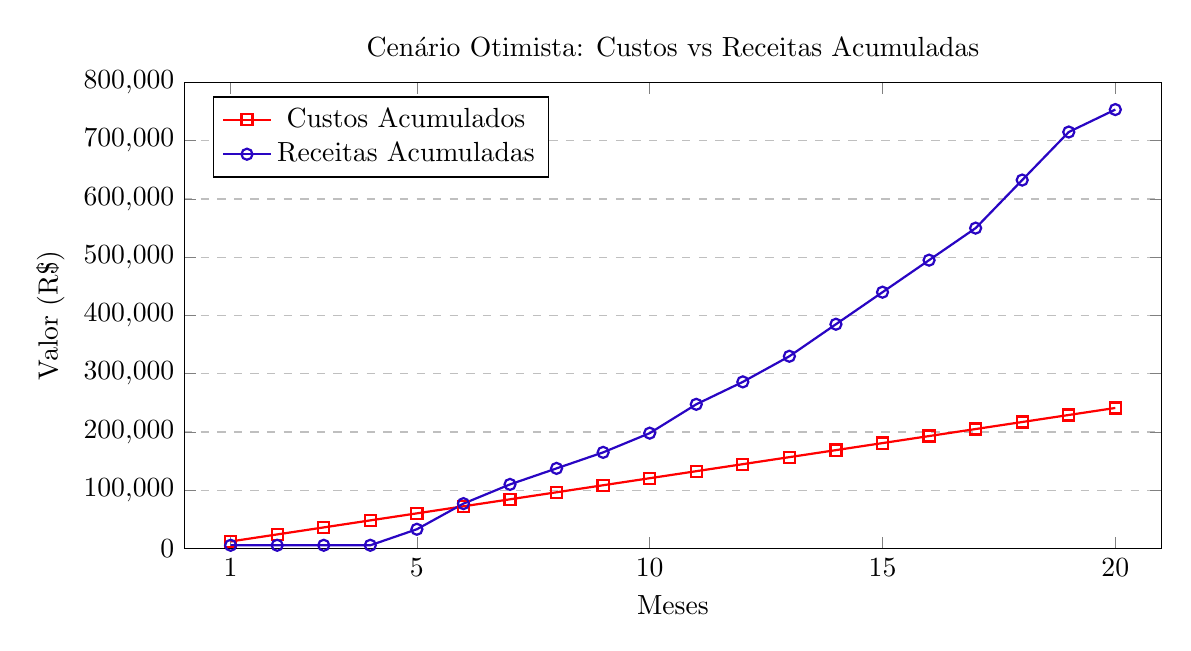
\begin{tikzpicture}
		\begin{axis}[
			title={Cenário Otimista: Custos vs Receitas Acumuladas},
			xlabel={Meses},
			ylabel={Valor (R\$)},
			xmin=0, xmax=21,
			ymin=0, ymax=800000,
			xtick={1,5,10,15,20},
			ytick={0,100000,200000,300000,400000,500000,600000,700000,800000},
			legend pos=north west,
			ymajorgrids=true,
			grid style=dashed,
			width=14cm,
			height=7.5cm,
			scaled y ticks = false,
			ticklabel style={/pgf/number format/fixed},
			]
			
			% Dados Custos Acumulados
			\addplot[
			color=red,
			mark=square,
			thick,
			]
			coordinates {
				(1,12062.46)
				(2,24124.92)
				(3,36187.38)
				(4,48249.84)
				(5,60312.30)
				(6,72374.76)
				(7,84437.22)
				(8,96499.68)
				(9,108562.14)
				(10,120624.60)
				(11,132687.06)
				(12,144749.52)
				(13,156811.98)
				(14,168874.44)
				(15,180936.90)
				(16,192999.36)
				(17,205061.82)
				(18,217124.28)
				(19,229186.74)
				(20,241249.20)
			};
			
			% Dados Receitas Acumuladas
			\addplot[
			color=blue,
			mark=o,
			thick,
			]
			coordinates {
				(1,5500)
				(2,5500)
				(3,5500)
				(4,5500)
				(5,33000)
				(6,77000)
				(7,110000)
				(8,137500)
				(9,165000)
				(10,198000)
				(11,247500)
				(12,286000)
				(13,330000)
				(14,385000)
				(15,440000)
				(16,495000)
				(17,550000)
				(18,632500)
				(19,715000)
				(20,753500)
			};
			
			\legend{Custos Acumulados, Receitas Acumuladas}
		\end{axis}
	\end{tikzpicture}
	\caption{Comparação dos custos e receitas acumuladas no cenário otimista}
	\fonte{Elaborado pelos autores.}
	\label{fig:custo-receita-otimista}
\end{figure}
\subsection{Cenário Pessimista}
Na \autoref{fig:custo-receita-pessimista} é possível observar a projeção construída pela equipe de um cenário pessimista, levando em consideração os custos já apresentados anteriormente de mão de obra e estrutura. De acordo com essa projeção, o ponto de equilíbrio será alcançado por volta de 20 meses.
\begin{figure}[H]
	\centering
	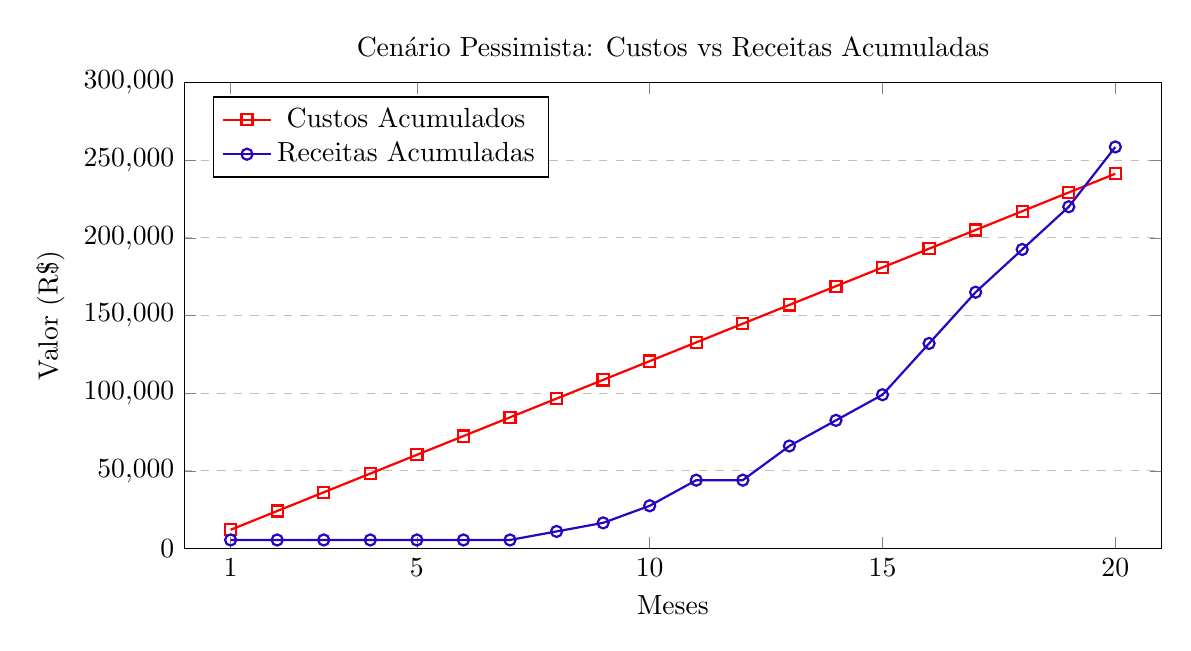
\begin{tikzpicture}
		\begin{axis}[
			title={Cenário Pessimista: Custos vs Receitas Acumuladas},
			xlabel={Meses},
			ylabel={Valor (R\$)},
			xmin=0, xmax=21,
			ymin=0, ymax=300000,
			xtick={1,5,10,15,20},
			ytick={0,50000,100000,150000,200000,250000,300000},
			legend pos=north west,
			ymajorgrids=true,
			grid style=dashed,
			width=14cm,
			height=7.5cm,
			scaled y ticks = false,
			ticklabel style={/pgf/number format/fixed},
			]
			
			% Dados Custos Acumulados
			\addplot[
			color=red,
			mark=square,
			thick,
			]
			coordinates {
				(1,12062.46)
				(2,24124.92)
				(3,36187.38)
				(4,48249.84)
				(5,60312.30)
				(6,72374.76)
				(7,84437.22)
				(8,96499.68)
				(9,108562.14)
				(10,120624.60)
				(11,132687.06)
				(12,144749.52)
				(13,156811.98)
				(14,168874.44)
				(15,180936.90)
				(16,192999.36)
				(17,205061.82)
				(18,217124.28)
				(19,229186.74)
				(20,241249.20)
			};
			% Dados Receitas Acumuladas
			\addplot[
			color=blue,
			mark=o,
			thick,
			]
			coordinates {
				(1,5500)
				(2,5500)
				(3,5500)
				(4,5500)
				(5,5500)
				(6,5500)
				(7,5500)
				(8,11000)
				(9,16500)
				(10,27500)
				(11,44000)
				(12,44000)
				(13,66000)
				(14,82500)
				(15,99000)
				(16,132000)
				(17,165000)
				(18,192500)
				(19,220000)
				(20,258500)
			};
			
			\legend{Custos Acumulados, Receitas Acumuladas}
		\end{axis}
	\end{tikzpicture}
	\caption{Comparação dos custos e receitas acumuladas no cenário pessimista}
	\fonte{Elaborado pelos autores.}
	\label{fig:custo-receita-pessimista}
\end{figure}
\subsection{Cenário Realista}
Na \autoref{fig:custo-receita-realista} é possível observar a projeção construída pela equipe de um cenário realista, levando em consideração os custos já apresentados anteriormente de mão de obra e estrutura. De acordo com essa projeção, o ponto de equilíbrio será alcançado por volta de 15 meses.
\begin{figure}[H]
	\centering
	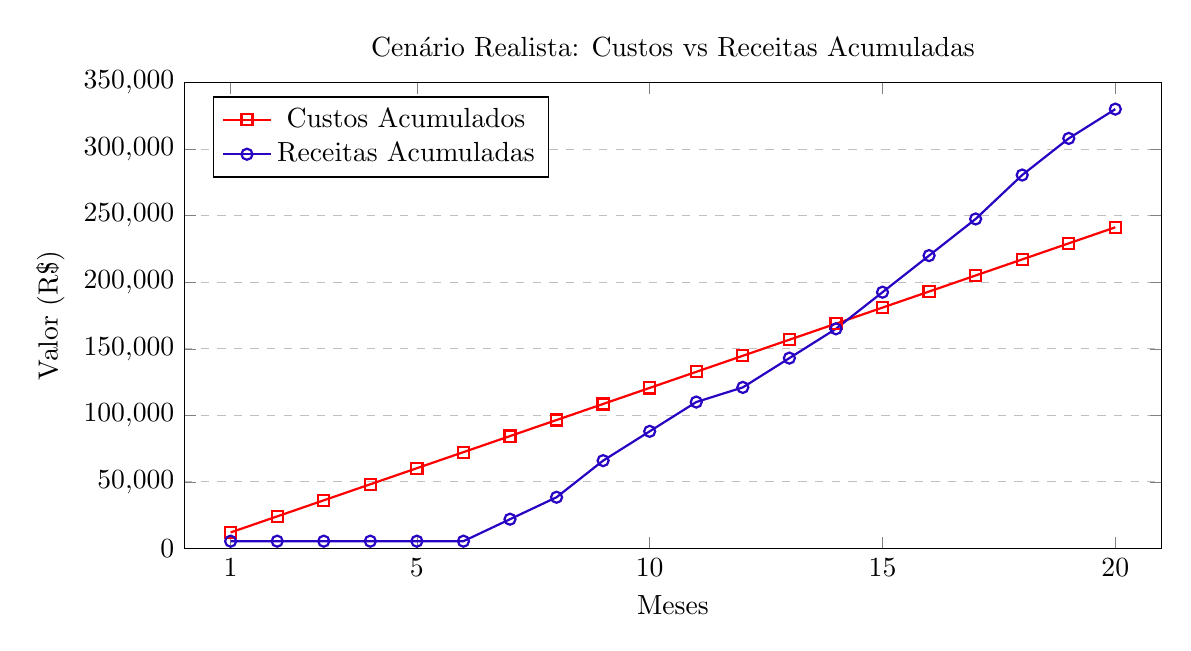
\begin{tikzpicture}
		\begin{axis}[
			title={Cenário Realista: Custos vs Receitas Acumuladas},
			xlabel={Meses},
			ylabel={Valor (R\$)},
			xmin=0, xmax=21,
			ymin=0, ymax=350000,
			xtick={1,5,10,15,20},
			ytick={0,50000,100000,150000,200000,250000,300000,350000},
			legend pos=north west,
			ymajorgrids=true,
			grid style=dashed,
			width=14cm,
			height=7.5cm,
			scaled y ticks = false,
			ticklabel style={/pgf/number format/fixed},
			]
			
			% Dados Custos Acumulados
			\addplot[
			color=red,
			mark=square,
			thick,
			]
			coordinates {
				(1,12062.46)
				(2,24124.92)
				(3,36187.38)
				(4,48249.84)
				(5,60312.30)
				(6,72374.76)
				(7,84437.22)
				(8,96499.68)
				(9,108562.14)
				(10,120624.60)
				(11,132687.06)
				(12,144749.52)
				(13,156811.98)
				(14,168874.44)
				(15,180936.90)
				(16,192999.36)
				(17,205061.82)
				(18,217124.28)
				(19,229186.74)
				(20,241249.20)
			};
			
			% Dados Receitas Acumuladas
			\addplot[
			color=blue,
			mark=o,
			thick,
			]
			coordinates {
				(1,5500)
				(2,5500)
				(3,5500)
				(4,5500)
				(5,5500)
				(6,5500)
				(7,22000)
				(8,38500)
				(9,66000)
				(10,88000)
				(11,110000)
				(12,121000)
				(13,143000)
				(14,165000)
				(15,192500)
				(16,220000)
				(17,247500)
				(18,280500)
				(19,308000)
				(20,330000)
			};
			
			\legend{Custos Acumulados, Receitas Acumuladas}
		\end{axis}
	\end{tikzpicture}
	\caption{Comparação dos custos e receitas acumuladas no cenário realista}
	\fonte{Elaborado pelos autores.}
	\label{fig:custo-receita-realista}
\end{figure}

\end{comment}

\chapter{Considerações Finais}

O desenvolvimento do sistema web para a pousada Chalés Água de Coco representa uma resposta prática e eficiente à necessidade de modernização enfrentada por pequenos empreendimentos do setor de hospitalidade. Ao longo do projeto, foi possível identificar fragilidades nos métodos tradicionais utilizados para gestão de hóspedes, reservas e finanças — especialmente aqueles baseados em planilhas eletrônicas — que, embora populares, oferecem baixa escalabilidade, alto risco de erro e pouca integração entre processos.

Através de uma parceria direta com os responsáveis pela pousada, foi possível realizar um levantamento detalhado dos requisitos do sistema, o que permitiu construir uma solução personalizada, centrada nas reais necessidades operacionais do negócio. O uso do \textit{framework} Django, aliado à infraestrutura da Amazon Web Services (AWS), proporcionou uma arquitetura robusta, segura e escalável, capaz de sustentar a aplicação tanto em seu estágio inicial quanto em futuras evoluções.

Além da automatização das principais funções administrativas da pousada, como o controle de reservas e a organização dos dados financeiros, o sistema promoveu melhorias significativas na usabilidade, no acesso remoto às informações e na geração de relatórios gerenciais. Com isso, o projeto atendeu plenamente aos seus objetivos, oferecendo uma ferramenta funcional, acessível via internet e com grande potencial de impacto na rotina de trabalho da pousada.

O projeto também demonstrou, na prática, a aplicabilidade dos conhecimentos adquiridos ao longo do curso, abrangendo aspectos de análise de requisitos, modelagem de dados, desenvolvimento \textit{back-end} e \textit{front-end}, segurança da informação e implantação em ambiente de nuvem. Trata-se, portanto, de um produto tecnológico que, além de resolver uma demanda real, reforça a importância da tecnologia na transformação digital de pequenos negócios.


%
% ----------------------------------------------------------
% Finaliza a parte no bookmark do PDF
% para que se inicie o bookmark na raiz
% e adiciona espaço de parte no Sumário
% ----------------------------------------------------------
\phantompart

% ---
% Conclusão
% ---
\chapter{Conclusão}
% ---

Este Projeto de Conclusão de Curso teve como propósito desenvolver um sistema \textit{web} para automatizar os processos administrativos da pousada Chalés Água de Coco, promovendo uma solução moderna e eficiente em substituição ao modelo tradicional baseado em planilhas. O sistema entregue oferece recursos essenciais para a gestão de hóspedes, reservas, acomodações e controle financeiro, consolidando-se como uma plataforma completa e adaptada à realidade da pousada.

A aplicação da arquitetura MTV com o \textit{framework} Django, a adoção de práticas seguras de desenvolvimento e o uso da infraestrutura em nuvem da AWS contribuíram para a construção de um sistema robusto e escalável, capaz de oferecer alto desempenho e disponibilidade. A utilização de tecnologias amplamente reconhecidas no mercado assegura não apenas a qualidade técnica do sistema, mas também sua viabilidade para expansão futura.

Como resultado, a pousada passa a contar com uma ferramenta que facilita a tomada de decisões, minimiza falhas operacionais e melhora a organização das informações. O projeto também evidencia como soluções de baixo custo e alto impacto podem ser desenvolvidas e aplicadas em pequenos negócios, promovendo inovação e melhoria contínua.


% ----------------------------------------------------------
% ELEMENTOS PÓS-TEXTUAIS
% ----------------------------------------------------------
\postextual
% ----------------------------------------------------------

% ----------------------------------------------------------
% Referências bibliográficas
% ----------------------------------------------------------
\bibliographystyle{abntex2-alf}
\bibliography{referencias}

% ----------------------------------------------------------
% Glossário
% ----------------------------------------------------------
%
% Consulte o manual da classe abntex2 para orientações sobre o glossário.
%
%\glossary

% ----------------------------------------------------------
% Apêndices
% ----------------------------------------------------------

% ---
% Inicia os apêndices
% ---
\begin{apendicesenv}

% Imprime uma página indicando o início dos apêndices
\partapendices

% ----------------------------------------------------------
\chapter{Diário de Bordo}
% ----------------------------------------------------------


\section{1° SEMANA}
Período: 25/03/2025 a 01/04/2025.

Nessa semana, com os membros da equipe definidos, iniciamos nossas atividades para o desenvolvimento do projeto da disciplina de Projeto de Extensão Integrado I. Assim, essa semana criamos um grupo na plataforma Whatsapp para estabelecermos nossa comunicação e facilitar o levantamento de possíveis temas para discutirmos em sala. Assim, no dia 01/04/2025 analisamos os parceiros disponíveis e a suas principais necessidades e optamos por desenvolver uma aplicação web para a empresa Pousada Chalés Água de Coco. 

\section{2° SEMANA}
Período: 01/04/2025 a 08/04/2025.

Durante essa semana aprofundamos nosso conhecimento sobre a empresa parceira escolhida, entendo sua principal necessidade: automatização dos serviços de gestão.
Definimos que iremos desenvolver uma aplicação web de gestão para a proprietária com o objetivo de facilitar e otimizar a administração do negócio. A partir disso, também definimos nosso MVP (Produto Mínimo Viável), levando em consideração nossa capacidade técnica e os serviços da pousada. Preenchemos a primeira planilha de avaliação do grupo e auto-avaliação. Por fim, nos preparamos para apresentar a nossa escolha de tema para o professor orientador, realizada no dia 08/04, na qual também apresentamos nosso MVP.
Funcionalidade MVP: Gestão de Reservas e Check-in/Check-out. 	


\section{3° SEMANA}
Período: 08/04/2025 a 15/04/2025.

Nesta semana começamos efetivamente as tarefas associadas ao desenvolvimento do nosso projeto. Foram elas:
	\begin{itemize}
		\item Definimos a metodologia de gestão de projeto Scrum. Usamos como base para  nossa escolha: experiências práticas/ conhecimento prévio da ferramenta, isto é, familiaridade. 
		\item Definimos a função de cada membro da equipe:
		\begin{itemize}
			\item Guilherme Akio: Analista de Testes.
			\item Guilherme Schmidt: Engenheriro de Software.
			\item Kelly Radchelle: Gerente de Projeto.
			\item Rafael Teixeira: Desenvolvedor Frontend.
			\item Ricardo Carriel: Desenvolvedor Backend.
			\item Criamos nosso arquivo no ProjectLibre, adicionamos os principais marcos do projeto e os recursos humanos.
			\item Criamos nossa documentação LateX e fizemos as primeiras alterações no arquivo.
			\item Iniciamos o levantamento dos requisitos funcionais do MVP.
		\end{itemize}
	\end{itemize}

\section{4° SEMANA}
Período: 15/04/2025 a 22/04/2025.

Nesta semana foram realizadas as tarefas e discussões para iniciarmos o desenvolvimento do desenho da nossa aplicação:
Analisamos os requisitos funcionais levantados e definimos os requisitos não funcionais essenciais da nossa aplicação.
E definimos as plataformas e tecnologias que iremos usar.


\section{5° SEMANA}
Período: 22/04/2025 a 29/04/2025.

Essa semana foram desenvolvidas atividades ligadas ao desenvolvimento da prova de conceito. Foram elas:
	\begin{itemize}
		\item Kelly Radchelle: Documentação dos Casos de Uso.
		\item Guilherme Schmidt: Documentação dos Diagramas de Caso de Uso.
		\item Reunião via Google Meet na qual foi discutido o desenho da aplicação com todos os membros da equipe.
		\item Guilherme Bittencourt: Criação do Diagrama de Componentes.
		\item Kelly Radchelle: Criação do Diagrama de Implantação.
		\item Guilherme Schmidt, Guilherme Akio, Rafael Teixeira e Ricardo Carriel: Apresentação do Desenho da Aplicação.
	\end{itemize}
\section{6° SEMANA}
Período: 29/04/2025 a 06/05/2025.

Após a entrega da prova de conceito na semana anterior os diagramas apresentados foram editados, corrigindo os pontos levantados 
pelo professor orientador. 
	\begin{itemize}
		\item Guilherme Schmidt: Alterações no diagrama de componentes. 
		\item Kelly Radchelle: Alterações no diagrama de implantação.
		\item Guilherme Schmidt: Criação do MER.
		\item Guilherme Schmidt: Criação do repositório Git para versionamento da aplicação.
		\item Kelly Radchelle e Ricardo Carriel: Levantamento das regras de negócio e requisitos com a proprietária.
	\end{itemize}
	

\section{7° SEMANA}
Período: 06/05/2025 a 13/05/2025.

Nesta semana foram realizadas atividades para a entrega da POC (Prova de Conceito). Foram elas:
	\begin{itemize}
		\item  Guilherme Akio: Início do desenvolvimento do backend e frontend no Django: views, models e templates.
		\item  Ricardo Carriel: Início da configuração do ambiente de hospedagem.
	\end{itemize}
	
Além de continuarmos com as atividades de documentação e alimentação do nosso repositório Git.

\section{8° SEMANA}
Período: 13/05/2025 a 20/05/2025.

Nessa semana o Ricardo e o Guilherme Akio finalizaram a integração entre o ambiente de hospedagem, criação do banco de dados no postgreSQL e o servidor Django. 
Assim, conseguimos finalizar, entregar e apresentar a prova de conceito. Além disso, aproveitamos para revisar os nossos requisitos e  regras de negócio e 
estruturamos de forma mais completa nossos requisitos não funcionais.

\section{9° SEMANA}
Período: 20/05/2025 a 27/05/2025.

Nesta semana demos continuidade ao desenvolvimento do nosso MVP, focando agora nas funcionalidades e interfaces. Alimentamos nosso repositório git com arquivos referentes a documentação.
	\begin{itemize}
		\item Ricardo Carriel: Atualizações no código. .
		\item Kelly Radchelle: Desenvolvimento da Documentação.
		\item Guilherme Schmidt: Desenvolvimento da Documentação.
	\end{itemize}


\section{10° SEMANA}
Período: 27/05/2025 a 03/06/2025.

Nesta semana os esforços da equipe foram voltados para o desenvolvimento e consolidação da documentação do projeto. 
Dessa forma, todos os integrantes tiveram como atividade a documentação e revisão de algum aspecto do sistema.  Além disso, o
integrante Rafael fez correções na extensão HTML.

\section{11° SEMANA}
Período: 03/06/2025 a 10/06/2025.

Nesta semana o foco da equipe se manteve em desenvolver e revisar os tópicos da documentação.
Responsabilidades de cada integrante:
	\begin{itemize}
		\item Guilherme Akio: Documentação do código e das funcionalidades desenvolvidas por si. 
		\item Guilherme Schmidt: Entregar seus tópicos da documentação (Introdução, Manutenabilidade, Segurança e Privacidade e Arquitetura do Sistema) e auxiliar na revisão e desenvolvimento da Documentação.
		\item Kelly Radchelle: Entregar seus tópicos da documentação (Gestão do Projeto,  Escopo do Projeto e Histórias de Usuário) e auxiliar na revisão e desenvolvimento da documentação final.
		\item Rafael Teixeira: Documentação do código e das funcionalidades desenvolvidas por si.
	\end{itemize}
\section{12° SEMANA}
Período: 10/06/2025 a 17/06/2025.

Nesta semana a equipe corrigiu e revisou os tópicos da documentação e realizou alterações na estrutura do código para corrigir erros e facilitar o entendimento do mesmo. Além de, corrigir erros recorrentes no ProjectLibre.

\section{13° SEMANA}
Período: 17/06/2025 a 24/06/2025.

Durante essa semana a documentação final consolidada foi revisada, para aplicar aspectos faltantes das normas abnt. Desenvolveu as funcionalidades restantes relacionadas ao módulo de reserva e check-in/check-out. E iniciou os preparativos para a apresentação final do MVP.

\section{Período: 13/08/2025 a 26/08/2025.}
Durante esse período de retorno as atividades do projeto, fizemos a revisão dos requisitos e regras de negócio finais do sistema,
com o objetivo de planejar as sprints da segunda fase do projeto. Levantamos funcionalidades essenciais e que ficaram pendentes da 
primeira fase. Definimos a nova ferramenta para acompanhamento das atividades (Github - Project) das sprints e como seriam dividas
as issues/tasks. 

\section{14° SEMANA}
Período: 27/08/2025 a 02/09/2025.
Durante a primeira sprint da segunda fase do projeto, foram planejadas atividades de revisão e retomada de funcionalidades
pendentes do sistema e planejamento do plano de testes: 
	\begin{itemize}
		\item Rafael Teixeira:  Adicionar campo de motivo de cancelamento de reserva. 	
		\item Rafael Teixeira: Criar função de editar cadastro de quartos .	
		\item Guilherme Schimdt: Revisar e Corrigir tópico Introdução. 
		\item Guilherme Schimdt: Revisar e corrigir o tópico objetivo.
		\item Kelly Radchelle: Revisar e ajustar product backlog.
		\item Kelly Radchelle: Revisar e atualizar o escopo do projeto.
		\item Ricardo Carriel: Revisar e padronizar código.	
		\item Guilherme Akio: Criar estrutura do plano de teste.
	\end{itemize}	

\section{15° SEMANA}
Período: 03/09/2025 a 10/09/2025.
Nesta semana foi iniciado o desenvolvimento e implementação de novas funcionalidades relacionadas ao módulo financeiro. As atividades foram distribuídas:
	\begin{itemize}	
		\item Rafael Teixeira: Criar tabela financeiro\_título.
		\item Ricardo Carriel: Criar app Financeiro com configurações iniciais. 
		\item Kelly Radchelle: Revisar e atualizar tópico histórias de usuário.
		\item Kelly Radchelle: Atualizar tópico de Sprint Backlog.
		\item Guilherme Schimdt: Revisar e Corrigir Justificativa.
		\item Guilherme Schimdt: Revisar e corrigir tópico de Análise da concorrência.
		\item Guilherme Akio: Testar módulo de gestão de hóspedes.
	\end{itemize}
	
\section{16° SEMANA}
Período: 11/09/2025 a 17/09/2025.
Durante a semana foi planejado realizar novas implementações no módulo financeiro e de autenticação. s 
atividades foram distribuídas:
	\begin{itemize}
		\item Rafael Teixeira: Criar tabela financeiro\_categoria.
		\item Guilherme Schimdt: Revisar e corrigir tópico de Modelagem do banco de dados.
		\item  Kelly Radchelle: Revisar e corrigir tópico de gestão do projeto.
		\item Kelly Radchelle: Implementar login/logout.	
		\item Ricardo Carriel: Criar tabela financeiro\_banco.
		\item Guilherme Akio: Realizar testes no módulo gestão de reservas. 
	\end{itemize}
Além disso,  foram revistos os requisitos funcionais finais com a empresa parceira.

\section{17° SEMANA}
Período: 18/09/2025 a 24/09/2025.
Para a sprint dessa semana foram planejadas as tarefas:
	\begin{itemize}
		\item Rafael Teixeira: Criar views de CRUD para Títulos.
		\item Rafael Teixeira: Ajuste - Adicionar campo de motivo de cancelamento de reserva.	
		\item Guilherme Akio: Realizar testes no módulo gestão de quartos.	
		\item Ricardo Carriel: Implementar integração com módulo de reservas.
		\item Guilherme Schimdt: Revisar e corrigir tópico de Segurança .
		\item Guilherme Schimdt: Realizar testes funcionais módulo de gestão de hóspedes.
		\item Kelly Radchelle: Revisar e Corrigir Revisão de Literatura.
		\item Kelly Radchelle: Criar telas de autenticação.
	\end{itemize}
	
\section{18° SEMANA}
Período: 25/09/2025 a 01/10/2025.
Para a sprint dessa semana foram planejadas as tarefas:
	\begin{itemize}
	\item Rafael Teixeira: Criar filtros para lista de reservas.
	\item Rafael Teixeira: Implementar cadastro de categorias de despesa.
	\item Kelly Radchelle: Criar função de envio de e-mail de confirmação de reserva.
	\item Guilherme Schimdt: Realizar testes funcionais módulo de gestão de quartos.
	\item Guilherme Akio: Realizar ajustes módulo hóspedes. 
	\item Guilherme Schimdt: Revisar e corrigir a Arquitetura do projeto.
	\item Guilherme Schimdt: Realizar testes funcionais módulo de gestão de reservas.
	\item Ricardo Carriel: Criar funcionalidade de baixa do pagamento.
	\item Ricardo Carriel: Implementar regra de pagamento parcial para confirmação da reserva.
	\item Kelly Radchelle: Revisar e corrigir tópico de Viabilidade financeira .
	\end{itemize}
	
\section{19° SEMANA}
Período: 02/10/2025 a 08/10/2025.
Para a sprint dessa semana foram planejadas as tarefas:
	\begin{itemize}
		\item Guilherme Akio: Testes de funcionais de autenticação. 
		\item Guilherme Akio: Criar filtros por categoria para títulos.
		\item Rafael Teixeira: Criar view de balanço financeiro.
		\item Rafael Teixeira: Criar pacotes de reservas.	
		\item Guilherme Schimdt: Revisar e corrigir tópico de Tecnologias e ferramentas de apoio utilizadas. 
		\item Guilherme Schimdt: Realizar testes unitários do CRUD de títulos. 
		\item Ricardo Carriel: Criar funcionalidade de adição de tarifas à reserva.
		\item Ricardo Carriel: Criar templates de título. 
		\item Kelly Radchelle: Realizar ajustes no módulo quarto.
		\item Kelly Radchelle: Realizar ajustes módulo de reservas.
	\end{itemize}
E envio do documento de requisitos funcionais finais para a empresa parceira e para o professor orientador.

\section{20° SEMANA}
Período: 09/10/2025 a 15/10/2025.
Para a sprint dessa semana foram estipuladas as tarefas:
	\begin{itemize}
		\item Rafael Teixeira: Criar view do painel de métricas.
		\item Ricardo Carriel: Criar templates para tarifas.
		\item Guilherme Akio: Criar view relatórios: financeiro.
		\item Guilherme Schimdt: Revisão e atualização dos diagramas.
		\item Kelly Radchelle: Criar view relatórios: ocupação.
	\end{itemize}
	
\section{21° SEMANA}
Período: 16/10/ 2025 a 22/10/2025.
Para a sprint dessa semana foram estipuladas as tarefas:
	\begin{itemize}
		\item Rafael Teixeira: Criar template: painel de métricas.
		\item Guilherme Schimdt: Adicionar tópico de estilo de código na documentação.
		\item Kelly Radchelle: Criar template relatório de ocupação.
		\item Guilherme Akio: Criar template relatórios financeiros.
		\item Ricardo Carriel: Configurar envio de email no servidor AWS.
	\end{itemize}
	
\section{22° SEMANA} 
Período: 23/10/2025 a 29/10/2025.
Para a sprint dessa semana foram determinadas as tarefas:
	\begin{itemize}
		\item Kelly Radchelle: Ajustar e padronizar templates. 
		\item Guilherme Schimdt: Realizar testes funcionais: títulos.
		\item Guilherme Akio: Adicionar lógica de disponibilidade de quartos.
		\item Ricardo Carriel: Adicionar  função de early check-in e late check-out.
		\item Rafael Teixeira: Criar funcionalidade de notificação.
	\end{itemize}
	
\section{23° SEMANA}
Período: 30/10/2025 a 5/11/2025.
Essa semana foi separada para realização de novos testes e para finalização de issues não finalizadas, a fim de 
conseguir fazer a entrega do produto final (prevista para o dia 12/11). Foram elas:
	\begin{itemize}
		\item Guilherme Schimdt: Revisar e Realizar testes unitários. (Responsável: )
		\item Kelly Radchelle: Revisar e corrigir tópico de Repositório da Aplicação. 
		\item Guilherme Akio: Finalizar issues sob responsabilidade própria em atraso.
		\item Rafael Teixeira: Finalizar issues sob responsabilidade própria em atraso.
		\item Ricardo Carriel: Finalizar issues sob responsabilidade própria em atraso.
	\end{itemize}
	
\section{24° SEMANA} 
Período: 30/10/2025 a 11/5/2025.
Durante essa semana foi dado continuidade a tarefas não finalizadas e novos testes unitários. Além da revisão final da 
documentação.

% ----------------------------------------------------------
\chapter{Questionário Aplicado à Proprietária da Pousada}
\label{apendice:questionario1}
\section{Questionário 1: Levantamento de Requisitos}
O \autoref{quadro:questionario1} foi aplicado à proprietária da pousada parceira para a análise e levantamento dos requisitos do sistema.

\begin{quadro}[H]
	\caption{Questionário Aplicado à Proprietária 1 (Parte 1)}
	\label{quadro:questionario1}
	\vspace{0.3cm} 
	\begin{tabular}{|>{\centering\arraybackslash}p{1cm}|p{6.5cm}|p{6.5cm}|}
		\hline
		\multicolumn{3}{|l|}{\textbf{Domínio: Reservas}} \\ \hline
		\textbf{Item} & \textbf{Pergunta} & \textbf{Resposta} \\ \hline
		1 &  Como os clientes normalmente fazem uma reserva hoje (telefone, WhatsApp, pessoalmente)? & Geralmente, por WhatsApp. \\ \hline
		2 & Há um prazo mínimo ou máximo para fazer uma reserva? & Preferencialmente, antecipadamente. Nas plataformas coloco 2 dias de antecedência. \\ \hline
		3 & A reserva é confirmada apenas com pagamento ou pode ser feita sem pagamento antecipado? & Confirmada pelo pagamento de pelo menos metade do valor da reserva. \\ \hline
		4 & É permitido cancelar uma reserva? Até quantas horas antes do check-in? Há cobrança de taxa? & Sim! Temos políticas de cancelamentos e remarcações. \\ \hline
		5 & Um hóspede pode fazer mais de uma reserva ativa ao mesmo tempo? & Sim. \\ \hline
		\multicolumn{3}{|l|}{\textbf{Domínio: Hóspedes}} \\ \hline
		\textbf{Item} & \textbf{Pergunta} & \textbf{Resposta} \\ \hline
		6 & Quais dados do hóspede são obrigatórios para fazer uma reserva? & Nome completo, endereço completo, CPF, telefone, e-mail. \\ \hline
		7 & É comum ter reservas feitas por um responsável em nome de outros hóspedes? & Sim. \\ \hline
		8 & Há um limite de pessoas por quarto? Como isso é controlado? & No check-in. \\ \hline
	\end{tabular}
	\vspace{0.5cm}
	\fonte{Elaborado pelos autores.}
\end{quadro}
%
\begin{quadro}[H]
	\ContinuedFloat
	\caption{Questionário Aplicado à Proprietária 1 (Parte 2)}
	%\caption*{\quadroname~\ref{quadro:questionario1} – Questionário Aplicado à Proprietária 1 (Parte 2)}
	\vspace{0.3cm}
	\begin{tabular}{|>{\centering\arraybackslash}p{1cm}|p{6.5cm}|p{6.5cm}|}
		\hline
	
		\multicolumn{3}{|l|}{\textbf{Domínio: Check-in e Check-out}} \\ \hline
		\textbf{Item} & \textbf{Pergunta} & \textbf{Resposta} \\ \hline
		9 & Qual é o horário padrão de check-in e check-out? Há tolerância? & Check-in a partir das 16h até às 22h e check-out das 8h até às 14h. Depende de se há entrada de outro hóspede em seguida. \\ \hline
		10 & O check-in pode ser feito antes do horário? E o check-out após o horário? & Depende, se houver saída de hóspede anterior ou entrada em seguida. \\ \hline
		11 & Quem realiza o check-in e check-out? Você ou os funcionários? & Eu ou sozinhos, com orientações minhas. \\ \hline
		12 & Há necessidade de gerar comprovante ou recibo após check-in ou check-out? & Não. \\ \hline
			13 & A pousada possui quantos quartos? Como eles são classificados? & 16. Quartos simples simples para casal (com e sem ar), chalés com cozinha para até 4 pessoas, com e sem ar e flats, com e sem ar \\
		\hline
		14 & Há períodos em que quartos são bloqueados para manutenção ?& Sim\\
		\hline
		15 & Um mesmo quarto pode ser reservado para diferentes hóspedes em dias seguidos?& Sim. \\
		\hline
		\multicolumn{3}{|l|}{\textbf{Domínio: Serviços Adicionais}} \\ \hline
		\textbf{Item} & \textbf{Pergunta} & \textbf{Resposta} \\
		\hline
		16 &  A pousada oferece serviços extras? & Não. \\ 
		\hline
		17 & Se sim, esses serviços devem ser registrados no sistema junto à reserva? & (Não há serviços extras)\\
		\hline
		\multicolumn{3}{|l|}{\textbf{Domínio: Pagamentos}} \\
		\hline
		\textbf{Item} & \textbf{Pergunta} & \textbf{Resposta} \\ 
		\hline
		18 &  Quais formas de pagamento são aceitas (Pix, cartão, dinheiro)? & As três formas, porém no cartão tem taxa da operadora. \\
		\hline
		19 &  Os pagamentos são feitos no check-in, no check-out ou antecipadamente? & Metade na reserva e o restante na chegada.\\ 
		\hline
		20 &  É necessário gerar comprovante ou recibo no sistema? & Eu envio uma confirmação de reserva com todas as informações.\\ 
		\hline
	\end{tabular}
	\vspace{0.5cm}
	\fonte{Elaborado pelos autores.}
\end{quadro}
%
\begin{comment}
\begin{quadro}[H]
	\caption*{\quadroname~\ref{quadro:questionario1} – Questionário Aplicado à Proprietária (Parte 3)}
	\vspace{0.3cm} 
	\begin{tabular}{|>{\centering\arraybackslash}p{1cm}|p{6.5cm}|p{6.5cm}|}
		\hline
			\multicolumn{3}{|l|}{\textbf{Domínio: Quartos}} \\ \hline
		\textbf{Item} & \textbf{Pergunta} & \textbf{Resposta} \\
		\hline
	
	\end{tabular}
	\fonte{Elaborado pelos autores.}
\end{quadro}
\end{comment}
%

\begin{quadro}[H]
	\ContinuedFloat
	\caption{Questionário Aplicado à Proprietária 1 (Parte 3)}
	%\caption*{\quadroname~\ref{quadro:questionario1} – Questionário Aplicado à Proprietária 1 (Parte 3)}
	\vspace{0.3cm} 
	\begin{tabular}{|>{\centering\arraybackslash}p{1cm}|p{6.5cm}|p{6.5cm}|}
		\hline
	
		\multicolumn{3}{|l|}{\textbf{Domínio: Comunicação}} \\ \hline
		\textbf{Item} & \textbf{Pergunta} & \textbf{Resposta} \\ \hline
		21 & Você gostaria que o sistema enviasse confirmação automática de reserva por WhatsApp ou e-mail? & Sim. \\ \hline
		22 &  Há interesse em receber alertas automáticos de check-in, check-out ou cancelamento? & Sim. \\ \hline
		\multicolumn{3}{|l|}{\textbf{Domínio: Acesso ao Sistema}} \\
		\hline
		\textbf{Item} & \textbf{Pergunta} & \textbf{Resposta} \\ 
		\hline
		23 & Somente você vai usar o sistema ou os funcionários também? & Somente eu. \\
		\hline
		24 &  Deseja que cada pessoa tenha um tipo de acesso diferente? & (Somente a proprietária vai usar o sistema).\\ 
		\hline
		25 & O sistema será usado no computador, celular ou ambos? & Em ambos. \\ \hline
		\multicolumn{3}{|l|}{\textbf{Domínio: Relatórios e Controle}} \\ \hline
		\textbf{Item} & \textbf{Pergunta} & \textbf{Resposta} \\ \hline
		26 & Quais relatórios são mais importantes no dia a dia? & Ocupação diária, reservas da semana, totais de pagamento, período, …
		\\ \hline
		27 & É importante ter um histórico de cada hóspede e das reservas anteriores? & Sim. \\ 
		\hline
	\end{tabular}
	\vspace{0.5cm}
	\fonte{Elaborado pelos autores.}
\end{quadro}
\vspace{5cm}
% ------------------QUESTIONARIO 2---------------------------%
\section{Questionário 2: Viabilidade Financeira}
\label{apendice:questionario2}

O \autoref{quadro:questionario2_1} foi aplicado à proprietária da pousada parceira para a análise da viabilidade financeira do projeto

%
\begin{quadro}[H]
	\caption{Questionário Aplicado à Proprietária 2}
	\label{quadro:questionario2_1}
	\vspace{0.3cm}
	\begin{tabular}{|>{\centering\arraybackslash}p{1cm}|p{6.5cm}|p{6.5cm}|}
		\hline
		\textbf{Item} & \textbf{Pergunta} & \textbf{Resposta} \\ \hline
		1 & Pensando em uma reserva de diária (do primeiro contato até enviar a confirmação), quanto tempo você leva em média para fazer tudo? & Tudo depende do cliente, às vezes a demora ocorre pela indecisão ou espera de outros orçamentos por
		parte dele. Assim que o hóspede efetua o pagamento eu já envio a confirmação\\ \hline
		2 & E quantas reservas de diária você gerencia por mês, mais ou menos? & Depende também da época do ano e do tempo (clima), por ser na praia. Não são muitos pq tenho poucos disponíveis devido aos mensalistas, mas esse mês umas 15 diárias.\\ \hline
		3 & Em média, quantos hóspedes mensalistas você costuma ter? & No momento estou com 10 mensalistas. \\ \hline
		4 & Todo mês, quanto tempo você gasta para gerenciar o pagamento de cada mensalista? & Os dias não são geralmente os mesmos, por isso não leva tanto tempo. \\ \hline
		5 & No fim do mês, quantas horas você leva para fazer o fechamento financeiro? & No fim do mês fico bem atarefada por que deixo para emitir as NF, fazer fechamento financeiro, administrar RH, pagamentos, etc. \\ \hline
		6 & Pensando em erros de agendamento (overbooking): Isso já aconteceu no último ano por ser no controle manual? & Como sou bem organizada e só eu cuido disso, não aconteceu comigo pq faço vários registros. \\ \hline
		7 & Hoje, se eu te pedisse a taxa de ocupação de 6 meses atrás, seria fácil saber? & Seria fácil porque estávamos na baixa temporada e a taxa de ocupação é baixa, em média uns 5\%. \\ \hline
	\end{tabular}
	\vspace{0.5cm}
	\fonte{Elaborado pelos autores.}
\end{quadro}
% ----------------------------------------------------------%
\FloatBarrier
\clearpage
\phantomsection
\chapter{Product Backlog Detalhado}
\label{apendice:productbacklogcomp}
%
\begin{quadro}[H]
	\caption{Product Backlog Detalhado (Parte 1)}
	\label{quadro:product_backlog}
	\begin{tabular}{|>{\centering\arraybackslash}m{1.4cm}|>{\arraybackslash}m{6.5cm}|>{\centering\arraybackslash}m{3.8cm}|>{\centering\arraybackslash}m{2.5cm}|}
		\hline
		\textbf{Código} & 
		\multicolumn{1}{>{\centering\arraybackslash}m{6.5cm}|}{\textbf{Item}} &
		\textbf{Categoria} &
		\textbf{Prioridade} 
		\\ \hline
		1 & Definir e configurar ambiente de desenvolvimento & Requisito Técnico   & ALTA    \\ \hline
		2 & Definir ambiente de hospedagem/publicação & Requisito Técnico & ALTA  \\ \hline
		3 & Organizar repositório e fluxo Git  & Requisito Técnico & ALTA\\ \hline
		4 & Levantar requisitos funcionais e não funcionais    & Modelagem de dados & ALTA    \\ \hline
		5 & Mapear casos de uso & Modelagem de dados   & ALTA  \\ \hline
		6 & Documentar o levantamento e registrar os requisitos    & Documentação   & ALTA    \\ \hline
		7 & Criar Modelo Entidade-Relacionamento (MER)    & Modelagem de dados   & ALTA    \\ \hline
		8 & Criar Diagrama de Entidade-Relacionamento (DER)    & Modelagem de dados   & ALTA    \\ \hline
		9 & Criar Diagrama de Componentes    & Arquitetura   & ALTA    \\ \hline
		10 & Criar Diagrama de Implantação    & Arquitetura   & ALTA    \\ \hline
		11 & Documentar os diagramas produzidos & Documentação &
		ALTA \\ \hline
		12 & Configurar ambiente do servidor & Requisito Técnico &
		ALTA \\ \hline
		13 & Configurar banco de dados PostgreSQL & Requisito Técnico &
		ALTA \\ \hline
		14 & Implementar login e logout de usuário & Autenticação e Segurança & ALTA \\ \hline
		15 & Criar funcionalidades de cadastro de quartos & Gestão de Quartos & ALTA \\ \hline
		16 & Criar funcionalidade de exclusão de cadastro de quartos &
		Gestão de Quartos & MÉDIA \\ \hline
		17 & Criar funcionalidade de listagem de quartos & Gestão de Quartos & MÉDIA \\ \hline
		18 & Criar funcionalidade de edição do cadastro de quartos &
		Gestão de Quartos &	MÉDIA \\ \hline
	\end{tabular}
	\vspace{0.5cm}
	\fonte{Elaborado pelos autores.}
\end{quadro}
%
\begin{quadro}[H]
	\ContinuedFloat
	\caption{Product Backlog Detalhado (Parte 2)}
	%\caption*{\quadroname~\ref{quadro:product_backlog} – Product Backlog (Parte 2)}
	\begin{tabular}{|>{\centering\arraybackslash}m{1.4cm}|>{\arraybackslash}m{6.5cm}|>{\centering\arraybackslash}m{3.8cm}|>{\centering\arraybackslash}m{2.5cm}|}
		\hline
		\textbf{Código} & 
		\multicolumn{1}{>{\centering\arraybackslash}m{6.5cm}|}{\textbf{Item}} &
		\textbf{Categoria} &
		\textbf{Prioridade} 
		\\ \hline
		19 & Criar interfaces para gestão de quartos & Gestão de Quartos & MÉDIA \\ \hline
		20 & Implementar funcionalidade de alteração manual do status (disponível, indisponível, em manutenção) do quarto & Gestão de Quartos & MÉDIA \\ \hline
		21 & Criar funcionalidade de cadastro de hóspedes &	Gestão de Hóspedes & ALTA \\ \hline
		22 & Criar funcionalidade de exclusão do cadastro de hóspedes &
		Gestão de Hóspedes & MÉDIA \\ \hline
		23 & Criar funcionalidade de edição do cadastro de hóspedes &
		Gestão de Hóspedes & MÉDIA \\ \hline
		24 & Criar interfaces para gestão de hóspedes &	Gestão de Hóspedes & MÉDIA \\ \hline
		25 & Criar funcionalidade de cadastro de reservas &	Gestão de Reservas & ALTA \\ \hline
		26 & Criar funcionalidade de exclusão do cadastro de reservas &
		Gestão de Reservas & ALTA \\ \hline
		27 & Criar funcionalidade de edição do cadastro de reservas &
		Gestão de Reservas & ALTA \\ \hline
		28 & Criar interfaces para gestão de Reservas &	Gestão de Reservas & ALTA \\ \hline
		29 & Criar funcionalidade para visualização do histórico de reservas por hóspede & Gestão de Reservas &	MÉDIA \\ \hline
		30 & Criar lógica de validação de disponibilidade de quartos para reservas & Gestão de Reservas & ALTA \\ \hline
		31 & Implementar atualização automática do status do quarto para “ocupado” após o \textit {check-in} & \textit {Check-in} e \textit {Check-out} & ALTA 
		\\ \hline
		32 & Criar funcionalidade de atualização do \textit {check-out} &
		\textit {Check-in} e \textit {Check-out} &	ALTA \\ \hline
		33 & Integrar ambientes, \textit{backend} e \textit {frontend} &	Requisito técnico & ALTA \\ \hline
		34 & Documentar a configuração e o código desenvolvido &
		Documentação & ALTA \\ \hline
		35 & Criar funcionalidade de cadastro de receitas &	Gestão Financeira & BAIXA \\ \hline
	\end{tabular}
	\vspace{0.5cm}
	\fonte{Elaborado pelos autores.}
\end{quadro}
% 
\begin{quadro}[H]
	\ContinuedFloat
	\caption{Product Backlog Detalhado (Parte 3)}
	%\caption*{\quadroname~\ref{quadro:product_backlog} – Product Backlog (Parte 3)}
	\begin{tabular}{|>{\centering\arraybackslash}m{1.4cm}|>{\arraybackslash}m{6.5cm}|>{\centering\arraybackslash}m{3.8cm}|>{\centering\arraybackslash}m{2.5cm}|}
		\hline
		\textbf{Código} & 
		\multicolumn{1}{>{\centering\arraybackslash}m{6.5cm}|}{\textbf{Item}} &
		\textbf{Categoria} &
		\textbf{Prioridade} 
		\\ \hline
		36 & Criar funcionalidade para registrar comprovação de pagamento de reservas &	Gestão Financeira/Gestão de Reservas &
		BAIXA \\ \hline
		37 & Criar funcionalidade de exclusão do cadastro de receitas &
		Gestão Financeira &	BAIXA \\ \hline
		38 & Criar funcionalidade de edição do cadastro de receitas &
		Gestão Financeira &	BAIXA \\ \hline
		39 & Criar interface para gestão de receitas & Gestão Financeira & BAIXA \\ \hline
		40 & Criar funcionalidade de cadastro de despesas &
		Gestão Financeira & BAIXA \\ \hline
		41 & Criar funcionalidade de exclusão do cadastro de despesas &
		Gestão Financeira &	BAIXA \\ \hline
		42 & Criar funcionalidade de edição do cadastro de despesas &
		Gestão Financeira &	BAIXA \\ \hline   
		43 & Criar interface para gestão de despesas & Gestão Financeira & BAIXA \\ \hline
		44 & Criar funcionalidade para criar relatórios de quartos &
		Gestão Financeira &	BAIXA \\ \hline
		45 & Criar funcionalidade para criar relatórios de hóspedes &
		Gestão Financeira &	BAIXA \\ \hline
		46 & Criar funcionalidade para criar relatórios de reservas &
		Gestão Financeira &	BAIXA \\ \hline
		47 & Criar balanço financeiro simples (receitas, despesas, saldo) por período & Gestão Financeira & BAIXA \\ \hline
		48 & Criar funcionalidade de filtragem de receita/despesa (data, categoria) &	Gestão Financeira & BAIXA \\ \hline
		49 & implementar envio de notificação (\textit {e-mail}) para hóspede após confirmação da reserva & Notificações &
		BAIXA \\ \hline
		50 & Implementar criptografia &	Autenticação e Segurança &
		BAIXA \\ \hline
		51 & Definir escopo dos testes & Testes & MÉDIA \\ \hline
		52 & Identificar cenários de teste & Testes & MÉDIA \\ \hline
		53 & Elaborar casos de teste & Testes & MÉDIA \\ \hline
		54 & Definir as ferramentas de teste & Testes &	MÉDIA \\ \hline
		55 & Estabelecer ambiente de teste & Testes & MÉDIA \\ \hline
	\end{tabular}
	\vspace{0.5cm}
	\fonte{Elaborado pelos autores.}
\end{quadro}
%
\begin{quadro}[H]
	\ContinuedFloat
	\caption{Product Backlog Detalhado (Parte 4)}
	%\caption*{\quadroname~\ref{quadro:product_backlog} – Product Backlog (Parte 4)}
	\begin{tabular}{|>{\centering\arraybackslash}m{1.4cm}|>{\arraybackslash}m{6.5cm}|>{\centering\arraybackslash}m{3.8cm}|>{\centering\arraybackslash}m{2.5cm}|}
		\hline
		\textbf{Código} & 
		\multicolumn{1}{>{\centering\arraybackslash}m{6.5cm}|}{\textbf{Item}} &
		\textbf{Categoria} &
		\textbf{Prioridade} 
		\\ \hline
		56 & Definir critérios de aceitação & Testes & MÉDIA \\ \hline
		57 & Preparar dados de teste & Testes &	MÉDIA \\ \hline
		58 & Executar testes gerais & Testes & MÉDIA \\ \hline
		59 & Executar testes SSL & Testes &	MÉDIA \\ \hline
		60 & Analisar e otimizar \textit {headers} de segurança &
		Autenticação e Segurança &	MÉDIA \\ \hline	
		61 & Realizar ajustes de segurança & Autenticação e Segurança
		& MÉDIA \\ \hline
		62 & Documentar resultados dos testes &	Testes & MÉDIA \\ \hline
		63 & Documentar componentes e estilos & Documentação &
		ALTA \\ \hline
		64 & Documentar o plano e a execução de testes & Documentação &
		MÉDIA \\ \hline
		65 & Documentar problemas ocorridos e lições aprendidas &
		Documentação & ALTA \\ \hline
		66 & Elaborar o plano de implantação & Implantação & 
		MÉDIA \\ \hline
		67 & Realizar implantação do sistema & Implantação & MÉDIA \\ \hline
		68 & Revisão final da documentação técnica & Documentação &
		ALTA \\ \hline
		69 & Treinamento da proprietária da pousada para uso da aplicação &	Implantação & MÉDIA \\ \hline
	\end{tabular}
	\vspace{0.5cm}
	\fonte{Elaborado pelos autores.}
\end{quadro}
% ----------------------------------------------------------%
\chapter{Sprint Backlog Detalhado}
\label{apendice:sprintbacklogdetalhado}
%
\begin{quadro}[H]
	\caption{Sprint Backlog Detalhado (Parte 1)} 
	\label{sprints_backlog_1} 
	\begin{tabular}{|>{\centering\arraybackslash}m{1.2cm}|>{\centering\arraybackslash}m{2cm}|>{\centering\arraybackslash}m{3cm}|>{\arraybackslash}m{8cm}|}
		\hline
		\textbf{Sprint} & \textbf{Período} & \textbf{Objetivo} & \multicolumn{1}{>{\centering\arraybackslash}m{8cm}|}{\textbf{Atividades}} \\
		\hline 
		1 & 26/03/2025 a 02/04/2025 &  Fundação e Alinhamento do Projeto & Organização do tema
		Definição da metodologia de trabalho;
		Definição ferramentas de gestão;
		Definição das plataformas e tecnologias de desenvolvimento
		\\
		\hline 
		2 & 03/04/2025 a 09/04/2025 & Detalhamento Técnico e Análise de Viabilidade  & Definição dos frameworks e bibliotecas;
		Definição das ferramentas de desenvolvimento e hospedagem/publicação;
		Levantamento de custos 
		\\
		\hline 
		3 & 10/04/2025 a 16/04/2025 & Estruturação do Escopo  & Levantamento dos requisitos;
		Mapeamento dos casos de uso;
		Desenvolver Product Backlog Inicial
		\\
		\hline 
		4 & 17/04/2025 a 23/04/2025 &  Estruturação da Arquitetura e do MVP & Definição do escopo do MVP;
		Organizar repositório e fluxo GitHub;
		Criação do Diagrama de Componentes;
		Criação do Diagrama de Implantação
		\\
		\hline 
		5 & 24/04/2025 a 30/04/2025 & Avanço na Estruturação da Arquitetura & Criar do modelo relacional (MER);
		Criar do diagrama entidade-relacionamento (DER);
		Configurar ambiente e servidor local;
		Configurar Banco de Dados (PostgreSQL) 
		\\
		\hline 
		6 & 01/05/2025 a 07/05/2025 & Implementação da Estrutura Base e Módulos Iniciais  & Estrutura inicial do Backend:
		Criar App Quarto; Criar App Hóspede; Criar App Reserva; Criar Usuário Admin. 
		Estrutura inicial do frontend: configurações tailwind e daisyiu
		\\
		\hline 
		7 & 08/05/2025 a 14/05/2025 &  Desenvolvimento do Cadastro de Quartos & Revisão dos Requisitos e Diagramas; 
		Criar funcionalidade de cadastro de quartos:
		Criar Model Quarto; Executar migrations; Criar formulário de cadastro; Criar view de criação (QuartoViewCreate); Maper rota (URL) para view criada
		\\
		\hline  
	\end{tabular}
	\vspace{0.5cm}
	\fonte{Elaborado pelos autores.}
\end{quadro}
%
\begin{quadro}[H]
	\ContinuedFloat
	\caption{Sprint Backlog Detalhado (Parte 2)}
	%\caption*{\quadroname~\ref{sprints_backlog_1} – Sprints Backlog  (Parte 2)} 
	\label{} 
	\begin{tabular}{|>{\centering\arraybackslash}m{1.2cm}|>{\centering\arraybackslash}m{2cm}|>{\centering\arraybackslash}m{3cm}|>{\arraybackslash}m{8cm}|}
		\hline
		\textbf{Sprint} & \textbf{Período} & \textbf{Objetivo} & \multicolumn{1}{>{\centering\arraybackslash}m{8cm}|}{\textbf{Atividades}} \\
		\hline 
		8 & 15/05/2025 a 21/05/2025 & Implementação do CRUD de Quartos  & Criar interfaces para gestão de quartos:
		Criar template do formulário de cadastro. 
		Criar funcionalidades de edição e exclusão do cadastro de quartos: Criar view de edição  (QuartoViewUpdate); Criar view de exclusão (QuartoViewDelete); Criar template de edição de quarto; Criar template de exclusão de quarto; Maper rotas (URL) para views criadas.
		Criar funcionalidade de listagem de quartos:
		Criar view de listagem (QuartoViewList); Criar template de listagem de quartos; Maper rota (URL) para view criada.
		\\
		\hline 
		9 & 22/05/2025 a 28/05/2025 & Implementação do CRUD de Hóspedes  & Criar funcionalidade de cadastro de hóspedes: Criar Model Hóspede; Executar migrations; Criar formulário de cadastro; Criar view de criação (HospedeViewCreate); Maper rota (URL) para view criada.Criar funcionalidades de edição e exclusão do cadastro de hóspedes: Criar view de edição  (HospedeViewUpdate); Criar view de exclusão (HospedeViewDelete); Maper rotas (URL) para views criadas
		\\
		\hline 	
		10 & 29/05/2025 a 04/06/2025 &  Estruturação do Módulo de Reservas e Conclusão da Gestão de Hóspedes  & Criar interfaces para gestão de hóspedes: Criar template do formulário de cadastro de hóspede; Criar template de edição de hóspede; Criar template de exclusão de hóspede; Criar template de listagem de hóspede. Criar funcionalidade de cadastro de reservas:
		Criar Model Reserva; Executar migrations; Criar formulário de cadastro; Criar view de criação ; Maper rota (URL) para view criada. Criar funcionalidades de edição e exclusão do cadastro de reservas: Criar view de edição; Criar view de exclusão; Maper rotas (URL) para views criadas; Consolidar toda a documentação técnica e de requisitos
		\\
		\hline 
		\end{tabular}
		\vspace{0.5cm}
	\fonte{Elaborado pelos autores.}
\end{quadro}
%
\begin{quadro}[H]
	\ContinuedFloat
	\caption{Sprint Backlog Detalhado (Parte 3)}
	%\caption*{\quadroname~\ref{sprints_backlog_1} – Sprints Backlog  (Parte 3)} 
	\label{} 
	\begin{tabular}{|>{\centering\arraybackslash}m{1.2cm}|>{\centering\arraybackslash}m{2cm}|>{\centering\arraybackslash}m{3cm}|>{\arraybackslash}m{8cm}|}
		\hline
		\textbf{Sprint} & \textbf{Período} & \textbf{Objetivo} & \multicolumn{1}{>{\centering\arraybackslash}m{8cm}|}{\textbf{Atividades}} \\
		\hline 
		11 & 05/06/2025 a 11/06/2025 & Operacionalização do Módulo de Reservas  & Finalizar Documentação Técnica e Gerar  PDF; Criar interfaces para gestão de Reservas: Criar template do formulário de cadastro de reserva;Criar template de edição de reserva;Criar template de exclusão de reserva; Criar template de listagem de reserva.		
		Criar funcionalidades de check-in e check-out:
		Adicionar função de check-in na view Reserva; Adicionar função de check-out na view Reserva;
		Adicionar função de registrar check-in/check-out no template de listagem de reservas;
		Criar templates para check-in do dia (hoje);
		Criar templates para check-out do dia (hoje)
		\\
		\hline 
		12 & 12/06/2025 a 18/06/2025 & Preparação e Lançamento do MVP  & Revisar formatação e ortografia da documentação; Revisar e  fazer ajustes no código:
		Revisar alinhamento com requisitos do projeto;
		Ajustar possíveis \textit{bugs}; Entrega do MVP 
		\\
		\hline 
		13 & 19/06/2025 a 25/06/2025 & Apresentação do MVP & 
		Preparo do material da apresentação do MVP
		\\
		\hline 
		14 & 27/08/2025 a 02/09/2025 & Consolidação da Qualidade e Evolução do MVP  & Ajuste e adição de funcionalidades ao MVP: Adicionar campo de motivo de cancelamento de reserva; Adicionar campo no template de listagem de reservas; Editar função de edição do cadastro de quartos; Adicionar ajustes de adequação da função com o escopo. Revisar e padronizar código;
		Ajustar código de acordo com as boas práticas do Django;	
		Criar estrutura do plano de testes; Definir o que será testado e como; Documentar escopo de testes.		
		Documentação: Revisar e corrigir tópico Introdução;
		Revisar e corrigir o tópico objetivo;
		Revisar e ajustar \textit{product backlog};
		Revisar e atualizar o escopo do projeto 
		\\
		\hline 
	\end{tabular}
	\vspace{0.5cm}
	\fonte{Elaborado pelos autores.}
\end{quadro}
%
\begin{quadro}[H]
	\ContinuedFloat
	\caption{Sprint Backlog Detalhado (Parte 4)}
	%\caption*{\quadroname~\ref{sprints_backlog_1} – Sprints Backlog  (Parte 4)} 
	\label{} 
	\begin{tabular}{|>{\centering\arraybackslash}m{1.2cm}|>{\centering\arraybackslash}m{2cm}|>{\centering\arraybackslash}m{3cm}|>{\arraybackslash}m{8cm}|}
		\hline
		\textbf{Sprint} & \textbf{Período} & \textbf{Objetivo} & \multicolumn{1}{>{\centering\arraybackslash}m{8cm}|}{\textbf{Atividades}} \\
		\hline 
		15 & 03/09/2025 a 10/09/2025 & Estruturação do Módulo Financeiro e Implementação de Testes Unitários  & Criar app Financeiro com configurações iniciais: Executar python manage.py startapp quartos e adicioná-lo ao INSTALLED\_APPS
		Criar tabela financeiro\_título : Criar model Título;
		Executar migrations; 
		Realizar testes unitários no módulo de gestão de hóspedes.
		Testar funções CRUD do app Hóspede.
		Documentação: Revisar histórias de usuário (garantir clareza, critérios de aceite iniciais e alinhamento com backlog);
		Atualizar sprint backlog de acordo com ajustes feitos;
		Revisar e corrigir a  Análise da concorrência;
		Revisar e corrigir a justificativa
		\\
		\hline 
		16 & 11/09/2025 a 17/09/2025 & Implementação do Sistema de Autenticação e Evolução do Módulo Financeiro  & Configurar autenticação Django: 
		Importar biblioteca django allauth; Ajustar mapeamento de rotas de autenticação;
		Ajustar configurações de acesso (autorização).
		Criar tabela financeiro\_categoria: Criar model Categoria.
		Executar migrations.
		Criar tabela financeiro\_banco:
		Criar model Banco;
		Executar migrations.	 
		Realizar testes no módulo de gestão de Reservas: Testar funções CRUD do app Hóspede.
		Documentação: Revisar e corrigir tópico de Modelagem do banco de dados; Revisar e corrigir tópico de gestão do projeto
		\\
		\hline 
	\end{tabular}
	\vspace{0.5cm}
	\fonte{Elaborado pelos autores.}
\end{quadro}
%
\begin{quadro}[H]
	\ContinuedFloat
	\caption{Sprint Backlog Detalhado (Parte 5)}
	%\caption*{\quadroname~\ref{sprints_backlog_1} – Sprints Backlog  (Parte 5)} 
	\label{} 
	\begin{tabular}{|>{\centering\arraybackslash}m{1.2cm}|>{\centering\arraybackslash}m{2cm}|>{\centering\arraybackslash}m{3cm}|>{\arraybackslash}m{8cm}|}
		\hline
		\textbf{Sprint} & \textbf{Período} & \textbf{Objetivo} & \multicolumn{1}{>{\centering\arraybackslash}m{8cm}|}{\textbf{Atividades}} \\
		\hline 
		17 & 18/09/2025 a 24/09/2025 & Implementação da Gestão de Títulos Financeiros e Validação dos Módulos Core  & Desenvolver funcionalidade CRUD de Títulos:
		Criar view de títulos financeiros no app Título;
		-Criar função de criação títulos financeiros ;
		Criar função de edição títulos financeiros;
		Criar função de listar títulos financeiros;
		Criar formulário para criação de títulos financeiros.
		
		Implementar integração com módulo de reservas: 
		Adicionar lógica de criação de um título de receita relacionado ao registro de uma nova reserva.
		
		Ajuste: Adicionar campo de motivo de cancelamento de reserva.
		
		Personalizar templates padrões de login, alteração de senha e logout do django allauth. 
		
		Realizar testes unitários módulo de gestão de quartos: Testar funções CRUD do app Quarto.
		
		Realizar testes funcionais módulo de gestão de hóspedes:
		Testar funções CRUD do app Hóspede.
		
		Documentação: Revisar e corrigir tópico de Segurança;
		Revisar e corrigir tópico de Revisão de Literatura
		\\
		\hline 
	\end{tabular}
	\vspace{0.5cm}
	\fonte{Elaborado pelos autores.}
\end{quadro}
%
\begin{quadro}[H]
	\ContinuedFloat
	\caption{Sprint Backlog Detalhado (Parte 6)}
	%\caption*{\quadroname~\ref{sprints_backlog_1} – Sprints Backlog  (Parte 6)} 
	\label{} 
	\begin{tabular}{|>{\centering\arraybackslash}m{1.2cm}|>{\centering\arraybackslash}m{2cm}|>{\centering\arraybackslash}m{3cm}|>{\arraybackslash}m{8cm}|}
		\hline
		\textbf{Sprint} & \textbf{Período} & \textbf{Objetivo} & \multicolumn{1}{>{\centering\arraybackslash}m{8cm}|}{\textbf{Atividades}} \\
		\hline 
		18 & 25/09/2025 a 01/10/2025 & Automação do Fluxo de Reservas e Validação de Regras de Negócio  & 
		Criar função de envio de e-mail de confirmação de reserva: 
		Adicionar configurações de envio de email do django;
		Adicionar campo de envio no model de Reserva;
		Adicionar lógica de envio na view Reserva;
		Adicionar função no template de listagem de reservas.
		Implementar regra de pagamento parcial para confirmação da reserva: 
		Adicionar lógica de criação de 2  títulos relacionados a uma reserva; 
		Adicionar função de troca de status da reserva quando pagamento do sinal for confirmado.
		Criar funcionalidade de baixa do pagamento: Adicionar lógica de confirmação de pagamento do título na view Título.
		Realizar ajustes módulo hóspedes: 
		Sistema não deve permitir o cadastro de hóspedes menores de idade ou com data de nascimento no ano vigente ou posterior;
		A usuária deve conseguir acessar um histórico do hóspedes e visualizar todas as reservas já cadastradas no cpf : criar função na view hóspede e template;
		Arrumar erro de busca por nome do hóspede;
		Adicionar atributo: endereço.
		Criar filtros para lista de reservas:
		Adicionar filtros no template de listagem de reservas: por período, quarto, por status (canceladas).
		Implementar cadastro de categorias de despesa.	
		Realizar testes funcionais módulo de gestão de quartos:
		Testar funções CRUD do app Hóspede;
		Realizar testes funcionais módulo de gestão de reservas:
		Testar funções CRUD do app Hóspede.	
		Documentação: Revisar e corrigir tópico de Arquitetura do Projeto;       
		Revisar e corrigir tópico de Viabilidade Financeira
		\\
		\hline 	
	\end{tabular}
	\vspace{0.5cm}
	\fonte{Elaborado pelos autores.}
\end{quadro}
%
\begin{quadro}[H]
	\ContinuedFloat
	\caption{Sprint Backlog Detalhado (Parte 7)}
	%\caption*{\quadroname~\ref{sprints_backlog_1} – Sprints Backlog  (Parte 7)} 
	\label{} 
	\begin{tabular}{|>{\centering\arraybackslash}m{1.2cm}|>{\centering\arraybackslash}m{2cm}|>{\centering\arraybackslash}m{3cm}|>{\arraybackslash}m{8cm}|}
		\hline
		\textbf{Sprint} & \textbf{Período} & \textbf{Objetivo} & \multicolumn{1}{>{\centering\arraybackslash}m{8cm}|}{\textbf{Atividades}} \\
		\hline 
		19 & 02/10/2025 - 08/10/2025  & Operacionalização do Módulo Financeiro e Sofisticação das Reservas  & Criar lógica da funcionalidade: balanço financeiro.
		Criar filtros por categoria para títulos:
		Adicionar filtros no template de listagem de títulos finaiceiros: tipo (despesa/receita), tipo de documento, tipo conta corrente.
		
		Criar template CRUD de título:
		Criar templates de títulos; 
		Criar template de listagem de títulos: adicionar filtros, função de edição e exclusão;
		Criar template do formulário para criação de títulos financeiros.
		
		Módulo de reservas-criar funcionalidade de adição de tarifas:
		Criar Model Tarifa;
		Executar Migrations;
		Criar view de Tarifa com funções de criação, edição e exclusão.
		
		Módulo de reservas: Criar pacotes de reservas (mensalista).
		Realizar ajustes módulo quartos.
		Realizar ajustes módulo reservas.
		
		Realizar testes unitários de títulos: cadastro e edição.
		Realizar testes unitários autenticação.
		
		Documentação: revisar e corrigir tópico de Tecnologias e ferramentas de apoio utilizadas
		\\
		\hline 
		20 & 09/10/2025 - 15/10/2025   & Implementação de Relatórios e Dashboard & Criar view relatórios: ocupação (temporada, mensal, quarto). 
		Criar view relatórios: financeiro (tipo:receitas/despesas, categoria, período, faturamento).
		Criar view: painel de métricas.
		
		Realizar testes unitários: baixa de pagamento
		Realizar testes funcionais de títulos: cadastro e edição
		
		Documentação: Revisão e atualização dos diagramas (MER, DER, Casos de Uso)
		\\
		\hline 
	\end{tabular}
	\vspace{0.5cm}
	\fonte{Elaborado pelos autores.}
\end{quadro}
%
\begin{quadro}[H]
	\ContinuedFloat
	\caption{Sprint Backlog Detalhado (Parte 8)}
	%\caption*{\quadroname~\ref{sprints_backlog_1} – Sprints Backlog  (Parte 8)} 
	\label{} 
	\begin{tabular}{|>{\centering\arraybackslash}m{1.2cm}|>{\centering\arraybackslash}m{2cm}|>{\centering\arraybackslash}m{3cm}|>{\arraybackslash}m{8cm}|}
		\hline
		\textbf{Sprint} & \textbf{Período} & \textbf{Objetivo} & \multicolumn{1}{>{\centering\arraybackslash}m{8cm}|}{\textbf{Atividades}} \\
		\hline 
		21 & 16/10/ 2025 a 22/10/2025   &  Instrumentação do Sistema com Relatórios e Notificações Operacionais  & Configurar envio de email no servidor AWS:
		Adicionar configuração SMTP no servidor;
		Atualizar configurações no settings. py de envio de email.
		
		Criar template: painel de métricas.
		Criar template relatórios: ocupação (temporada, mensal, quarto).
		Criar template relatórios: financeiro (tipo:receitas/despesas, categoria, período).
		
		Implementar exportação de relatórios financeiro/ocupação em PDF/Excel.
		
		Criar funcionalidade notificação do módulo reservas (nova reserva, reserva pendente).
		Criar funcionalidade notificação do módulo quartos (limpeza pós check-out).
		
		Realizar testes unitários: cálculos balanço financeiro.
		Realizar testes unitários: funções CRUD de Tarifas.
		
		Documentação: Revisão e atualização dos diagramas (Implantação, Componentes)
		\\
		\hline
		22 & 23/10/2025 a 29/10/2025   &  Validação Completa e Homologação do Sistema  & Realizar testes funcionais completos (finanças, relatórios).
		Realizar testes de envio de email (Integração AWS).
		Realizar testes de integração/backup com postgreSQL.
		Documentação: revisar e corrigir tópico de Repositório da aplicação;
		Ajustes parciais dos tópicos revisados anteriormente
		\\
		\hline  
		23 & 30/10/2025 a 5/11/2025   &  Testes Finais  & Documentar testes finais.
		Ajustes finais do código.
		Realizar testes de  headers de segurança .
		Realizar testes de SSL .
		Documentação: ajustes finais.
		\\
		\hline  
		24 & 30/10/2025 a 11/5/2025   & Preparação para Implantação Final  & Ajustes finais de bugs.
		Revisão de documentação completa.
		Deploy final.
		\\
		\hline  
		25 & 12/11/2025 a 22/11/2025   &  Apresentação do Produto Final & Preparar apresentação final do projeto 
		\\
		\hline    
	\end{tabular}
	\vspace{0.5cm}
	\fonte{Elaborado pelos autores.}
\end{quadro}
% ----------------------------------------------------------%
\chapter{Requisitos Funcionais Detalhados}
\label{apendice:rfdetalhados}
%
\begin{quadro}[H]
	\caption{Requisitos Funcionais Detalhados (Parte 1)}
	\label{quadro_rfc1}
	\begin{tabular}{|>{\centering\arraybackslash}m{1.5cm}|m{6.7cm}|>{\centering\arraybackslash}m{2cm}|>{\centering\arraybackslash}m{4cm}|}
		\hline
		\textbf{Código} &
		\multicolumn{1}{>{\centering\arraybackslash}m{6.5cm}|}{\textbf{Descrição}} & 
		\textbf{Prioridade} &
		 \textbf{Regra de Negócio Relacionada}
		 \\ \hline
		RF01 & A aplicação deve possuir um sistema de login para a proprietária acessar a aplicação de forma segura & Alta & RN01 \\ \hline
		RF02 & O sistema deve permitir que a proprietária altere sua senha de acesso  & Alta & RN01 \\ \hline
		RF03 & O sistema deve permitir que a proprietária recupere sua senha via \textit{e-mail} & Alta & RN01 \\ \hline
		RF04 & O sistema deve permitir o cadastro de	novas reservas, desde que associadas um quarto e a um período (data de check-in
		e check-out) disponíveis (data de \textit{check-in} e \textit{check-out}) & Alta & RN04; RN14; RN15; RN16 \\ \hline
		RF05 & O sistema deve permitir a edição de reservas já cadastradas & Alta & RN08 \\ \hline
		RF06 & O sistema deve impedir o cadastro de reservas que não estejam associadas a quartos disponíveis & Alta & RN10; RN16 \\ \hline
		RF07 & O sistema deve exigir os dados pessoais do hóspede para que a reserva seja cadastrada: nome completo, endereço completo, CPF/Passaporte, telefone e e-mail & Alta & RN02 \\ \hline
		RF08 & O sistema deve exigir o pagamento de 50\% do valor da estadia para confirmar o cadastro da reserva (a ser pago no momento da reserva ou em um prazo definido) & Média & RN05; RN07 \\ \hline
	\end{tabular}
	\vspace{0.5cm}
	\fonte{Elaborado pelos autores.}
\end{quadro}
%
\begin{quadro}[H]
	\ContinuedFloat
	\caption{Requisitos Funcionais Detalhados (Parte 2)}
	%\caption*{\quadroname~\ref{quadro_rfc1} – Requisitos Funcionais (Parte 2)}
	\begin{tabular}{|>{\centering\arraybackslash}m{1.5cm}|m{6.7cm}|>{\centering\arraybackslash}m{2cm}|>{\centering\arraybackslash}m{4cm}|}
		\hline
		\textbf{Código} &
		\multicolumn{1}{>{\centering\arraybackslash}m{6.5cm}|}{\textbf{Descrição}} & 
		\textbf{Prioridade} &
		\textbf{Regra de Negócio Relacionada}
		\\ \hline
		RF09 & O sistema deve permitir o registro de pagamento da reserva (forma, valor, data) & Média & RN05;RN06 
		\\ \hline
		RF10 & A proprietária deve conseguir cancelar ou alterar uma reserva, com possível registro do motivo & Média & RN08 \\ \hline
		RF11 & A proprietária deve conseguir cadastrar mais de uma reserva no nome de um mesmo hóspede & Média & RN03
		\\ \hline
		RF12 & A proprietária deve conseguir reservar um mesmo quarto para diferentes clientes em datas seguidas, respeitando os horários de \textit{check-in} e \textit{check-out} configurados para o quarto & Alta & RN10; RN16
		\\ \hline
		RF13 & A proprietária deve conseguir acessar o histórico de reservas de um hóspede & Média & RN02; RN03  
		\\ \hline
		RF14 & O sistema deve permitir configurar tarifas de reserva com base nas regras de negócio da pousada & Média & RN13 
		\\ \hline
		RF15 & O sistema deve enviar uma notificação para o hóspede via \textit{e-mail} após a confirmação da reserva & Baixa & RN07
		 \\ \hline
		RF16 & O sistema deve impedir o registro de reservas com menos de 2 dias de antecedência da data do \textit{check-in} & Média & RN04
		 \\ \hline
		RF17 & O sistema deve permitir  a edição dos dados de hóspedes já cadastrados & Média & RN02
		 \\ \hline 
		RF18 & A proprietária deve poder fazer o cadastro de quartos, incluindo informações como número/nome do quarto, capacidade (número de hóspedes), tipo (ex: chalé, simples solteiro, simples casal, etc.), e preço por noite & Alta & RN14; RN15
		\\ \hline
	\end{tabular}
	\vspace{0.5cm}
	\fonte{Elaborado pelos autores.}
\end{quadro}
%
\begin{quadro}[H]
	\ContinuedFloat
	\caption{Requisitos Funcionais Detalhados (Parte 3)}
%	\caption*{\quadroname~\ref{quadro_rfc1} – Requisitos Funcionais (Parte 3)}
	\begin{tabular}{|>{\centering\arraybackslash}m{1.5cm}|m{6.7cm}|>{\centering\arraybackslash}m{2cm}|>{\centering\arraybackslash}m{4cm}|}
		\hline
		\textbf{Código} &
		\multicolumn{1}{>{\centering\arraybackslash}m{6.5cm}|}{\textbf{Descrição}} & 
		\textbf{Prioridade} &
		\textbf{Regra de Negócio Relacionada}
		\\ \hline
		RF19 & A proprietária deve conseguir editar as informações dos quartos já cadastrados & Alta & RN14; RN15
		\\ \hline
		RF20 & O sistema deve permitir a visualização dos quartos disponíveis no período de tempo selecionado para a reserva & Média & RN14; RN16
		 \\ \hline
		RF21 & A proprietária deve conseguir mudar o status de um quarto (ex: disponível, ocupado, em manutenção) manualmente, se necessário & Alta & RN09
		\\ \hline
		RF22 & O sistema deve gerar relatórios de ocupação de quartos em períodos definidos & Média & RN03; RN14; RN07; RN15; RN16
		 \\ \hline
		RF23 & O sistema deve mudar o status do quarto quando for realizado o registro do \textit{check-out} & Alta & RN10
		\\ \hline
		RF24 & O sistema deve mudar o status do quarto de reservado para ocupado no registro do \textit{check-in} & Alta & RN10 
		\\ \hline
		RF25 & O sistema deve permitir à proprietária configurar os horários padrão de \textit{check-in} e \textit{check-out} & Alta & RN10 
		\\ \hline
		RF26 & O sistema deve permitir a geração de recibos ou comprovantes de pagamento e estadia, sob demanda & Média & RN11
		 \\ \hline
		RF27 & O sistema deve permitir o registro de \textit{early check-in} e \textit{late check-out} para uma reserva & Média & RN12 \\ \hline
		RF28 & O sistema deve permitir a configuração de tarifas adicionais para textit{early check-in} e \textit{late check-out} & Média & RN12; RN13
		 \\ \hline
		RF29 & A proprietária deve poder registrar as despesas da pousada, categorizando-as (ex: manutenção, limpeza, contas de consumo), especificando a data, o valor, a categoria e uma descrição da despesa & Média & RN01
		\\ \hline
	\end{tabular}
	\vspace{0.5cm}
	\fonte{Elaborado pelos autores.}
\end{quadro}

\begin{quadro}[H]
	\ContinuedFloat
	\caption{Requisitos Funcionais Detalhados (Parte 4)}
	%\caption*{\quadroname~\ref{quadro_rfc1} – Requisitos Funcionais (Parte 4)}
	\begin{tabular}{|>{\centering\arraybackslash}m{1.5cm}|m{6.7cm}|>{\centering\arraybackslash}m{2cm}|>{\centering\arraybackslash}m{4cm}|}
		\hline
		\textbf{Código} &
		\multicolumn{1}{>{\centering\arraybackslash}m{6.5cm}|}{\textbf{Descrição}} & 
		\textbf{Prioridade} &
		\textbf{Regra de Negócio Relacionada}
		\\ \hline
		RF30 & A proprietária deve poder registrar receitas, associando-as a uma reserva ou a outras fontes de receita, especificando a data, o valor e uma descrição da receita & Média & RN01
		 \\ \hline
		RF31 & O sistema deve permitir a edição das transações financeiras registradas (receitas e despesas) & Média & RN01 
		\\ \hline
		RF32 & O sistema deve permitir a exclusão das transações financeiras registradas & Média & RN01
		 \\ \hline
		RF33 & O sistema deve permitir que a proprietária visualize todas as transações financeiras (receitas e despesas) em um determinado período & Média & RN01 
		\\ \hline
		RF34 & O sistema deve permitir a filtragem das transações por tipo (receita/despesa), data e categoria & Média & RN01
		 \\ \hline
		RF35 & O sistema deve gerar relatórios financeiros detalhados automaticamente por período e por categoria & Média & RN01
		\\ \hline
		RF36 & O sistema deve ser capaz de gerar um balanço financeiro simples para um período selecionado, mostrando o total de receitas, o total de despesas e o saldo & Média & RN01
		\\ \hline
		RF37 & O sistema deve gerar relatórios de faturamento por período & Média & RN01
		\\ \hline
		RF38 & O sistema deve apresentar um painel (dashboard) com métricas-chave da pousada & Média & Requisito essencial para a gestão e visualização do negócio 
		\\ \hline
		RF39 & O sistema deve permitir o envio de notificações automáticas à proprietária sobre eventos importantes (ex: \textit{check-ins} iminentes)
		& Baixa & Requisito de suporte à gestão operacional \\ \hline
	\end{tabular}
	\vspace{0.5cm}
	\fonte{Elaborado pelos autores.}
\end{quadro}
% ----------------------------------------------------------%
\chapter{Certificados de Segurança}

\label{apendice:certificado_SSL}
\section{Certificado SSL}

\begin{figure}[H]
	\centering
	\includegraphics[width=0.8\textwidth]{ssl_lab_result.png}
	\includegraphics[width=0.8\textwidth]{ssl_lab_result2.png}
	\caption{Resultado do teste SSL Server Test}
	\fonte{Elaboração própria.}
	\label{fig:ssllabs_result}
\end{figure}

\section{Certificado Headers de Segurança}
\label{apendice:certificado_headers}
\begin{figure}[H]
	\centering
	\includegraphics[width=0.8\textwidth]{certificado_headers_seguranca.jpeg}
	\caption{Resultado do teste de Headers de Segurança}
	\fonte{Elaboração própria.}
	\label{fig:certificado_headers_seguranca}
\end{figure}
%-------------------------------------------------%

\chapter{Relatório de Testes Funcionais - Módulo de Gestão de Hóspedes} 
\begin{itemize}
	\item \textbf{Data da Execução:} 22 de setembro de 2025 
	\item \textbf{Testador: } Guilherme Bittencourt Schmidt
\end{itemize}
  
\vspace{1cm}
% --- Início dos Quadros de Teste ---% ===============================================================
% Teste HOS-001% ===============================================================
\subsection*{ID do Teste: HOS-001}
\adjustbox{max width=\textwidth}{
\begin{tabular}{@{} p{5cm} p{11cm} @{}}
	\toprule
	\textbf{Funcionalidade} & Criar Hóspede \\
	\midrule
	\textbf{Cenário de Teste} & Criar um novo hóspede com todos os dados válidos \\
	\midrule
	\textbf{Passos para Execução} & 
	\begin{itemize} \itemsep0em 
		\item[1.] Clicar em Hospede.
		\item[2.] Clicar em "Adicionar Hóspede".
		\item[3.] Preencher todos os campos com dados válidos (CPF, nome completo, telefone, email e data de nascimento.).
		\item[4.] Clicar em "Adicionar".
	\end{itemize} \\
	\midrule
	\textbf{Resultado Esperado} & O sistema deve salvar o hóspede, redirecionar para a lista e o novo hóspede deve aparecer na tabela. \\
	\midrule
	\textbf{Status} & \textbf{Passou} \\
	\midrule
	\textbf{Observações} & Fluxo de criação principal funcionando corretamente. \\
	\bottomrule
\end{tabular}
}
\vspace{1cm}

% ==============================================================================
% Teste HOS-002
% ==============================================================================
\subsection*{ID do Teste: HOS-002}
\adjustbox{max width=\textwidth}{
\begin{tabular}{@{} p{5cm} p{11cm} @{}}
	\toprule
	\textbf{Funcionalidade} & Criar Hóspede \\
	\midrule
	\textbf{Cenário de Teste} & Tentar criar hóspede com campo obrigatório (nome) vazio \\
	\midrule
	\textbf{Passos para Execução} &
	\begin{itemize} \itemsep0em 
		\item[1.] Clicar em Hospede.
		\item[2.] Clicar em "Adicionar Hóspede".
		\item[3.] Preencher todos os campos, exceto o "Nome Completo".
		\item[4.] Clicar em "Adicionar".
	\end{itemize} \\
	\midrule
	\textbf{Resultado Esperado} & O sistema deve exibir uma mensagem de erro clara abaixo do campo "Nome Completo". O hóspede não deve ser criado. \\
	\midrule
	\textbf{Status} & \textbf{Passou} \\
	\midrule
	\textbf{Observações} &  O hóspede não foi criado (correto), e a pagina exibiu uma mensagem de erro abaixo do campo Nome Completo, com a seguinte frase "Preencha este campo". \\
	\bottomrule
\end{tabular}
}
\newpage

% ==============================================================================
% Teste HOS-003
% ==============================================================================
\subsection*{ID do Teste: HOS-003}
\adjustbox{max width=\textwidth}{
\begin{tabular}{@{} p{5cm} p{11cm} @{}}
	\toprule
	\textbf{Funcionalidade} & Visualizar Hóspede \\
	\midrule
	\textbf{Cenário de Teste} & Visualizar detalhes de um hóspede existente \\
	\midrule
	\textbf{Passos para Execução} &
	\begin{itemize} \itemsep0em 
		\item[1.] Clicar em Hospede.
		\item[2.] Clicar em "Listar Hóspedes".
		\item[3.] Na lista de hóspedes, clicar no nome de um hóspede cadastrado.
	\end{itemize} \\
	\midrule
	\textbf{Resultado Esperado} & A página de detalhes do hóspede deve ser exibida, mostrando todas as informações corretas (CPF, nome, telefone, email e data de nascimento.). \\
	\midrule
	\textbf{Status} & \textbf{Passou} \\
	\midrule
	\textbf{Observações} & A página de detalhes do hóspede carrega corretamente. \\
	\bottomrule
\end{tabular}
}
\vspace{1cm}

% ==============================================================================
% Teste HOS-004
% ==============================================================================
\subsection*{ID do Teste: HOS-004}
\adjustbox{max width=\textwidth}{
\begin{tabular}{@{} p{5cm} p{11cm} @{}}
	\toprule
	\textbf{Funcionalidade} & Atualizar Hóspede \\
	\midrule
	\textbf{Cenário de Teste} & Editar o telefone de um hóspede \\
	\midrule
	\textbf{Passos para Execução} &
	\begin{itemize} \itemsep0em 
		\item[1.] Clicar em Hospede.
		\item[2.] Clicar em "Listar Hóspedes".
		\item[3.] Na lista de hóspedes, clicar no nome de um hóspede cadastrado.
		\item[4.] Clicar em "Editar".
		\item[5.] Alterar o número de telefone.
		\item[6.] Clicar em "Salvar".
	\end{itemize} \\
	\midrule
	\textbf{Resultado Esperado} & O sistema deve salvar a alteração e, na lista, o novo telefone deve ser exibido. \\
	\midrule
	\textbf{Status} & \textbf{Passou} \\
	\midrule
	\textbf{Observações} &  A alteração foi realizada corretamente. \\
	\bottomrule
\end{tabular}
}
\vspace{1cm}

% ==============================================================================
% Teste HOS-005
% ==============================================================================
\subsection*{ID do Teste: HOS-005}
\adjustbox{max width=\textwidth}{
\begin{tabular}{@{} p{5cm} p{11cm} @{}}
	\toprule
	\textbf{Funcionalidade} & Buscar Hóspede \\
	\midrule
	\textbf{Cenário de Teste} & Buscar por um hóspede existente e um inexistente \\
	\midrule
	\textbf{Passos para Execução} &
	\begin{itemize} \itemsep0em 
		\item[1.] Clicar em Hospede.
		\item[2.] Clicar em "Listar Hóspedes".
		\item[3.] Na lista de hóspedes, usar a barra de busca para procurar por parte do nome de um hóspede cadastrado.
		\item[4.] Verificar o resultado.
		\item[5.] Limpar a busca e procurar por um nome que não existe (ex: "Zzzzz").
	\end{itemize} \\
	\midrule
	\textbf{Resultado Esperado} & Na primeira busca, a lista deve ser filtrada corretamente. Na segunda, a lista deve ficar vazia e exibir uma mensagem de "Nenhum hóspede encontrado". \\
	\midrule
	\textbf{Status} & \textbf{Passou} \\
	\midrule
	\textbf{Observações} & Busca efetuada com sucesso. \\
	\bottomrule
\end{tabular}
}
\vspace{1cm}

% ==============================================================================
% Teste HOS-006
% ==============================================================================
\subsection*{ID do Teste: HOS-006}
\adjustbox{max width=\textwidth}{
\begin{tabular}{@{} p{5cm} p{11cm} @{}}
	\toprule
	\textbf{Funcionalidade} & Excluir Hóspede \\
	\midrule
	\textbf{Cenário de Teste} & Excluir um hóspede de forma permanente \\
	\midrule
	\textbf{Passos para Execução} &
	\begin{itemize} \itemsep0em 
		\item[1.] Clicar em Hospede.
		\item[2.] Clicar em "Listar Hóspedes".
		\item[3.] Clicar no botão "Excluir" de um hóspede na lista.
		\item[4.] O modal de confirmação deve aparecer.
		\item[5.] Clicar no botão "Excluir" dentro do modal.
	\end{itemize} \\
	\midrule
	\textbf{Resultado Esperado} & O hóspede deve ser removido da lista e do banco de dados. \\
	\midrule
	\textbf{Status} & \textbf{Passou} \\
	\midrule
	\textbf{Observações} & O modal de confirmação funcionou corretamente, prevenindo exclusão acidental. \\
	\bottomrule
\end{tabular}
}

\chapter{Relatório de Testes Funcionais - Módulo de Gestão de Quartos}
\begin{itemize}
	\item \textbf{Data da Execução:} 29 de setembro de 2025
	\item \textbf{Testador:} Guilherme Bittencourt Schmidt 
\end{itemize}


\vspace{1cm}

% --- Início dos Quadros de Teste ---

% ==============================================================================
% Teste QUA-001
% ==============================================================================
\subsection*{ID do Teste: QUA-001}
\adjustbox{max width=\textwidth}{
\begin{tabular}{@{} p{5cm} p{11cm} @{}}
	\toprule
	\textbf{Funcionalidade} & Criar Quarto \\
	\midrule
	\textbf{Cenário de Teste} & Criar um novo quarto com status "Disponível" \\
	\midrule
	\textbf{Passos para Execução} & 
	\begin{itemize} \itemsep0em 
		\item[1.] Clicar em "Quartos".
		\item[2.] Clicar no botão "Adicionar Quarto".
		\item[3.] Preencher todos os campos.
		\item[4.] Clicar em "Adicionar".
	\end{itemize} \\
	\midrule
	\textbf{Resultado Esperado} & O sistema deve salvar o quarto e redirecionar para a lista. O novo quarto deve aparecer com o status "Disponível". \\
	\midrule
	\textbf{Status} & \textbf{Passou} \\
	\midrule
	\textbf{Observações} & Ao clicar em "Adicionar", o sistema redirecionou para a lista de quartos, com o status certo. \\
\end{tabular}
}
\vspace{1cm}


% ==============================================================================
% Teste QUA-002
% ==============================================================================
\subsection*{ID do Teste: QUA-002}
\adjustbox{max width=\textwidth}{
\begin{tabular}{@{} p{5cm} p{11cm} @{}}
	\toprule
	\textbf{Funcionalidade} & Criar Quarto \\
	\midrule
	\textbf{Cenário de Teste} & Tentar salvar sem preencher campos obrigatórios \\
	\midrule
	\textbf{Passos para Execução} &
	\begin{itemize} \itemsep0em 
		\item[1.] Clicar em "Quartos".
		\item[2.] Clicar no botão "Adicionar Quarto".
		\item[3.] Deixar algum campo em branco e clicar em "Adicionar".
	\end{itemize} \\
	\midrule
	\textbf{Resultado Esperado} & Deve exibir uma mensagem abaixo do campo, pedindo para preencher o campo. \\
	\midrule
	\textbf{Status} & \textbf{Passou} \\
	\midrule
	\textbf{Observações} & A validação de campos obrigatórios está funcionando. O a mensagem foi exibida corretamente. \\
	
\end{tabular}
}
\vspace{1cm}

% ==============================================================================
% Teste QUA-003
% ==============================================================================
\subsection*{ID do Teste: QUA-003}
\adjustbox{max width=\textwidth}{
\begin{tabular}{@{} p{5cm} p{11cm} @{}}
	\toprule
	\textbf{Funcionalidade} & Visualizar Quartos \\
	\midrule
	\textbf{Cenário de Teste} & Listagem de quartos com status diferentes \\
	\midrule
	\textbf{Passos para Execução} &
	\begin{itemize} \itemsep0em 
		\item[1.] Clicar em "Quartos".
		\item[2.] Clicar em "Listar Quartos".
		\item[3.] Garantir que existam quartos com status "Disponível"  e "Indisponível".
	\end{itemize} \\
	\midrule
	\textbf{Resultado Esperado} & A tabela deve exibir todos os quartos. A coluna "Status"  deve mostrar "Disponível"  e "Indisponível"  para os quartos. \\
	\midrule
	\textbf{Status} & \textbf{Passou} \\
	\midrule
	\textbf{Observações} & Aparece todos os quartos e todos com seus respectivos status corretos.
\end{tabular}
}
\vspace{1cm}

% ==============================================================================
% Teste QUA-004
% ==============================================================================
\subsection*{ID do Teste: QUA-004}
\adjustbox{max width=\textwidth}{
\begin{tabular}{@{} p{5cm} p{11cm} @{}}
	\toprule
	\textbf{Funcionalidade} & Atualizar Quarto \\
	\midrule
	\textbf{Cenário de Teste} & Editar o preço de um quarto existente \\
	\midrule
	\textbf{Passos para Execução} &
	\begin{itemize} \itemsep0em 
		\item[1.] Clicar em "Quartos".
		\item[2.] Clicar em "Listar Quartos".
		\item[3.] Clicar em "Editar" no quarto escolhido.
		\item[4.] Alterar um campo do quarto.
		\item[5.] Clicar em "Salvar Alterações".
	\end{itemize} \\
	\midrule
	\textbf{Resultado Esperado} & O sistema salva a alteração, redireciona para a lista e o novo preço é exibido na tabela. \\
	\midrule
	\textbf{Status} & \textbf{Passou} \\
	\midrule
	\textbf{Observações} & O fluxo de edição está funcionando normalmente. \\
	\bottomrule
\end{tabular}
}
\vspace{1cm}

% ==============================================================================
% Teste QUA-005
% ==============================================================================
\subsection*{ID do Teste: QUA-005}
\adjustbox{max width=\textwidth}{
\begin{tabular}{@{} p{5cm} p{11cm} @{}}
	\toprule
	\textbf{Funcionalidade} & Excluir Quarto \\
	\midrule
	\textbf{Cenário de Teste} & Excluir um quarto de forma permanente \\
	\midrule
	\textbf{Passos para Execução} &
	\begin{itemize} \itemsep0em 
		\item[1.] Clicar em "Quartos".
		\item[2.] Clicar em "Listar Quartos".
		\item[3.] Clicar em "Excluir" no quarto escolhido.
		\item[4.] No modal de confirmação, clicar em "Sim, excluir".
	\end{itemize} \\
	\midrule
	\textbf{Resultado Esperado} & O quarto deve ser removido da lista permanentemente. \\
	\midrule
	\textbf{Status} & \textbf{Passou} \\
	\midrule
	\textbf{Observações} & Exclusão feita com sucesso. \\
\end{tabular}
}


\chapter{Relatório de Testes Funcionais - Módulo de Gestão de Reservas}
	\begin{itemize}
		\item \textbf{Data da Execução:} 29 de setembro de 2025 
		\item \textbf{Testador:} Guilherme Bittencourt Schmidt 
	\end{itemize}
\vspace{1cm}

% --- Início dos Quadros de Teste ---% ==============================================================================
% Teste RES-001% ==============================================================================
\subsection*{ID do Teste: RES-001}
\adjustbox{max width=\textwidth}{
\begin{tabular}{@{} p{5cm} p{11cm} @{}}
	\toprule
	\textbf{Funcionalidade} & Criar Reserva \\
	\midrule
	\textbf{Cenário de Teste} & Criar uma nova reserva com dados válidos \\
	\midrule
	\textbf{Passos para Execução} & 
	\begin{itemize} \itemsep0em 
		\item[1.] Clicar em "Reservas".
		\item[2.] Clicar em "Listar Reservas".
		\item[3.] Clicar em "Adicionar Reserva".
		\item[4.] Selecionar hóspede e quarto.
		\item[5.] Escolher data de início e fim.
		\item[6.] Clicar em "Reservar".
	\end{itemize} \\
	\midrule
	\textbf{Resultado Esperado} & O sistema salva e redireciona para a lista. A nova reserva nela. \\
	\midrule
	\textbf{Status} & \textbf{Passou} \\
	\midrule
	\textbf{Observações} & Tudo ocorreu perfeitamente. \\
	\bottomrule
\end{tabular}
}
\vspace{1cm}

% ==============================================================================
% Teste RES-002
% ==============================================================================
\subsection*{ID do Teste: RES-002}
\adjustbox{max width=\textwidth}{
\begin{tabular}{@{} p{5cm} p{11cm} @{}}
	\toprule
	\textbf{Funcionalidade} & Criar Reserva \\
	\midrule
	\textbf{Cenário de Teste} & Tentar criar com data de início no passado \\
	\midrule
	\textbf{Passos para Execução} &
	\begin{itemize} \itemsep0em 
		\item[1.] Clicar em "Reservas".
		\item[2.] Clicar em "Listar Reservas".
		\item[3.] Clicar em "Adicionar Reserva".
		\item[4.] Selecionar hóspede e quarto.
		\item[5.] Escolher data de início e fim antigas.
		\item[6.] Clicar em "Reservar".
	\end{itemize} \\
	\midrule
	\textbf{Resultado Esperado} & O sistema exibe uma mensagem de erro abaixo do campo de data. A reserva não é criada. \\
	\midrule
	\textbf{Status} & \textbf{Passou} \\
	\midrule
	\textbf{Observações} & Mensagem de erro exibida corretamente. \\
	\bottomrule
\end{tabular}
}
\vspace{1cm}

% ==============================================================================
% Teste RES-003
% ==============================================================================
\subsection*{ID do Teste: RES-003}
\adjustbox{max width=\textwidth}{
\begin{tabular}{@{} p{5cm} p{11cm} @{}}
	\toprule
	\textbf{Funcionalidade} & Criar Reserva \\
	\midrule
	\textbf{Cenário de Teste} & Tentar criar com data de fim antes do início \\
	\midrule
	\textbf{Passos para Execução} &
	\begin{itemize} \itemsep0em 
		\item[1.] Clicar em "Reservas".
		\item[2.] Clicar em "Listar Reservas".
		\item[3.] Clicar em "Adicionar Reserva".
		\item[4.] Selecionar hóspede e quarto.
		\item[5.] Escolher data de início e fim mais antiga que a data de início.
		\item[6.] Clicar em "Reservar".
	\end{itemize} \\
	\midrule
	\textbf{Resultado Esperado} & O sistema exibe mensagem de erro abaixo do campo de data de fim. A reserva não é criada. \\
	\midrule
	\textbf{Status} & \textbf{Passou} \\
	\midrule
	\textbf{Observações} & Aparece a mensagem de erro corretamente. \\
	\bottomrule
\end{tabular}
}
\newpage

% ==============================================================================
% Teste RES-004
% ==============================================================================
\subsection*{ID do Teste: RES-004}
\adjustbox{max width=\textwidth}{
\begin{tabular}{@{} p{5cm} p{11cm} @{}}
	\toprule
	\textbf{Funcionalidade} & Visualizar Reservas \\
	\midrule
	\textbf{Cenário de Teste} & Filtrar check-ins para hoje \\
	\midrule
	\textbf{Passos para Execução} &
	\begin{itemize} \itemsep0em 
		\item[1.] Clicar em "Reservas".
		\item[2.] Clicar em "Listar Reservas".
		\item[3.] Criar/editar uma reserva com data de início do dia atual.
		\item[4.] Acessar a página "Check-ins de Hoje".
	\end{itemize} \\
	\midrule
	\textbf{Resultado Esperado} & Apenas a reserva com data de início para hoje deve aparecer na lista. \\
	\midrule
	\textbf{Status} & \textbf{Passou} \\
	\midrule
	\textbf{Observações} & Filtro funcionou como esperado. \\
	\bottomrule
\end{tabular}
}
\vspace{1cm}

% ==============================================================================
% Teste RES-005
% ==============================================================================
\subsection*{ID do Teste: RES-005}
\adjustbox{max width=\textwidth}{
\begin{tabular}{@{} p{5cm} p{11cm} @{}}
	\toprule
	\textbf{Funcionalidade} & Visualizar Reservas \\
	\midrule
	\textbf{Cenário de Teste} & Filtrar check-outs para hoje \\
	\midrule
	\textbf{Passos para Execução} &
	\begin{itemize} \itemsep0em 
		\item[1.] Clicar em "Reservas".
		\item[2.] Clicar em "Listar Reservas".
		\item[3.] Criar/editar uma reserva com data de fim do dia atual.
		\item[4.] Acessar a página "Check-outs de Hoje".
	\end{itemize} \\
	\midrule
	\textbf{Resultado Esperado} & Apenas a reserva com data de fim para hoje deve aparecer na lista. \\
	\midrule
	\textbf{Status} & \textbf{Passou} \\
	\midrule
	\textbf{Observações} & Filtro funcionou como esperado. \\
	\bottomrule
\end{tabular}
}
\vspace{1cm}

% ==============================================================================
% Teste RES-006
% ==============================================================================
\subsection*{ID do Teste: RES-006}
\adjustbox{max width=\textwidth}{
\begin{tabular}{@{} p{5cm} p{11cm} @{}}
	\toprule
	\textbf{Funcionalidade} & Ações \\
	\midrule
	\textbf{Cenário de Teste} & Marcar Check-in de uma reserva \\
	\midrule
	\textbf{Passos para Execução} &
	\begin{itemize} \itemsep0em 
		\item[1.] Clicar em "Reservas".
		\item[2.] Clicar em "Check-ins de Hoje".
		\item[3.] Clicar no botão "Check-in" de uma reserva.
		\item[4.] Confirmar a ação.
	\end{itemize} \\
	\midrule
	\textbf{Resultado Esperado} & O botão muda para "Check-in marcado" e o campo de check-in na lista principal é preenchido com a data/hora. \\
	\midrule
	\textbf{Status} & \textbf{Passou} \\
	\midrule
	\textbf{Observações} & Ação de check-in e atualização ocorreram com sucesso. \\
	\bottomrule
\end{tabular}
}
\newpage

% ==============================================================================
% Teste RES-007
% ==============================================================================
\subsection*{ID do Teste: RES-007}
\adjustbox{max width=\textwidth}{
\begin{tabular}{@{} p{5cm} p{11cm} @{}}
	\toprule
	\textbf{Funcionalidade} & Ações \\
	\midrule
	\textbf{Cenário de Teste} & Marcar Check-out de uma reserva \\
	\midrule
	\textbf{Passos para Execução} &
	\begin{itemize} \itemsep0em 
		\item[1.] Clicar em "Reservas".
		\item[2.] Clicar em "Check-outs de Hoje".
		\item[3.] Clicar no botão "Check-out" de uma reserva.
		\item[4.] Confirmar a ação.
	\end{itemize} \\
	\midrule
	\textbf{Resultado Esperado} & O botão muda de estado e o campo de check-out na lista principal é preenchido. \\
	\midrule
	\textbf{Status} & \textbf{Passou} \\
	\midrule
	\textbf{Observações} & Funcionalidade OK. \\
	\bottomrule
\end{tabular}
}
\vspace{1cm}

% ==============================================================================
% Teste RES-008
% ==============================================================================
\subsection*{ID do Teste: RES-008}
\adjustbox{max width=\textwidth}{
\begin{tabular}{@{} p{5cm} p{11cm} @{}}
	\toprule
	\textbf{Funcionalidade} & Excluir Reserva \\
	\midrule
	\textbf{Cenário de Teste} & Excluir uma reserva existente \\
	\midrule
	\textbf{Passos para Execução} &
	\begin{itemize} \itemsep0em 
		\item[1.] Clicar em "Reservas".
		\item[2.] Clicar em "Listar Reservas".
		\item[3.] Na lista principal, clicar para cancelar uma reserva.
		\item[4.] Confirmar o cancelamento no modal/página de confirmação.
	\end{itemize} \\
	\midrule
	\textbf{Resultado Esperado} & A reserva é removida da lista de forma permanente. \\
	\midrule
	\textbf{Status} & \textbf{Passou} \\
	\midrule
	\textbf{Observações} & Modal de confirmação funcionou, porém a reserva não é removida da lista, fica como "Cancelada". \\
	\bottomrule
\end{tabular}
}
\vspace{1cm}


\chapter{Relatório de Testes Funcionais - Financeiro}
\label{apendice:rfdetalhados2}
\begin{itemize}
	\item \textbf{Data da Execução:} 29 de outubro de 2025 
	\item \textbf{Testador:} Guilherme Bittencourt Schmidt
\end{itemize}
\vspace{1cm}
% --- Início dos Quadros de Teste ---

% --- Início dos Quadros de Teste ---

% ==============================================================================
% Teste CT-FN01
% ==============================================================================
\subsection*{ID do Teste: CT-FN01}
\adjustbox{max width=\textwidth}{
\begin{tabular}{@{} p{5cm} p{11cm} @{}}
	\toprule
	\textbf{Funcionalidade} & Registro de Transação (RF19) \\
	\midrule
	\textbf{Cenário de Teste} & Registrar uma nova despesa manual (Título de Saída) \\
	\midrule
	\textbf{Passos para Execução} & 
	\begin{itemize} \itemsep0em 
		\item[1.] Acessar "Títulos Financeiros" e clicar em "Adicionar Título".
		\item[2.] Preencher: Descrição (ex: "Material de Limpeza"), Valor (ex: 150,00), Data Vencimento.
		\item[3.] Selecionar a Categoria (ex: "Limpeza").
		\item[4.] No campo "Tipo", selecionar a opção \textbf{"Saída"}.
		\item[5.] Clicar em "Adicionar Título".
	\end{itemize} \\
	\midrule
	\textbf{Resultado Esperado} & O sistema salva e redireciona para a lista. O novo título de Saída (Despesa) deve aparecer na tabela. \\
	\midrule
	\textbf{Status} & \textbf{Passou} \\
	\midrule
	\textbf{Observações} & Fluxo principal de registro de despesas funcionando. \\
	\bottomrule
\end{tabular}
}
\vspace{1cm}

% ==============================================================================
% Teste CT-FN02
% ==============================================================================
\subsection*{ID do Teste: CT-FN02}
\adjustbox{max width=\textwidth}{
\begin{tabular}{@{} p{5cm} p{11cm} @{}}
	\toprule
	\textbf{Funcionalidade} & Edição de Transação (RF19) \\
	\midrule
	\textbf{Cenário de Teste} & Editar o valor e a categoria de uma despesa existente \\
	\midrule
	\textbf{Passos para Execução} &
	\begin{itemize} \itemsep0em 
		\item[1.] Na lista de Títulos, localizar a despesa criada no CT-FN01.
		\item[2.] Clicar no botão "Editar".
		\item[3.] Alterar o Valor para "175,00" e a Categoria para "Manutenção".
		\item[4.] Clicar em "Salvar Alterações".
	\end{itemize} \\
	\midrule
	\textbf{Resultado Esperado} & A transação deve ser atualizada na lista, exibindo os novos valores de Categoria e Valor. \\
	\midrule
	\textbf{Status} & \textbf{Passou} \\
	\midrule
	\textbf{Observações} & A edição de títulos está funcionando como esperado. \\
	\bottomrule
\end{tabular}
}
\newpage

% ==============================================================================
% Teste CT-FN03 (Modificado)
% ==============================================================================
\subsection*{ID do Teste: CT-FN03}
\adjustbox{max width=\textwidth}{
\begin{tabular}{@{} p{5cm} p{11cm} @{}}
	\toprule
	\textbf{Funcionalidade} & Cancelamento de Transação (RF19) \\
	\midrule
	\textbf{Cenário de Teste} & Cancelar uma despesa (em vez de excluir) \\
	\midrule
	\textbf{Passos para Execução} &
	\begin{itemize} \itemsep0em 
		\item[1.] Na lista de Títulos, localizar a despesa do teste CT-FN02.
		\item[2.] Clicar no botão "Editar".
		\item[3.] No formulário, encontrar o campo "Cancelado?".
		\item[4.] Mudar a seleção do rádio de "Não" para "Sim".
		\item[5.] Clicar em "Salvar Alterações".
	\end{itemize} \\
	\midrule
	\textbf{Resultado Esperado} & A transação deve ser salva. Na lista de títulos, o filtro "Cancelado=Não" (padrão) deve esconder este título. Ao filtrar por "Cancelado=Sim", ele deve aparecer. \\
	\midrule
	\textbf{Status} & \textbf{Passou} \\
	\midrule
	\textbf{Observações}& \textbf{BUG-003:} Funcionando.\\
	\bottomrule
\end{tabular}
}
\vspace{1cm}

% ==============================================================================
% Teste CT-FN04
% ==============================================================================
\subsection*{ID do Teste: CT-FN04}
\adjustbox{max width=\textwidth}{
\begin{tabular}{@{} p{5cm} p{11cm} @{}}
	\toprule
	\textbf{Funcionalidade} & Registro de Receita (RF20) \\
	\midrule
	\textbf{Cenário de Teste} & Registrar receita vinculada a uma reserva existente \\
	\midrule
	\textbf{Passos para Execução} &
	\begin{itemize} \itemsep0em 
		\item[1.] Acessar "Adicionar Título".
		\item[2.] Preencher: Descrição (ex: "Pagamento Reserva 101"), Valor (ex: 400,00).
		\item[3.] No campo "Reserva", selecionar uma reserva da lista.
		\item[4.] No campo "Tipo", selecionar a opção \textbf{"Entrada"}.
		\item[5.] Clicar em "Adicionar Título".
	\end{itemize} \\
	\midrule
	\textbf{Resultado Esperado} & A receita (Entrada) deve ser registrada. Na lista de títulos, a coluna "Hóspede" deve exibir o nome do hóspede associado àquela reserva. \\
	\midrule
	\textbf{Status} & \textbf{Passou} \\
	\midrule
	\textbf{Observações} & A vinculação entre Título e Reserva está funcionando. \\
	\bottomrule
\end{tabular}
}
\newpage

% ==============================================================================
% Teste CT-FN05
% ==============================================================================
\subsection*{ID do Teste: CT-FN05}
\adjustbox{max width=\textwidth}{
\begin{tabular}{@{} p{5cm} p{11cm} @{}}
	\toprule
	\textbf{Funcionalidade} & Filtros de Transações (RF21) \\
	\midrule
	\textbf{Cenário de Teste} & Filtrar transações por tipo, data e categoria \\
	\midrule
	\textbf{Passos para Execução} &
	\begin{itemize} \itemsep0em 
		\item[1.] Garantir que a lista contenha a Receita (CT-FN04) e a Despesa (CT-FN02).
		\item[2.] Usar o filtro "Tipo", selecionar "Saída" e clicar em "Filtrar". (Verificar se a Receita some).
		\item[3.] Limpar o filtro. Usar o filtro "Vencimento" para uma data no passado. (Verificar se os títulos de hoje somem).
		\item[4.] Tentar localizar o filtro de "Categoria" na tela.
	\end{itemize} \\
	\midrule
	\textbf{Resultado Esperado} & Os filtros de tipo e data devem funcionar. O filtro de categoria também deve estar disponível e funcional. \\
	\midrule
	\textbf{Status} & \textbf{Passou} \\
	\midrule
	\textbf{Observações} & Funcionou. \\
	\bottomrule
\end{tabular}
}
\vspace{1cm}

% ==============================================================================
% Teste CT-FN06 (Novo)
% ==============================================================================
\subsection*{ID do Teste: CT-FN06}
\adjustbox{max width=\textwidth}{
\begin{tabular}{@{} p{5cm} p{11cm} @{}}
	\toprule
	\textbf{Funcionalidade} & Pagamento de Título (RF20) \\
	\midrule
	\textbf{Cenário de Teste} & Marcar título de receita como pago e verificar status da reserva \\
	\midrule
	\textbf{Passos para Execução} &
	\begin{itemize} \itemsep0em 
		\item[1.] Localizar a Receita (Entrada) criada no CT-FN04, que está vinculada a uma reserva.
		\item[2.] Verificar se a "Situação" do título é "Aberto" ou "Vencido".
		\item[3.] Clicar no botão "Marcar como Pago".
		\item[4.] Confirmar a ação no pop-up do navegador.
	\end{itemize} \\
	\midrule
	\textbf{Resultado Esperado} & A lista de Títulos deve ser recarregada. A "Situação" do título deve mudar para "Pago". \\
	\midrule
	\textbf{Status} & \textbf{Passou} \\
	\midrule
	\textbf{Observações} & Pagamento e confirmação de reserva funcionando. \\
	\bottomrule
\end{tabular}
}
\vspace{1cm}

%-------------------------------------------------------%
\chapter{Links do Projeto}
\label{apendice:links}
\begin{itemize}
	\item \textbf{Repositório no GitHub:}\\
	\url{https://github.com/guilhermebschmidt/SistemaWebGestaoPousada.git}
	
	\item \textbf{Arquivo ProjectLibre}\\
	\url{https://github.com/guilhermebschmidt/SistemaWebGestaoPousada/blob/main/Projeto/Gest%C3%A3o%20de%20Tarefas%20do%20Projeto.pod}
	
	\item \textbf{Quadro Kanban:}\\
	\url{https://github.com/users/guilhermebschmidt/projects/1}
	
	\item \textbf{Sistema Web – Pousada Chalés Água de Coco:}\\
	\url{https://app.pousadachalesaguadecoco.com.br}
\end{itemize}
%-------------------------------------------------------%

\end{apendicesenv}
% ---


% ----------------------------------------------------------
% Anexos
% ----------------------------------------------------------

% ---
% Inicia os anexos
% ---
%\begin{anexosenv}

% Imprime uma página indicando o início dos anexos
%\partanexos

% ---
%\chapter{}
% ---


%\end{anexosenv}

%---------------------------------------------------------------------
% INDICE REMISSIVO
%---------------------------------------------------------------------
\phantompart
\printindex
%---------------------------------------------------------------------

\end{document}